

% Document properties
\documentclass{book}
\usepackage[a4paper]{geometry}
\usepackage[english]{babel}
\title{Hot-Started Active-Set Method for Regularized Column Generation}
\author{Kyrian Bäumer}
\date{\today}


% Reference list package
\usepackage{cite}


% Mathematics packages
\usepackage{amsmath}
\usepackage{mathtools}
\usepackage{amssymb}
\usepackage{amsthm}


% Graphics
\usepackage{graphicx}
\graphicspath{{Figures/}}
\usepackage{subcaption}
\usepackage{booktabs}


% TikZ plotting
\usepackage{tikz}
\usepackage{pgfplots}        
\pgfplotsset{compat=1.18}    
\usepackage{pgfplotstable}   
\usetikzlibrary{arrows.meta} 
\usetikzlibrary{patterns}


% Theorem environment
\theoremstyle{definition}
\newtheorem*{theorem_no_num}{Theorem}
\newtheorem{theorem}{Theorem}[section]
\newtheorem{cor}[theorem]{Corollary}
\newtheorem{prop}[theorem]{Proposition}
\newtheorem{lemma}[theorem]{Lemma}
\newtheorem{example}[theorem]{Example}
\newtheorem{definition}[theorem]{Definition}
\newtheorem{remark}[theorem]{Remark}
\newtheorem{assumption}[theorem]{Assumption}


% Enumeration (Roman)
\usepackage{enumitem}
\setlist[enumerate,1]{label=(\roman*)}


% Hyperreferences
\usepackage{hyperref}
\newcommand{\thref}[1]{\hyperref[#1]{Theorem~\ref*{#1}}}
\newcommand{\lemref}[1]{\hyperref[#1]{Lemma~\ref*{#1}}}
\newcommand{\corref}[1]{\hyperref[#1]{Corollary~\ref*{#1}}}


% Pseudocode and boxes
\usepackage{tcolorbox}
\usepackage{algorithm}
\usepackage{algpseudocode}
\newcounter{algorithm_}
\numberwithin{algorithm_}{chapter}
\newcommand{\alglabel}[1]{%
  \refstepcounter{algorithm_}%
  \label{#1}%
}


% Table of Contents
\usepackage{tocloft}
\setlength{\cftbeforesecskip}{10pt}
\setlength{\cftbeforesubsecskip}{5pt}


% Miscellaneous
\usepackage{url}
\usepackage{todonotes}
\setlength{\parindent}{0pt}
\usepackage{microtype}



\begin{document}






\begin{titlepage}
\begin{center}

\includegraphics[width=5cm]{ualogo.png}
% \includegraphics[width=3cm]{ualogo2.pdf}

\vspace*{\stretch{3}}

\Large{\textsc{Master's Thesis:}}

\Large{\textsc{Applied Mathematics}}

\vspace*{\stretch{5}}

\textbf{\huge{\em Hot-Started Active-Set Method for}}

\bigskip

\bigskip

\textbf{\huge{\em Regularized Column Generation}}

\vspace*{\stretch{5}}

Author: \emph{Kyrian Bäumer}

\vspace*{\stretch{1}}

Supervisors: \emph{Wim Vanroose \& Sebastian Van Thienen}

\vspace*{\stretch{3}}

\textsc{Academic Year 2025--2026}

\end{center}
\end{titlepage}






\tableofcontents

\newpage

\section*{Inleiding}
\thispagestyle{plain}
\markboth{}{}
\addcontentsline{toc}{chapter}{Inleiding}


Veel praktische problemen in sectoren zoals transport, logistiek, energie en productie kunnen worden gemodelleerd als grootschalige optimalisatieproblemen. Een klassiek voorbeeld hiervan is het opstellen van bemanningsroosters voor luchtvaartmaatschappijen, waarbij piloten en cabinepersoneel op een kostenefficiënte manier aan vluchten moeten worden toegewezen terwijl talrijke operationele en wettelijke beperkingen worden gerespecteerd. Dergelijke problemen leiden doorgaans tot gemengd-gehele optimalisatiemodellen, die voor realistische toepassingen computationeel zeer moeilijk oplosbaar zijn.

\bigskip

Een veelgebruikte aanpak voor deze problemen combineert vertakkingsmethoden met kolomgeneratie. Bij kolomgeneratie wordt niet het volledige optimalisatieprobleem expliciet opgelost, maar vertrekt men van een beperkte verzameling variabelen waaraan iteratief nieuwe variabelen worden toegevoegd wanneer deze de oplossing kunnen verbeteren. Deze techniek maakt het mogelijk om zeer grote lineaire optimalisatieproblemen efficiënt te behandelen en vormt daarom een standaardmethode binnen grootschalige optimalisatie.

\bigskip

Ondanks het succes van kolomgeneratie vertoont de methode in de praktijk vaak trage convergentie en instabiel gedrag van de duale variabelen. Om deze problemen te beperken worden stabilisatietechnieken toegepast. In deze thesis wordt een geregulariseerd kolomgeneratiekader bestudeerd, gebaseerd op proximale regularisatie en bundelmethoden. Hierdoor wordt het oorspronkelijke lineaire masterprobleem vervangen door een opeenvolging van convexe kwadratische optimalisatieproblemen. Deze regularisatie verbetert doorgaans de convergentie en stabiliteit van de methode, maar verhoogt tegelijkertijd de computationele kost per iteratie.

\bigskip

De centrale onderzoeksvraag van deze thesis is hoe deze opeenvolging van sterk verwante kwadratische optimalisatieproblemen efficiënt kan worden opgelost. Hiervoor wordt een actieve-verzamelingsmethode ontwikkeld binnen een nulruimteformulering, geïnspireerd door het werk van R. Fletcher \cite{fletcher2000stablehessian}. De methode maakt gebruik van warmstarttechnieken tussen opeenvolgende iteraties van het kolomgeneratieproces, waarbij zowel de vorige oplossing als de actieve verzameling en de factorisatie van de gereduceerde Hessiaan worden hergebruikt. Hierdoor kan een groot deel van de lineaire algebra tussen iteraties behouden blijven.

\bigskip

Daarnaast wordt gebruikgemaakt van sparse matrix-routines uit de CHOLMOD-bibliotheek om efficiënte laag-rangupdates van de factorisaties uit te voeren wanneer de actieve verzameling verandert of nieuwe variabelen worden toegevoegd. Op die manier wordt de computationele structuur van geregulariseerde kolomgeneratie maximaal benut.

\bigskip

De voorgestelde methode wordt geëvalueerd op een vereenvoudigd probleem voor het opstellen van bemanningsroosters in de luchtvaart. De prestaties worden vergeleken met klassieke kolomgeneratietechnieken gebaseerd op lineaire masterproblemen en met algemene oplossingsmethoden voor kwadratische optimalisatieproblemen. Hierbij wordt in het bijzonder gekeken naar convergentiegedrag, oplossingstijden van de masterproblemen en totale rekentijd. De resultaten tonen aan in welke mate stabilisatie en warmgestarte actieve-verzamelingsmethoden een computationeel voordeel kunnen bieden voor grootschalige kolomgeneratieproblemen.





















\newpage

\section*{Introduction}
\thispagestyle{plain}
\markboth{}{}
\addcontentsline{toc}{chapter}{Introduction}

Many real-world decision problems can be formulated as \textbf{large-scale optimization problems}. 
These problems appear in many areas such as transportation, logistics, energy systems, and production planning. 
Although the problem statements are often simple, their solution is computationally challenging, as one seeks an optimal decision under a large number of constraints.

A classical example is \textbf{airline crew scheduling}. 
Here, pilots and crew members must be assigned to flights over a given planning horizon while satisfying operational and legal requirements. 
The objective is to construct a feasible schedule with minimal total cost, which may include salaries, overtime, hotel expenses, repositioning costs, and other operational considerations such as workload balance.
At the same time, the problem is highly constrained. 
All feasible schedules must satisfy requirements such as minimum rest times, maximum working hours, aircraft type qualifications, connection feasibility, and limits on overnight duties. 
As a result, even medium-sized instances lead to an extremely large combinatorial search space, making direct enumeration infeasible.

\bigskip

Mathematically, such problems are typically formulated as \textbf{mixed-integer programming (MIP) problems}. 
In these formulations, some variables are required to be integer, often representing binary decisions such as whether a crew is assigned to a flight. 
Mixed-integer programs are in general computationally intractable for large-scale instances.

A standard solution approach is the branch-and-bound framework, which organizes the search space into a tree structure \cite{vanderbeck2000dantzig, ryan1981integer}. 
Each node corresponds to a relaxed linear subproblem obtained by fixing selected variables. 
The solution of this linear program provides a bound on the best achievable objective value at that node.

The overall efficiency of the method therefore depends both on the structure of the branch-and-bound framework and on the efficiency of the underlying linear programming solver. 
While the first aspect concerns integer programming techniques and branching strategies, which are outside the scope of this thesis, the present work focuses on the efficient solution of the resulting large-scale linear programs.

\bigskip

In large-scale optimization settings, these linear programs often become too large to be solved directly using standard methods such as the simplex or interior-point algorithms. 
In particular, the number of variables may be extremely large, even though only a small subset is needed in an optimal solution.
For this reason, \textbf{column generation} methods are widely used in practice \cite{ford1958suggested, desaulniers2006column, Lubbecke2011}. 
Instead of solving the full problem explicitly, one considers a restricted master problem and iteratively adds variables (columns) that can improve the objective value.

In Chapter~\ref{chap:column_generation}, we present the column generation framework in detail. 
We also discuss its connection to \textbf{Dantzig--Wolfe decomposition} \cite{dantzig1960decomposition}, which provides the underlying reformulation. 
This leads to a master problem structure that is particularly suited for decomposition techniques.

\bigskip

Although column generation is a powerful and widely used framework, its practical performance is not always satisfactory. 
In many applications, it may \textbf{converge slowly} and exhibit \textbf{unstable behaviour} in the iterates. 
In addition, the method requires a suitable initial set of columns, which is not always straightforward to construct and may negatively influence early convergence. 
These issues are well documented in the literature \cite{Lubbecke2011, vanderbeck2005} and motivate the development of stabilization techniques.

From a theoretical perspective, these phenomena can be better understood through a dual interpretation of column generation. 
Since the method is driven entirely by dual variables, it can be viewed as a row generation process in the dual space. 
In this setting, column generation can be interpreted as an application of \textbf{Kelley’s cutting-plane method} \cite{Kelley1960} for a piecewise linear concave function. 
This dual interpretation naturally motivates stabilization techniques from nonsmooth optimization.

In particular, \textbf{bundle methods} introduce a proximal quadratic term that stabilizes the dual iterates by discouraging large changes between successive iterations \cite{hiriarturruty1993convex, lemarechal1995new, kiwiel1990proximity}. 
When reformulated in the primal space, this leads to a \textbf{regularized column generation framework}, in which the master problem becomes a sequence of convex quadratic programming (QP) problems.

This reformulation improves convergence behaviour and reduces instability, but it introduces a central computational trade-off: while the method typically requires fewer iterations, each iteration becomes significantly more expensive due to the solution of a QP instead of a linear program.

This raises a central question addressed in this thesis, namely whether the improved convergence behaviour justifies the increased computational cost and whether this trade-off can be resolved efficiently in practice.

\bigskip

The resulting regularized column generation framework leads to a sequence of convex quadratic programming (QP) problems, where each iteration corresponds to the addition of a single column. 
This yields a structured sequence of closely related QPs that differ only slightly between iterations.

This raises the question of how such a sequence can be solved efficiently in practice, since solving each QP independently would ignore this structure and lead to unnecessary computational effort.

In this setting, \textbf{active-set methods} are a natural choice, since they support warm-starting and typically modify only a small subset of active constraints between iterations. 
Compared to interior-point methods, they are therefore better suited to exploit the sequential structure of the problem.

The solution approach developed in this thesis is motivated by the \textbf{nullspace active-set framework} of R. Fletcher \cite{fletcher2000stablehessian}, which is specifically designed for efficiently solving sequences of related quadratic programs.
A key idea is to exploit the structure of the KKT system using a nullspace reformulation. 
This reduces the problem to a system involving the reduced Hessian.
This structure naturally enables low-rank updates of the factorization when the active set changes, making it particularly well suited for the sequential structure arising in regularized column generation.

Chapter~\ref{chap:Quadratic Programming Active-Set Method} briefly recalls the main ideas of active-set methods for convex quadratic programming, with emphasis on the KKT system and its nullspace solution approach. 
Since this system can become a computational bottleneck in large-scale settings, the chapter also introduces the nullspace method as a way to reduce its effective dimension. 
The chapter serves as a concise reference for the later developments and may be skipped by readers familiar with standard active-set techniques.

\bigskip

In this thesis, the ideas developed in the previous chapters are combined into a computational framework for solving regularized column generation problems. 
The goal is to fully exploit the sequential structure of the resulting sequence of quadratic programming problems.

To this end, we develop a \textbf{hot-started active-set method} for the convex quadratic master problems arising in regularized column generation. 
The method combines a nullspace-based active-set framework with warm-starting across successive iterations of the column generation procedure. 
In particular, we carry over the previous solution and active set between iterations, and extend this reuse to the reduced Hessian factorization. 
As a result, a large part of the computational work is reused from one iteration to the next, so that each quadratic program does not need to be solved from scratch.

A key component of the approach is the efficient maintenance and update of the reduced Hessian factorization within the nullspace formulation. 
This enables low-rank updates of the underlying linear algebra as the active set changes and as new columns are added during the column generation process. 
For this purpose, we use the sparse linear algebra routines provided by the \textsc{CHOLMOD} library of Timothy A. Davis \cite{davis2006direct,davis1999modifying,chen2008cholmod}, which efficiently supports rank-one updates of sparse symmetric factorizations in practice.

Overall, the framework combines stabilization, decomposition, and active-set techniques into a single algorithm that is well suited to large-scale column generation problems. 
The main contribution of this thesis is presented in Chapter~\ref{chap:regularized column generation}, where the method is derived in detail.

\bigskip

Finally, Chapter~\ref{chap:Implementation and Computational Results} presents the computational results of this thesis. The main goal is to evaluate the performance of the proposed method and to verify the expected benefits of stabilization and of the hot-started active-set solver for the resulting sequence of quadratic master problems.

The numerical experiments are carried out on a simplified airline crew scheduling problem, which serves as a representative large-scale application of the framework developed in this thesis.

To assess the performance of the proposed approach, we compare it with a classical column generation framework using different formulations and solution strategies for the master problem. 
In particular, we consider a standard linear programming formulation solved with a state-of-the-art LP solver, as well as stabilized quadratic formulations solved with a general-purpose QP solver. 
These methods serve as benchmarks to evaluate both the effect of stabilization and the computational benefit of the proposed active-set based approach.

We are particularly interested in convergence behaviour and computational efficiency, measured in terms of master problem solution times and overall runtime of the column generation procedure.

\bigskip

The developments presented in this thesis are guided by the following research questions (\textbf{RQ}):

\begin{enumerate}[label=\textbf{RQ\arabic*}, leftmargin=*, align=left]

\item \label{rq:stability}
Can stabilization techniques based on proximal regularization improve both the convergence behaviour and the instability issues commonly observed in column generation methods for large-scale optimization problems?

\item \label{rq:tradeoff}
Since stabilization leads to convex quadratic master problems that are computationally more expensive than classical linear master problems, is the trade-off between improved stability and increased computational cost beneficial in practice?

\item \label{rq:single_qp}
How can the structure of the regularized column generation master problem be exploited to efficiently solve a single convex quadratic programming master problem using an active-set method?

\item \label{rq:sequence}
How can the active-set framework be extended to exploit the sequential structure of the closely related quadratic programming problems arising in the regularized column generation process?

\item \label{rq:performance}
Does the proposed framework provide a computational advantage compared to classical column generation approaches based on linear master problems?

\end{enumerate}
























\newpage

\chapter{Column Generation Algorithms}
\label{chap:column_generation}


\vspace*{\fill}

This chapter introduces \textbf{column generation}, a powerful method for solving linear mathematical problems that have an extremely large number of variables. A fundamental observation in these problems is that only a small fraction of the variables are actually used in the optimal solution. Most variables remain at zero and can be ignored without changing the result. This important insight was first introduced by Ford and Fulkerson \cite{ford1958suggested} to help solve multi-commodity network flow problems.

\medskip

To explain this idea, we start with an introductory example: the Constrained Shortest Path Problem (CSPP). Using this network, we show how to create a \textbf{master problem formulation} that only looks at a small group of variables at a time. We then demonstrate how the column generation algorithm finds and adds new, helpful variables to this model by solving the so-called \textbf{pricing subproblem}.

\medskip

Next, we look at problems with a block structure, which are made of \textit{easy} local constraints and \textit{complicating} linking constraints. To solve these types of problems, we use \textbf{Dantzig--Wolfe decomposition} \cite{dantzig1960decomposition}. This transforms the block-structured problem into the master problem formulation we described earlier so that we can apply column generation to it.

\medskip

Finally, we discuss the special structure of \textbf{multi-block problems}, where the data is split into several independent sections connected only by a few shared rules. By using Dantzig--Wolfe decomposition on this structure, the problem is again turned into a master problem. The main benefit here is that the pricing step breaks down into multiple independent subproblems. These separate parts can be solved efficiently in parallel, which makes the algorithm much faster when solving very large real-world problems.

\vspace*{\fill}

\newpage


\section{Introduction: Constrained Shortest Path Problems} \label{sec:introduction}

Consider the \textbf{constrained shortest path problem (CSPP)} on the network shown in Figure~\ref{fig:tcsp-network}. 
The network consists of nodes connected by directed edges, where each edge $(i,j)$ has an associated cost $c_{ij}$ and traversal time $t_{ij}$. 
The objective is to find a path from the source node $1$ to the sink node $6$ that minimizes the total cost while ensuring that the total traversal time does not exceed $T = 14$ time units. The network used in this example was introduced in \cite{Desrosiers2005}.

\begin{figure}[h!]
    \centering
    \includegraphics[width=0.7\textwidth]{primer_graph.png}
    \caption{Time-constrained shortest path network from \cite{Desrosiers2005}.}
    \label{fig:tcsp-network}
\end{figure}

For this small network, the optimal solution can be determined by inspection. 
There are nine possible paths from the source node $1$ to the sink node $6$. 
Some paths exceed the time limit $T=14$, while others have higher traversal costs. 
The optimal path in this example is $1 \rightarrow 3 \rightarrow 2 \rightarrow 4 \rightarrow 6$, with a total cost of $13$ and a traversal time of $13$.

\subsection{Flow-Based Formulation}

As noted above, for this small network we could determine the optimal path by inspection. 
However, in real-world networks the number of nodes and edges grows rapidly, making manual enumeration infeasible. 
To handle general instances of the problem, it is necessary to express it mathematically in a way that can be solved by \textbf{optimization algorithms}.  One standard approach is to formulate the problem as a \textbf{network flow} integer program. 
Let $V$ denote the set of nodes and $E$ the set of edges. Mathematically, the \textbf{flow-based formulation} is given by:

\begin{subequations}\label{eq:tcsp_flow}
\begin{align}
\min \quad & \sum_{(i,j) \in E} c_{ij} x_{ij} \label{eq:tcsp_flow_obj} \\
\text{s.t.} \quad 
& \sum_{j: (1,j) \in E} x_{1j} = 1, \label{eq:tcsp_flow_source} \\
& \sum_{i: (i,6) \in E} x_{i6} = 1, \label{eq:tcsp_flow_sink} \\
& \sum_{j: (i,j) \in E} x_{ij} - \sum_{k: (k,i) \in E} x_{ki} = 0, \quad \forall i \in V\setminus\{1,6\}, \label{eq:tcsp_flow_conservation} \\
& \sum_{(i,j) \in E} t_{ij} x_{ij} \le 14, \label{eq:tcsp_flow_time} \\
& x_{ij} \in \{0,1\}, \quad \forall (i,j)\in E. \label{eq:tcsp_flow_binary}
\end{align}
\end{subequations}

Specifically, the objective \eqref{eq:tcsp_flow_obj} minimizes the total traversal cost, 
the source constraint \eqref{eq:tcsp_flow_source} and sink constraint \eqref{eq:tcsp_flow_sink} ensure that exactly one unit of flow enters and leaves the network endpoints, the conservation constraints \eqref{eq:tcsp_flow_conservation} maintain flow balance at all intermediate nodes, 
the time constraint \eqref{eq:tcsp_flow_time} guarantees that the total traversal time does not exceed the limit $T=14$, 
and the binary constraints \eqref{eq:tcsp_flow_binary} enforce that each edge is either selected or not.

\bigskip

While the flow-based formulation \eqref{eq:tcsp_flow} correctly models the problem, it does not exploit the inherent structure of the network. 
In particular, ignoring the time constraint, the problem reduces to a standard \textbf{shortest path problem}, which can be solved efficiently using classical algorithms such as Dijkstra's or Bellman-Ford. However, the additional time constraint \eqref{eq:tcsp_flow_time} complicates the problem significantly: it prevents the use of standard shortest-path algorithms and, in fact, makes the problem \textbf{NP-hard} \cite{handler1980}. This means that no algorithm is known that can solve such problems efficiently in polynomial time.

\subsection{Path-Based Formulation}
\label{subsec:pathbased}

To exploit the fact that the problem essentially searches for a path from the source to the sink, we can reformulate it in terms of \textbf{paths} rather than edges. Therefore, instead of deciding for each edge whether it belongs to the path, we consider the set of all feasible paths from the source to the sink.

\bigskip

Let $\mathcal{P}$ denote the set of all paths from the source to the sink.  
Each path $p \in \mathcal{P}$ can be represented by a binary vector $x^p \in \{0,1\}^{|E|}$, where $x^p_{ij} = 1$ if edge $(i,j)$ is included in path $p$ and $0$ otherwise. This allows us to express the flow-based edge variables $x_{ij}$ as a linear combination of path variables $\lambda_p \ge 0$:

\begin{subequations}\label{eq:path_based}
\begin{align}
x_{ij} &= \sum_{p \in \mathcal{P}} x^p_{ij} \, \lambda_p \qquad \forall (i,j) \in E \label{eq:path_based_edge} \\
& \sum_{p \in \mathcal{P}} \lambda_p = 1, \label{eq:path_based_convexity} \\
& \lambda_p \ge 0 \qquad \forall p \in \mathcal{P}. \label{eq:path_based_nonneg}
\end{align}
\end{subequations}

Here, \eqref{eq:path_based_edge} defines each edge flow as a sum over all paths containing that edge, \eqref{eq:path_based_convexity} is a convexity constraint ensuring that exactly one unit of flow is sent from source to sink, and \eqref{eq:path_based_nonneg} enforces non-negativity of the path variables. Substituting \eqref{eq:path_based} into the flow-based formulation \eqref{eq:tcsp_flow}, we obtain the \textbf{path-based formulation}:

\begin{subequations}\label{eq:tcsp_path_final}
\begin{align}
\min \quad & \sum_{p \in \mathcal{P}} c_p \, \lambda_p \label{eq:tcsp_path_obj} \\[2mm]
\text{s.t.} \quad 
& \sum_{p \in \mathcal{P}} t_p \, \lambda_p \le 14, \label{eq:tcsp_path_time} \\[1mm]
& \sum_{p \in \mathcal{P}} \lambda_p = 1, \label{eq:tcsp_path_convexity} \\[1mm]
& \lambda_p \ge 0, \qquad \forall p \in \mathcal{P}, \label{eq:tcsp_path_nonneg} \\[2mm]
& x_{ij} = \sum_{p \in \mathcal{P}} x^p_{ij} \, \lambda_p \quad \text{ and } \quad x_{ij} \in \{0, 1\} \qquad \forall (i,j) \in E, \label{eq:tcsp_var_link}
\end{align}
\end{subequations}

where $c_p = \sum_{(i,j)\in E} c_{ij} x^p_{ij}$ and $t_p = \sum_{(i,j)\in E} t_{ij} x^p_{ij}$ denote respectively the total cost and traversal time of path $p \in \mathcal{P}$. In comparison to the flow-based formulation \eqref{eq:tcsp_flow}, the objective function \eqref{eq:tcsp_path_obj} now directly minimizes the cost of the selected path. Likewise, the resource constraint \eqref{eq:tcsp_path_time} enforces the time limit at the path level rather than on individual edges, while the convexity constraint \eqref{eq:tcsp_path_convexity} replaces the flow-conservation constraints by ensuring that exactly one source--sink path is chosen. Finally, constraint \eqref{eq:tcsp_var_link} provides the link between the path-based and flow-based representations by reconstructing the edge variables as linear combinations of the path variables.

\subsection{Linear Relaxation}
Note that the formulation \eqref{eq:tcsp_path_final} is still a \textbf{mixed-integer programming problem} due to the integrality constraints \eqref{eq:tcsp_var_link} on the edge variables $x_{ij}$.
Integer programs are generally difficult to solve, as they involve combinatorial decision-making and typically require exponential-time algorithms in the worst case. In practice, they are often solved using \textbf{branch-and-bound frameworks} \cite{vanderbeck2000dantzig, ryan1981integer}, which systematically explore a search tree by recursively partitioning the feasible region. At each node of this branching tree, a \textbf{linear programming relaxation} of the problem must be solved. 
For this reason, understanding and efficiently solving the linear relaxation is a fundamental step, which we study extensively in this work. 

\bigskip

We therefore consider the linear relaxation of \eqref{eq:tcsp_path_final}, obtained by replacing the integrality constraints $x_{ij} \in \{0,1\}$ with the continuous bounds $0 \le x_{ij} \le 1$ for all $(i,j) \in E$. 
Under this relaxation, the explicit link between the edge variables $x_{ij}$ and the path variables $\lambda_p$ becomes unnecessary. 
Indeed, the formulation can be written entirely in terms of the path variables $\lambda_p$, yielding a linear program of the form
\eqref{eq:tcsp_path_obj}--\eqref{eq:tcsp_path_nonneg}: 

\begin{subequations}\label{eq:tcsp_path_relax}
\begin{align}
\min \quad & \sum_{p \in \mathcal{P}} c_p \, \lambda_p \label{eq:tcsp_path_obj_relax} \\[2mm]
\text{s.t.} \quad 
& \sum_{p \in \mathcal{P}} t_p \, \lambda_p \le 14, \label{eq:tcsp_path_time_relax} \\[1mm]
& \sum_{p \in \mathcal{P}} \lambda_p = 1, \label{eq:tcsp_path_convexity_relax} \\[1mm]
& \lambda_p \ge 0, \qquad \forall p \in \mathcal{P}. \label{eq:tcsp_path_nonneg_relax}
\end{align}
\end{subequations}


While this reformulation is computationally manageable for the small network in Figure~\ref{fig:tcsp-network}, it immediately exposes the main drawback of the path-based approach. In realistic networks, the number of feasible source--sink paths can grow exponentially with the size of the graph, making \textbf{explicit enumeration of all variables} $\lambda_p$ \textbf{infeasible}.

\bigskip

At first, this may make the path-based formulation seem impractical; after all, generating millions of paths sounds impossible. 
The crucial insight, however, is that in most real-world applications, only a small fraction of all possible paths actually carry positive weight in the optimal solution. Most variables remain zero and can be ignored entirely. This sparsity suggests that it is unnecessary and inefficient to generate all paths in advance. Instead, one can solve the problem using only a \textbf{restricted set of promising paths} and iteratively adding new paths as needed, which is exactly the idea behind the column generation algorithm we discuss in the next section.


\newpage

\section{Column Generation Algorithm}
\label{sec:Column Generation Algorithm}

We consider the following linear program, which we refer to as the \textbf{master problem (MP)}:
\begin{subequations}\label{eq:master_problem}
\begin{align}
z_{MP}^* \;=\; \min \quad & \sum_{j \in \mathcal{J}} c_j \, \lambda_j \label{eq:mp_obj} \\[1mm]
\text{s.t.} \quad 
& \sum_{j \in \mathcal{J}} a_j \, \lambda_j \geq b, \label{eq:mp_constraints} \\[1mm]
& \lambda_j \ge 0, \quad \forall j \in \mathcal{J}. \label{eq:mp_nonneg}
\end{align}
\end{subequations}

Here, $\lambda_j \in \mathbb{R}$ are the decision variables with respective costs $c_j \in \mathbb{R}$ that we aim to minimize.  
The variables are constrained by $a_j \in \mathbb{R}^m$ and $b \in \mathbb{R}^m$, so that \eqref{eq:master_problem} is a linear program with $n = |\mathcal{J}|$ variables and $m$ constraints. The master problem is often presented in the literature in this inequality form (see, e.g., \cite{desaulniers2006column, Lubbecke2011}), although equivalent formulations using equality constraints are also commonly used depending on the application context.

\bigskip

Our objective is not only to determine the optimal value $z_{MP}^*$, but also to characterize an optimal solution 
$\lambda^* = (\lambda_j^*)_{j \in \mathcal{J}} \in \mathbb{R}^n$. 
From classical linear programming theory (see, e.g., \cite{nocedal2006numerical}), optimality of $\lambda^*$ is characterized by the existence of a dual vector 
$\pi \in \mathbb{R}^m_+$ satisfying the \textbf{Karush--Kuhn--Tucker (KKT) optimality conditions}:
\begin{subequations}\label{eq:kkt_conditions}
\begin{align}
& \text{Primal feasibility:} & \sum_{j \in \mathcal{J}} a_j \, \lambda_j^* \ge b, \quad
\lambda_j^* \ge 0, && \forall j \in \mathcal{J}, \label{eq:kkt_primal} \\[0.5mm]
& \text{Non-negative reduced costs:} & \bar{c}_j := c_j - a_j^\top \pi \ge 0, && \forall j \in \mathcal{J}, \label{eq:kkt_reduced_costs} \\[3mm]
& \text{Complementary slackness:} & \lambda_j^* \, \bar{c}_j = 0, && \forall j \in \mathcal{J}. \label{eq:kkt_complementary}
\end{align}
\end{subequations}

In practice, the number of variables $\lambda_j$ and the corresponding set $\mathcal{J}$ can be extremely large, often making the master problem \eqref{eq:master_problem} \textbf{computationally infeasible}.  
However, due to the practical structure of many problems, a large fraction of the variables in an optimal solution are inactive, meaning $\lambda_j^* = 0$.  
This motivates working with only a \textbf{restricted set} $\mathcal{J}_R \subset \mathcal{J}$ of potentially useful variables.  
Effectively, this enforces $\lambda_j = 0$ for all $j \in \mathcal{J} \setminus \mathcal{J}_R$, and we solve the corresponding \textbf{restricted master problem (RMP)} defined over $\mathcal{J}_R$:
\begin{subequations}\label{eq:restricted_master_problem}
\begin{align}
z_{RMP}^* \;=\; \min \quad & \sum_{j \in \mathcal{J}_R} c_j \, \lambda_j \label{eq:rmp_obj} \\[1mm]
\text{s.t.} \quad 
& \sum_{j \in \mathcal{J}_R} a_j \, \lambda_j \geq b, \label{eq:rmp_constraints} \\[1mm]
& \lambda_j \ge 0, \quad \forall j \in \mathcal{J}_R. \label{eq:rmp_nonneg}
\end{align}
\end{subequations}

The natural question now is: how can we select $\mathcal{J}_R$ so that the solution of the RMP \eqref{eq:restricted_master_problem} coincides with the solution of the full MP \eqref{eq:master_problem}?  
To answer this, we examine the optimality conditions of the RMP.  
These are simply the KKT conditions \eqref{eq:kkt_conditions} restricted to $j \in \mathcal{J}_R$.  
Suppose $(\lambda^{RMP}, \pi^{RMP})$ is an optimal primal-dual pair of the RMP.  
We then check whether it also satisfies the KKT conditions of the original MP. Per construction, one observes that the primal feasibility \eqref{eq:kkt_primal} and complementary condition \eqref{eq:kkt_complementary} are trivially satisfied because $\lambda_j = 0$ for $j \in \mathcal{J} \setminus \mathcal{J}_R$. The only condition that is not automatically satisfied is

\begin{equation*}
	\bar{c}_j = c_j - a_j^\top \pi^{RMP} \ge 0, \quad \text{for } j \in \mathcal{J} \setminus \mathcal{J}_R. 
\end{equation*}

Rather than checking all excluded variables individually, which is impractical since $\mathcal{J}$ is typically very large and even the complement $\mathcal{J} \setminus \mathcal{J}_R$ can still contain an enormous number of variables, we instead focus on the \textbf{smallest reduced cost} among the excluded variables.  
This leads to what is commonly referred to as the \textbf{pricing problem}:

\begin{equation}\label{eq:pricing_problem}
\bar{c}_{j^*} := \min_{j \in \mathcal{J} \setminus \mathcal{J}_R} \bar{c}_j = \min_{j \in \mathcal{J} \setminus \mathcal{J}_R} \big( c_j - a_j^\top \pi^{RMP} \big).
\end{equation}

If $\bar{c}_{j^*} \ge 0$, then all excluded variables satisfy the non-negativity condition, and $(\lambda^{RMP}, \pi^{RMP})$ is indeed optimal for the full MP \eqref{eq:master_problem}.  
If $\bar{c}_{j^*} < 0$, then the variable $j^*$ corresponding to the minimum reduced cost violates the KKT condition and should be added to the set $\mathcal{J}_R$. Solving the RMP again with this new set yields an improved feasible region and objective, since the relaxation now has an extra degree of freedom. This iterative procedure of solving the RMP, computing the pricing problem to identify a new variable with negative reduced cost, and then adding that variable to the RMP is exactly what is referred to as \textbf{column generation}.

\bigskip

\begin{tcolorbox}[colback=gray!10!white, colframe=gray!80!black,
                  title= Algorithm 1.1: Column Generation Algorithm, sharp corners, boxrule=0.8pt]
{\small
\begin{algorithmic}[1]
\State \textbf{Input:} Initial feasible RMP with index subset $\mathcal{J}_R$
\State \textbf{Output:} Solution $\lambda$ of the Master Problem (MP)
\Repeat
    \State Solve the RMP \eqref{eq:restricted_master_problem} to optimality, obtaining current solution $\lambda^{RMP}$ and duals $\pi^{RMP}$
    \State Solve the \textbf{pricing problem} to find the column $j^*$ with minimum reduced cost:
           \[
           \bar{c}_{j^*} := \min_{j \in \mathcal{J} \setminus \mathcal{J}_R} \left( c_j - a_j^\top \pi^{RMP} \right)
           \]
    \If{$\bar{c}_{j^*} < 0$}
        \State Add column $j^*$ to the RMP: $\mathcal{J}_R \gets \mathcal{J}_R \cup \{ j^* \}$
    \EndIf
\Until{$\bar{c}_{j^*} \ge 0$ for all new columns generated}
\end{algorithmic}
} \label{alg:colgen}
\end{tcolorbox} 

\bigskip

In terms of convergence, observe that each variable $j \in \mathcal{J}$ is added at most once to the restricted master problem, since once a column has been included in an RMP solution, it no longer has a negative reduced cost.  
When the set $\mathcal{J}$ is finite (as is almost always the case in practical applications), the column generation algorithm is therefore \textbf{exact}: it will terminate with an optimal solution of the full master problem \eqref{eq:master_problem}.  

\medskip

Moreover, we can exploit \textbf{bounds} to monitor solution quality.  
Let $z_{RMP}^*$ denote the optimal objective value of the current RMP, and suppose an upper bound $\kappa \ge \sum_{j \in \mathcal{J}} \lambda_j$ holds for the optimal solution of the master problem.  
Then $z_{RMP}^*$ provides not only an upper bound on $z_{MP}^*$, but also a \textbf{dual bound} (see, e.g., \cite{Lubbecke2011}) given by
\begin{equation}\label{eq:cg_dual_bound}
z_{RMP}^* + \kappa \, \bar{c}_{j^*} \;\le\; z_{MP}^* \;\le\; z_{RMP}^*,
\end{equation}
where $\bar{c}_{j^*}$ is the minimal reduced cost among the excluded variables~\eqref{eq:pricing_problem}.  
Hence, the dual bound allows us to assess the solution quality at any iteration.  
In particular, at optimality, $\bar{c}_{j^*} = 0$, and the RMP objective coincides with the master problem optimum: $z_{RMP}^* = z_{MP}^*$.

\newpage

\subsection{Column Generation on the Constrained Shortest Path Problem}
\label{subsec:cg_example}

We now revisit the \textbf{resource-constrained shortest path problem (CSPP)} example from Section~\ref{sec:introduction} (illustrated in Figure~\ref{fig:tcsp-network}). We focus on the \textbf{relaxed path-based formulation} of the problem, which was introduced in Equation~\eqref{eq:tcsp_path_relax}. This formulation is exactly analogous to the master problem \eqref{eq:master_problem}, up to some sign differences in the inequalities.  
As mentioned before, $c_p$ is the cost of path $p$ and $t_p$ is its traversal time. In this particular example, we have $|\mathcal{P}| = n = 9$ feasible paths, corresponding to nine decision variables, and $m = 2$ constraints, namely the time constraint and the convexity constraint.


\paragraph{Solving the full master problem.}  
As a reference, we first solve the full master problem. Any standard LP solver can be used, which typically uses the simplex algorithm for such small problems. The optimal solution of the relaxed problem is:
\[
z_{MP}^* = 7.0, \quad 
\lambda^*_{13256} = 0.2, \quad 
\lambda^*_{1256} = 0.8, \quad 
\lambda^*_p = 0 \text{ for all other paths } p,
\]
with dual solutions
\[
\pi_{\text{time}} = 2.0, \quad \pi_{\text{convex}} = 35.0.
\]

Notice that most path variables are zero at optimality, and only two paths have positive weights. Even though this example is deliberately small, it already shows that optimal solutions such formulations tend to be highly sparse. This provides an intuitive justification for column generation, since it suggests that only a small fraction of all columns needs to be considered explicitly.

However, it is important to note that the \textbf{initial RMP must be feasible}, otherwise no dual variables are available for the pricing problem.  
A common approach is to use a \textbf{big-M} method, adding artificial variables with high cost, which are forced to zero once feasibility has been attained. For this small illustrative example, however, such a big-M approach is not required, since we can directly initialize the model by selecting two feasible paths.


\paragraph{Applying column generation.}  
Suppose we start with a restricted set of paths with two initial feasible paths, $\mathcal{P}_R = \{1246, 1356\}$, implicitly fixing all other path variables to zero.  
Solving the corresponding RMP yields:
\[
\small
\begin{array}{llllll}
z_{RMP}^* = 11.4 & \lambda_{1246} = 0.6 & \lambda_{1356} = 0.4 & \pi_\text{time} = 2.1 & \pi_\text{convex} = 40.8.
\end{array}
\]
Computing reduced costs reveals that path $13256$ has the most negative value, $\bar{c}_{13256} = -4.8 < 0$.  
We therefore add this path to the restricted set, $\mathcal{P}_R \gets \mathcal{P}_R \cup \{13256\}$, and resolve the RMP, obtaining:
\[
\small
\begin{array}{llllll}
z_{RMP}^* = 9.0 & \lambda_{1246} = 0.5 & \lambda_{1356} = 0 & \lambda_{13256} = 0.5 & \pi_\text{time} = 1.5 & \pi_\text{convex} = 30.0.
\end{array}
\]

Solving the pricing problem again identifies path $1256$ as having the smallest reduced cost, $\bar{c}_{1256} = -2.5$.  
After adding it to $\mathcal{P}_R$ and re-optimizing, we obtain:
\[
\small
\begin{array}{lllllll}
z_{RMP}^* = 7.0 & \lambda_{1246} = 0.0 & \lambda_{1356} = 0.0 & \lambda_{13256} = 0.2 & \lambda_{1256} = 0.8 & \pi_\text{time} = 2.0 & \pi_\text{convex} = 35.0.
\end{array}
\]

At this point, the pricing problem yields no negative reduced cost columns, i.e., $\bar{c}_p \ge 0$ for all $p \in \mathcal{P}$.  
Hence, the optimality conditions of the full master problem are satisfied, and the current RMP solution coincides with the optimal solution of the full relaxation, while only using 4 paths.

\begin{remark}
In this small example, we were able to work with only a few paths at a time while still reaching optimality. However, this relies on having prior knowledge of all feasible paths in the network, which quickly becomes infeasible in larger instances. Additionally, we have not yet exploited any inherent structure of the shortest path problem in generating new paths. These points will motivate a more structured approach in the following section.
\end{remark}





\section{Dantzig–Wolfe Decomposition}
\label{sec:dantzig-wolfe}

In practice, many large-scale linear programs are not given in the master problem form \eqref{eq:master_problem}, but are instead naturally expressed in what we will refer to as a \textbf{block-structured linear program} of the following form:
\begin{subequations}\label{eq:block-lp}
\begin{align}
z^* \, = \, \min_{x \in \mathbb{R}^n} \quad & c^\top x \label{eq:obj} \\[1mm]
\text{s.t.} \quad 
& Ax = b, \label{eq:complicating} \\[0.5mm]
& Fx = d, \label{eq:easy} \\[0.5mm]
& l \le x \le u. \label{eq:bounds}
\end{align}
\end{subequations}
Here $x \in \mathbb{R}^n$ are the decision variables and $c \in \mathbb{R}^n$ are the associated costs we aim to minimize. Each variable $x_i$ is further restricted by lower and upper bounds $l_i$ and $u_i$, collected in the vectors $l, u \in \mathbb{R}^n$, so that $l \le x \le u$. The constraints are split into two groups: the first, $Ax = b$ with $A \in \mathbb{R}^{m \times n}$ and $b \in \mathbb{R}^m$, represents the \textbf{complicating constraints}, while the second, $Fx = d$ with $F \in \mathbb{R}^{t \times n}$ and $d \in \mathbb{R}^t$, represents the \textbf{easy constraints}.

\bigskip

At this stage, it may not be immediately clear why the constraints are split in this way or how one should assign individual constraints to either group. The specific partitioning is generally a practical modeling choice rather than the result of a strict rule. Typically, the constraints $Ax = b$ are referred to as \textbf{complicating}, because the problem becomes significantly easier to solve if they are removed, which in turn motivates the term \textbf{easy constraints} for $Fx = d$. This distinction and its relevance will become more apparent when we revisit the constrained shortest path problem in Figure~\ref{fig:tcsp-network} and when we discuss the multi-block structure in Section~\ref{sec:multiblock_structures}.


\subsection{Dantzig--Wolfe Reformulation for Linear Problems}

We derive an equivalent formulation of the block-structured linear program \eqref{eq:block-lp} by following the standard Dantzig--Wolfe reformulation procedure (see, e.g., \cite{uchoa2024optimizing}). For this, we will make use of some basic concepts and results from polyhedral theory \cite{ziegler1995polytopes}.

\bigskip

To start, consider the set of feasible solutions defined by the easy constraints \eqref{eq:easy} and the variable bounds \eqref{eq:bounds}:
\begin{equation}\label{eq:P}
\mathcal{P} = \{ x \in \mathbb{R}^n \mid Fx = d, \; l \le x \le u \}.
\end{equation}
Since $\mathcal{P}$ is the intersection of finitely many linear constraints, it forms a polyhedron. Moreover, due to the boundedness imposed by the variable limits, $\mathcal{P}$ is a bounded polyhedron.

\medskip

We next recall that a point $x^* \in \mathcal{P}$ is called an \textbf{extreme point} if it cannot be expressed as a non-trivial convex combination of two distinct points in $\mathcal{P}$. Geometrically, these points correspond to the vertices of $\mathcal{P}$.

\medskip

A fundamental result in polyhedral theory, the \textbf{Minkowski--Weyl theorem}, states that every bounded polyhedron is the convex hull of its extreme points. Consequently,
\[
\mathcal{P} = \mathrm{conv}(\mathrm{ext}(\mathcal{P})).
\]
Let $\mathrm{ext}(\mathcal{P}) = \{x^j \in \mathbb{R}^n \mid j \in \mathcal{J}\}$ denote the set of extreme points. Then every $x \in \mathcal{P}$ admits a representation of the form
\begin{equation}\label{eq:convex-comb}
x = \sum_{j \in \mathcal{J}} \lambda_j x^j, 
\qquad \sum_{j \in \mathcal{J}} \lambda_j = 1, 
\qquad \lambda_j \ge 0, \quad \ \forall j \in \mathcal{J}.
\end{equation}

\medskip

We now use this representation to reformulate the original block-structured problem \eqref{eq:block-lp}. Since the constraints defining $\mathcal{P}$ are fully captured by the extreme points, we can eliminate $x$ and express the problem entirely in terms of the convex coefficients $\lambda$. Substituting \eqref{eq:convex-comb} into the objective \eqref{eq:obj} and the complicating constraints \eqref{eq:complicating} yields the following formulation:

\begin{subequations}\label{eq:dwmp}
\begin{align}
z^* \, = \, \min_{\lambda} \quad & \sum_{j \in \mathcal{J}} c^\top x^j \, \lambda_j \label{eq:dwmp_obj} \\[0.5mm]
\text{s.t.} \quad & \sum_{j \in \mathcal{J}} A x^j \, \lambda_j = b, \label{eq:dwmp_comp} \\[0.5mm]
& \sum_{j \in \mathcal{J}} \lambda_j = 1, \label{eq:dwmp_conv} \\[0.5mm]
& \lambda_j \ge 0, \quad \forall j \in \mathcal{J} \label{eq:dwmp_nonneg}.
\end{align}
\end{subequations}

This reformulated model is commonly referred to as the \textbf{Dantzig--Wolfe master problem (DW--MP)}. It corresponds to the master problem structure introduced in \eqref{eq:master_problem}, now expressed in terms of extreme point variables and equality constraints.

\bigskip

In this formulation, each variable $\lambda_j$ represents the weight assigned to an extreme point $x^j$. The structure defined by the easy constraints and bounds is no longer explicit, but fully encoded in the extreme points themselves. As a result, only the complicating constraints remain explicitly represented, while feasibility with respect to $\mathcal{P}$ is guaranteed through convex combinations. The convexity constraint ensures that any solution corresponds to a valid point in $\mathcal{P}$, and the original variables can be recovered via $x^* = \sum_{j \in \mathcal{J}} \lambda_j^* x^j$.

\bigskip

An equivalent compact matrix representation of the DW--MP is given by

\begin{subequations}\label{eq:compact_dwmp}
\begin{align}
z^* \, = \, \min_{\lambda} \quad & c^\top X \lambda \\[0.5mm]
\text{s.t.} \quad & AX \lambda = b, \\[0.5mm]
& \mathbf{1}^\top \lambda = 1, \\[0.5mm]
& \lambda \ge 0,
\end{align}
\end{subequations}

where $X = [x^1 \, x^2 \, \dots \, x^{|\mathcal{J}|}]$ collects the extreme points as columns. This notation also clarifies the standard terminology in Dantzig--Wolfe reformulation, where the extreme points $x^j$ are referred to as \textbf{columns}, since they represent the columns of $X$, while the variables $\lambda_j$ are interpreted as \textbf{column weights}, as they determine the convex combination of these columns in the solution.

\bigskip

\begin{remark}
This reformulation is conceptually consistent with the path-based reformulation of the time-constrained shortest path problem illustrated in Figure~\ref{fig:tcsp-network}. In that setting, each feasible path from the source to the sink corresponds to an extreme point of the underlying polyhedral description, while the associated path variables play the role of convex combination weights. In this sense, paths are nothing other than the columns of the reformulated problem, and selecting a solution amounts to choosing a convex combination of such paths.
The Dantzig--Wolfe framework therefore provides a general and rigorous abstraction of this idea. 
\end{remark}

\newpage

\subsection{Column Generation on the Dantzig--Wolfe Master Problem}

Observing the structure of \eqref{eq:dwmp} or \eqref{eq:compact_dwmp}, one can see that the Dantzig--Wolfe master problem is already in the same form as the generic master problem \eqref{eq:master_problem}. In practice, however, the index set $\mathcal{J}$ of extreme points can be extremely large, even for moderately sized problems, making \eqref{eq:dwmp} a large-scale linear program. This is precisely why the Dantzig--Wolfe master problem is often solved using column generation, for which we have already laid the theoretical groundwork in the previous section.  

\bigskip

To apply column generation, we first define a \textbf{restricted master problem} (RMP) by implicitly setting most variables $\lambda_j$ to zero, effectively ignoring the contribution of their corresponding extreme points to the total primal solution. In the compact notation \eqref{eq:compact_dwmp}, this corresponds to stacking only the columns associated with a restricted set of extreme points, which we denote by $X_{R}$. The order of the columns in $X_{R}$ is irrelevant, as there is no natural ordering of extreme points; what matters is that the $j$th variable $\lambda_j$ is associated with the $j$th column of $X_{R}$ and hence with the corresponding extreme point. This way, in the next column generation iteration, when we add a new variable to the RMP, we just stack the next extreme point in $X_R$. Trivially, the convexity constraint is adjusted to account for the number of indices in the restricted set.

\bigskip

Let $\pi$ and $\pi_0$ denote the dual variables associated with the constraints \eqref{eq:dwmp_comp} and the convexity constraint \eqref{eq:dwmp_conv}, respectively. The reduced cost of a column corresponding to an extreme point $x^j$ is given by
\[
\bar{c}_j 
= c^\top x^j - (A x^j)^\top \pi - \pi_0
= \big( c^\top - \pi^\top A \big) \, x^j \, - \, \pi_0.
\]
Minimizing the reduced cost over all columns is therefore equivalent to solving
\begin{equation}\label{eq:dw_pricing}
\bar{c}_{j^*} \; = \; \min_{j \in \mathcal{J}} \; \big( c^\top x^j - (A x^j)^\top \pi - \pi_0 \big) \; = \; \min_{x \in \mathcal{P}} \; (c - A^\top \pi)^\top x \, - \, \pi_0.
\end{equation}

\begin{tcolorbox}[colback=gray!10!white, colframe=gray!80!black,
                  title= Algorithm 1.2: Column Generation on the Dantzig--Wolfe Master Problem, sharp corners, boxrule=0.8pt]
{\small
\begin{algorithmic}[1]
\State \textbf{Input:} Initial Restricted Master Problem (RMP) with index subset $\mathcal{J}_R$
\State \textbf{Output:} Solution $\lambda$ of the Master Problem (MP)
\Repeat
    \State Solve the RMP to optimality, obtaining current solution $\lambda^{RMP}$ and duals $\pi^{RMP}$, $\pi^{RMP}_0$
    \State Solve the \textbf{pricing problem} to find the column $j^*$ with minimum reduced cost:
           \[
           \bar{c}_{j^*} := \min_{x \in \mathcal{P}} \; (c - A^\top \pi^{RMP})^\top x \, - \, \pi_0^{RMP}
           \]
    \If{$\bar{c}_{j^*} < 0$}
        \State Add column $j^*$ to the RMP: $\mathcal{J}_R \gets \mathcal{J}_R \cup \{ j^* \}$
    \EndIf
\Until{$\bar{c}_{j^*} \ge 0$ for all new columns generated}
\end{algorithmic}
} \label{alg:colgen_dw}
\end{tcolorbox} 

\bigskip

At this point, the idea behind splitting the constraints into complicating and easy parts becomes fully clear.  
The pricing problem \eqref{eq:dw_pricing} requires solving a linear optimization problem \textbf{only over the polyhedron $\mathcal{P}$}, which is defined exclusively by the easy constraints $Fx = d$ and the simple bounds $l \le x \le u$. Consequently, these constraints should be chosen such that the resulting optimization problem over $\mathcal{P}$ is significantly easier to solve than the original problem \eqref{eq:block-lp}.


\newpage

\subsection{Revisiting the Constrained Shortest Path Example}

We now revisit the constrained shortest path problem illustrated in Figure~\ref{fig:tcsp-network}. In Section~\ref{sec:introduction}, we introduced the classical flow-based formulation, which consists of flow conservation constraints together with a time constraint limiting the total travel time.
We can rewrite the linear relaxation of this formulation in compact matrix form as
\begin{subequations}\label{eq:tcsp_flow_matrix}
\begin{align}
\min \quad & c^\top x \label{eq:tcsp_flow_matrix_obj} \\
\text{s.t.} \quad 
& t^\top x \le 14, \label{eq:tcsp_flow_matrix_time} \\
& F x = d, \label{eq:tcsp_flow_matrix_flow} \\
& 0 \le x \le 1.
\end{align}
\end{subequations}

This formulation is exactly of the same structure as the linear program \eqref{eq:block-lp} considered in the derivation of the Dantzig--Wolfe reformulation, with $A = t^\top$ and $b = 14$. In fact, the transition from the flow-based formulation to the path-based formulation in Subsection~\ref{subsec:pathbased} can already be interpreted as an implicit application of the Dantzig--Wolfe decomposition: the feasible set defined by $F x = d$ and $0 \le x \le 1$ describes a polyhedron whose extreme points correspond exactly to source--sink paths in the network. We denote this polyhedron by $\mathcal{P}$.

\bigskip

Applying column generation to the path-based formulation, as discussed in Subsection~\ref{subsec:cg_example}, requires solving a pricing problem that evaluates the reduced cost of candidate paths. In the earlier presentation, this was done by explicitly considering all possible paths and selecting the one with minimum reduced cost. However, this approach is computationally infeasible for large networks.
From the perspective of Dantzig--Wolfe decomposition, we have learned that instead of searching over all paths, the pricing problem can be reformulated as a minimization of the reduced cost over the polyhedron $\mathcal{P}$ defined by the easy constraints, i.e., the flow constraints. This yields
\[
\min_{x \in \mathcal{P}} \; (c + \pi_{\text{time}} t)^\top x - \pi_\text{convex},
\]
where $\pi_{\text{time}} \in \mathbb{R}$ and $\pi_{\text{convex}} \in \mathbb{R}$ denote respectively the dual variables associated with the time and convexity constraint.

\bigskip

The resulting pricing problem can be interpreted more carefully by recalling that the decision variable $x$ represents a flow on the underlying network. Consequently, the objective $(c + \pi_{\text{time}} t)^\top x$ assigns a modified cost to each arc, where the original arc costs are shifted by the dual information associated with the time constraint. The pricing problem is therefore equivalent to finding a minimum-cost feasible flow satisfying $F x = d$, which in turn corresponds to a shortest path problem in the network. Therefore, instead of enumerating all possible paths in the network, we can solve the pricing problem using classical shortest path algorithms applied to the graph with modified arc costs.

\bigskip

\begin{remark}

This observation is not specific to the present shortest path example. In many practical applications of column generation, in particular in vehicle routing and crew scheduling problems, the pricing subproblem takes the form of a \textbf{shortest path problem with resource constraints (SPPRC)}. These SPPRCs are typically solved using specialized combinatorial methods such as dynamic programming and label-setting or label-correcting algorithms, as discussed in detail in \cite{Irnich2005}. Even with such specialized methods, solving SPPRCs to optimality can remain computationally demanding in large-scale applications, where heuristic or approximate solution approaches are often used to accelerate the pricing step within column generation frameworks.

\end{remark}


\newpage


\section{Multi-block Linear Programming Problems}
\label{sec:multiblock_structures}

In this section, we study a special case of the formulation given in \eqref{eq:block-lp}. In particular, we assume that the decision variable $x \in \mathbb{R}^n$ is partitioned into $p$ blocks, i.e.,
\[
x = (x_1, x_2, \dots, x_p)^\top \in \mathbb{R}^n, 
\qquad x_i \in \mathbb{R}^{n_i}, 
\qquad \sum_{i=1}^p n_i = n.
\]
Based on this structure, we refer to the following as the \textbf{multi-block linear program}:

\begin{equation}\label{eq:multiblock}
\begin{aligned}
\min_{x} \quad & c_1^\top x_1 \, + \, c_2^\top x_2 \, + \, \ldots \, + \, c_p^\top x_p \\
\text{s.t.} 
\quad & A_1 x_1 \, + \, A_2 x_2 \, + \, \ldots \, + \, A_p x_p = b, \\
\quad & F_1 x_1 \phantom{\; + F_2 x_2 + \cdots + F_p x_p \;} \, \quad = d_1,\\
\quad & \phantom{F_1 x_1 + \;}\; \; F_2 x_2 \phantom{\; + \cdots + F_p x_p \;} \; \; \, = d_2, \\
& \phantom{F_1 x_1 + F_2 x_2 + \;} \quad \ddots \phantom{\; + F_p x_p = \;} \vdots  \\
\quad & \phantom{F_1 x_1 + F_2 x_2 + \cdots + \;} \, \quad \; F_p x_p \, = d_p,\\
\quad & l_i \le x_i \le u_i \quad \text{for } i\in\{1,\dots,p\}.
\end{aligned}
\end{equation}

We say that the problem consists of $p$ blocks, where each block $i \in \{1,\dots,p\}$ is associated with its own decision vector 
$x_i \in \mathbb{R}^{n_i}$. Each block has its own set of so-called \textbf{easy constraints} of the form $F_i x_i = d_i$, where 
$F_i \in \mathbb{R}^{t_i \times n_i}$ and $d_i \in \mathbb{R}^{t_i}$, together with bound constraints 
$l_i \le x_i \le u_i$, where $l_i, u_i \in \mathbb{R}^{n_i}$. 
We refer to these constraints as \textbf{local constraints} because they involve only the variables of their own block and are therefore 
independent of the other blocks. Consequently, if we consider problem~(\ref{eq:multiblock}) while ignoring all but the easy constraints, this reduces to solving $p$ independent linear programming problems, each with its own objective function, local constraints, and bounds. 
This decomposition property motivates the terminology easy constraints.

\bigskip

For each block 
$i \in \{1,\dots,p\}$, let $A_i \in \mathbb{R}^{m \times n_i}$ 
and let $b \in \mathbb{R}^{m}$. The constraint 
\[
A_1 x_1 + A_2 x_2 + \cdots + A_p x_p = b
\]
is referred to as the \textbf{complicating constraint}. The terminology complicating constraint is complementary to the naming of the 
easy constraints, as the presence of this constraint significantly increases the difficulty of solving the problem. These constraints 
are also commonly referred to as \textbf{coupling or linking constraints}, since they are the only constraints that connect the otherwise 
independent blocks of the problem.

\bigskip

Finally, we note that the formulation in (\ref{eq:multiblock}) can be written in compact matrix form. 
In particular, the individual cost vectors $c_i^\top$ can be combined into a single vector $c^\top \in \mathbb{R}^n$, and the 
matrices $A_i$ can be concatenated horizontally to form $A \in \mathbb{R}^{m \times n}$. Similarly, let 
$F \in \mathbb{R}^{t \times n}$ denote the block-diagonal matrix with diagonal blocks $F_i$, and let $d \in \mathbb{R}^{t}$ denote 
the vector obtained by stacking the vectors $d_i$. The bound vectors $l$ and $u$ are defined analogously by stacking the vectors 
$l_i$ and $u_i$. With this notation, the multi-block problem can be expressed in the same compact form as the linear programming 
formulation \eqref{eq:block-lp} introduced earlier.

\newpage


\subsection{Dantzig--Wolfe Reformulation for Multi-Block Structures}

We now apply the Dantzig--Wolfe reformulation idea to the multi-block structure introduced in the previous section.
For the classical single-block setting, the main idea is to collect all feasible solutions satisfying the easy constraints and simple bounds into a single set, which forms a polyhedron. By the Minkowski--Weyl theorem, any point in this polyhedron can then be represented as a convex combination of its extreme points.

\bigskip

In the multi-block setting, this idea extends in a natural way. Instead of a single polyhedron, we now consider $p$ separate polyhedra, defined for each block $i = 1,\dots,p$ as
\begin{equation}
\mathcal{P}_i = \{ x_i \in \mathbb{R}^{n_i} \mid F_i x_i = d_i,\; l_i \le x_i \le u_i \}.
\end{equation}

By an application of the Minkowski--Weyl theorem to each set $\mathcal{P}_i$, any feasible vector $x_i \in \mathcal{P}_i$ can be expressed as a convex combination of its extreme points:
\begin{equation}
x_i = \sum_{j \in \mathcal{J}_i} \lambda_i^j x_i^j, 
\qquad 
\sum_{j \in \mathcal{J}_i} \lambda_i^j = 1,
\qquad 
\lambda_i^j \ge 0,
\end{equation}
where $x_i^j \in \operatorname{ext}(\mathcal{P}_i)$ and $\mathcal{J}_i$ denotes the index set of extreme points of $\mathcal{P}_i$ for block $i$. The coefficients $\lambda_i^j$ are the corresponding convex weights, which determine how $x_i$ is constructed as a convex combination of extreme points.
Substituting these convex decompositions into the original formulation in (\ref{eq:multiblock}), we obtain the \textbf{multi-block Dantzig--Wolfe master problem}:
\begin{subequations}\label{eq:multiblock-dw}
\begin{align}
\min_{\lambda} \quad 
& \sum_{i=1}^p \sum_{j \in \mathcal{J}_i} \lambda_i^j \, c_i^\top x_i^j \label{eq:dw-cost}  \\ 
\text{s.t.} \quad 
& \sum_{i=1}^p \sum_{j \in \mathcal{J}_i} \lambda_i^j \, A_i x_i^j = b,
\label{eq:dw-coupling} \\ 
& \sum_{j \in \mathcal{J}_i} \lambda_i^j = 1, \qquad i=1,\dots,p,
\label{eq:dw-convexity} \\ 
& \lambda_i^j \ge 0, \qquad \forall j \in \mathcal{J}_i,\; i=1,\dots,p.
\label{eq:dw-nonnegativity}
\end{align}
\end{subequations}

To simplify notation, we collect all convex weights into a single vector
\[
\lambda = (\lambda_1^\top, \lambda_2^\top, \dots, \lambda_p^\top)^\top,
\qquad 
\lambda_i = (\lambda_i^j)_{j \in \mathcal{J}_i},
\]
and define $k_i = |\mathcal{J}_i|$ and $k = \sum_{i=1}^p k_i$.
For each block $i = 1,\dots,p$, we further define the matrix collecting all extreme points of $\mathcal{P}_i$:
\[
X_i = \left[ x_i^j \mid j \in \mathcal{J}_i \right] \in \mathbb{R}^{n_i \times k_i}.
\]
Using this notation, the original objective \eqref{eq:dw-cost} and coupling constraint \eqref{eq:dw-coupling} can be written in compact form as
\[
\sum_{i=1}^p \sum_{j \in \mathcal{J}_i} \lambda_i^j c_i^\top x_i^j
= \sum_{i=1}^p c_i^\top X_i \lambda_i,
\]
and
\[
\sum_{i=1}^p \sum_{j \in \mathcal{J}_i} \lambda_i^j A_i x_i^j
= \sum_{i=1}^p A_i X_i \lambda_i = b.
\]

Finally, the convexity constraints \eqref{eq:dw-convexity}
can be written in matrix form by introducing the block-diagonal \textbf{convexity matrix}
\begin{equation}
C =
\begin{bmatrix}
\mathbf{1}^\top_{k_1} & 0 & \cdots & 0 \\
0 & \mathbf{1}^\top_{k_2} & \cdots & 0 \\
\vdots & \vdots & \ddots & \vdots \\
0 & 0 & \cdots & \mathbf{1}^\top_{k_p}
\end{bmatrix}
\in \mathbb{R}^{p \times k}.
\end{equation}
Finally, using these definitions, the compact form of the multi-block Dantzig--Wolfe Master Problem reads:
\begin{subequations}\label{eq:multiblock-dw-compact}
\begin{align}
\min_{\lambda} \quad & 
\underbrace{[c_1^\top X_1 \;\; c_2^\top X_2 \;\; \cdots \;\; c_p^\top X_p]}_{\tilde{c}^\top} \lambda \\
\text{s.t.} \quad & 
\underbrace{[A_1 X_1 \;\; A_2 X_2 \;\; \cdots \;\; A_p X_p]}_{\tilde{A}} \lambda = b, \\
& C \lambda = \mathbf{1}, \\[5pt]
& \lambda \ge 0.
\end{align}
\end{subequations}


\subsection{Column Generation for Multi-Block Structures}

In practice, the full set of extreme points $\{x_i^j \mid j \in \mathcal{J}_i, i=1,\dots,p\}$ is typically too large to enumerate explicitly. Therefore, instead of solving the full Dantzig--Wolfe master problem, we consider a restricted version in which only a subset of columns is included.

\bigskip

At iteration $k$ of the column generation algorithm, we assume that \textbf{exactly one new extreme point is generated} and added to the restricted master problem. Since each generated extreme point originates from an a priori unknown block, the ordering of columns cannot be assumed to follow the block structure used in the full formulation. Instead, we index the currently generated columns by $t = 1,\dots,k$, where each column $t$ is associated with a block index $i_t \in \{1,\dots,p\}$ and an extreme point $x_{i_t}^{j_t} \in \operatorname{ext}(\mathcal{P}_{i_t})$. We then define the column data as
\[
\tilde{A} = \left[ A_{i_1} x_{i_1}^{j_1} \;\; A_{i_2} x_{i_2}^{j_2} \;\; \cdots \;\; A_{i_k} x_{i_k}^{j_k} \right],
\qquad
\tilde{c}^\top =
\left[ c_{i_1}^\top x_{i_1}^{j_1} \;\; c_{i_2}^\top x_{i_2}^{j_2} \;\; \cdots \;\; c_{i_k}^\top x_{i_k}^{j_k} \right].
\]
Although the columns are no longer ordered by block, feasibility of the convex combinations is still enforced through the convexity structure. We define the convexity matrix $C \in \mathbb{R}^{p \times k}$ with entries
\[
C_{i,t} =
\begin{cases}
1 & \text{if } i_t = i, \\
0 & \text{otherwise}.
\end{cases}
\]
Each row of $C$ enforces that the convexity weights associated with columns belonging to the same block sum to one, while each column indicates to which block the corresponding extreme point belongs.
Using these definitions, the restricted master problem at iteration $k$ reads:
\begin{subequations}\label{eq:rmp-multiblock}
\begin{align}
\min_{\lambda \in \mathbb{R}^k} \quad 
& \tilde{c}^\top \lambda \\[4pt]
\text{s.t.} \quad 
& \tilde{A} \lambda = b, \\[6pt]
& C \lambda = \mathbf{1}, \\[4pt]
& \lambda \ge 0.
\end{align}
\end{subequations}
Solving the restricted master problem \eqref{eq:rmp-multiblock} at iteration $k$ yields, in addition to the optimal primal solution $\lambda^*$ and objective value $z_{\mathrm{RMP}}^*$, the associated dual variables. In particular, we obtain
\begin{equation}
\pi \in \mathbb{R}^m, \qquad \pi_0 \in \mathbb{R}^p,
\end{equation}
where $\pi$ corresponds to the coupling constraint $\tilde{A}\lambda = b$, and $\pi_0$ corresponds to the convexity constraints $C\lambda = \mathbf{1}_p$.

\bigskip

Under the assumption that exactly one new column is generated per iteration, we now determine whether an improving column exists by solving a pricing subproblem. In practice, it is advantageous not to process the blocks in a fixed order, as this may introduce a bias toward early blocks. Instead, we consider a permutation $\sigma$ of $\{1,\dots,p\}$ and examine the blocks in this randomized order at each iteration. For a candidate extreme point $x_i \in \operatorname{ext}(\mathcal{P}_i)$ of block $i \in \{1,\dots,p\}$, the reduced cost of the corresponding column is given by
\begin{equation}
\bar{c}_i(x_i) = c_i^\top x_i - \pi^\top (A_i x_i) - \pi_{0,i},
\end{equation}
where $\pi_{0,i}$ denotes the dual variable associated with the convexity constraint of block $i$.
The \textbf{pricing subproblem} for each block $i$ is therefore given by
\begin{equation}\label{eq:pricing-multiblock}
\min_{x_i \in \mathcal{P}_i} \quad
(c_i - A_i^\top \pi)^\top x_i - \pi_{0,i}.
\end{equation}

If the optimal value of the pricing problem is negative for at least one block $i$, then the corresponding optimal solution $x_i^*$ defines a new column that is added to the restricted master problem. Otherwise, if no block yields a negative reduced cost, the current solution $\lambda^*$ is optimal for the full Dantzig--Wolfe reformulation. This decomposition shows that the pricing step separates over the blocks, and each block solves an independent optimization problem over its local feasible set $\mathcal{P}_i$.

\bigskip

\begin{tcolorbox}[colback=gray!10!white, colframe=gray!80!black,
title=Algorithm 1.3: Column Generation for Multi-Block Dantzig--Wolfe Master Problem,
sharp corners, boxrule=0.8pt]
{\small
\begin{algorithmic}[1]
\State \textbf{Input:} Initial Restricted Master Problem (RMP)
\State \textbf{Output:} Optimal solution $\lambda$ of the Master Problem (MP)

\Repeat
    \State Solve the RMP \eqref{eq:rmp-multiblock}, obtaining primal solution $\lambda^{\mathrm{RMP}}$ and dual variables $\pi^{\mathrm{RMP}}$, $\pi_0^{\mathrm{RMP}}$

    \State column\_added $\gets$ false
    
    \State Generate a permutation $\sigma$ of $\{1,\dots,p\}$

    \For{$i \in \{ \sigma(1), \sigma(2), \dots, \sigma(p)\}$}

        \State Solve the pricing problem for block $i$:
        \[
        x_i^* \in \arg\min_{x_i \in \mathcal{P}_i}
        \; (c_i - A_i^\top \pi^{\mathrm{RMP}})^\top x_i - \pi_{0,i}^{\mathrm{RMP}}
        \]

        \State Compute reduced cost:
        \[
        \bar{c}_i := (c_i - A_i^\top \pi^{\mathrm{RMP}})^\top x_i^* - \pi_{0,i}^{\mathrm{RMP}}
        \]

        \If{$\bar{c}_i < 0$}
            \State Add column $(A_i x_i^*,\, c_i^\top x_i^*)$ to the RMP
            \State column\_added $\gets$ true
            \State \textbf{break}
        \EndIf

    \EndFor

\Until{column\_added = false}

\end{algorithmic}
}
\label{alg:colgen_dw_multiblock}
\end{tcolorbox}





\chapter{A Dual Analysis of Convergence and Instability}
\label{chap: A Dual Analysis of Convergence and Instability}

\vspace*{\fill}

While column generation provides a powerful framework for solving large-scale linear programs, as discussed in Chapter~\ref{chap:column_generation}, its practical performance is often less stable than its theory suggests. In many applications, the method shows \textbf{slow convergence} and \textbf{irregular behaviour}, especially when applied to large or highly degenerate problems.

\medskip

In this chapter, we first describe these typical issues in more detail, with a focus on instability and slow convergence of the algorithm. These effects are most clearly visible in the behaviour of the dual variables, which often change in a highly non-smooth and oscillatory way during the iterations.

\medskip

To better understand this behaviour, we study column generation from a dual perspective. From this viewpoint, the method can be interpreted as a row-generation or cutting-planes algorithm applied to a nonsmooth dual problem. This reformulation helps explain why the iterates do not evolve smoothly and why instability naturally appears. It also clarifies why this lack of stability leads to slow convergence in practice.

\medskip

This observation motivates the use of stabilization techniques. In particular, we focus on \textbf{bundle-type methods}, which introduce a controlled form of regularization in the dual space to reduce oscillations and improve convergence behaviour. We then translate this idea back into the primal setting, which leads to a quadratic master problem. This formulation will be referred to as the \textbf{regularized master problem} and serves as the motivation for the approach developed in the remainder of this thesis.

\vspace*{\fill}


\newpage

\section{Column Generation in Practice}

As discussed in Chapter~\ref{chap:column_generation}, column generation is a decomposition-based algorithm for solving linear programming problems, particularly those with an extremely large number of variables. Rather than considering all variables explicitly, the method proceeds iteratively by solving the restricted master problem (RMP) and generating new variables through the pricing subproblem. Only columns that appear potentially useful are introduced, which drastically reduces the number of variables actively involved in the RMP. The method is theoretically most effective when the constraint matrix has a special structure, such as the multi-block form introduced in Section~\ref{sec:multiblock_structures}, which naturally leads to decomposition into smaller subproblems that can be solved in parallel.

\bigskip

It is important to emphasize that column generation was never intended as a general-purpose replacement for classical linear programming methods, such as the simplex algorithm or interior-point methods. Its main success lies in the context of large-scale (mixed) integer linear programs, where it is embedded within a branching framework. This has led to widely used approaches such as branch-and-price and branch-price-and-cut. Standard applications include cutting stock, network design, vehicle routing, and airline crew scheduling, where the number of potential variables grows exponentially with problem size.

\bigskip

Because of this appealing theoretical foundation, many researchers implemented custom column generation algorithms for their specific problems. Despite differences in applications and implementation details, similar difficulties consistently emerged. In many real-world cases, column generation exhibits slow convergence and unstable behavior. These phenomena are well-documented and have motivated extensive research on stabilization techniques and alternative solution strategies.

\subsection{Practical Difficulties and Observations}

The effects described below are widely observed in applied column generation and are reported across numerous case studies in the literature \cite{Lubbecke2011, vanderbeck2005}. The specific terminology and definitions of these phenomena primarily follow the work of F. Vanderbeck \cite{vanderbeck2005}. Additionally Vanderbeck provides an insightful illustration in Figure~\ref{fig:rmp_subproblem}, which shows a convergence plot of a simplex-based column generation approach applied to the Traveling Salesman Problem (TSP) instance \texttt{eil76} from the \textsc{TSPLIB}. In this figure, the upper curve corresponds to the primal bound, while the lower curve represents the dual bound \eqref{eq:cg_dual_bound} at each iteration. Following this illustration, we summarize several characteristic effects observed in practice: 

\paragraph{Slow convergence and tailing-off:}
Near the end of the column generation process, improvements in the objective function typically diminish rapidly, requiring many iterations to achieve even marginal gains. This behavior, commonly referred to as the \textbf{tailing-off effect}, was first observed in practical cutting-stock problems \cite{gilmoreGomory1961} and remains one of the most frequently reported limitations of column generation.

\paragraph{Heading-in effect:}
In the early iterations, the restricted master problem contains too few columns to provide meaningful dual information. As a result, the dual multipliers are poor approximations of the optimal values, and the pricing subproblem may generate columns that appear promising initially but later turn out to be irrelevant.

\paragraph{Plateau-effect:}
Many real-world RMPs are highly degenerate, meaning that multiple dual solutions correspond to the same primal objective value. This degeneracy manifests as a \textbf{plateau}, where successive iterations produce nearly identical objective values. Plateau effects are particularly common in combinatorial applications, where many feasible columns satisfy the current constraints but do not contribute further improvement.

\paragraph{Dual instability:} 
The dual variables often fail to converge smoothly, exhibiting violent oscillations known as the \textbf{bang-bang effect}. This instability can be directly observed in the Lagrangian lower bounds, which fluctuate non-monotonically, a phenomenon referred to as the \textbf{yo-yo effect}. Such behavior complicates the use of dual bounds for termination criteria and can mislead the pricing subproblem.

\begin{figure}[ht]
    \centering
    \includegraphics[width=0.62\textwidth]{Vanderbeck_convergence.png}
    \caption{Convergence behavior of a simplex-based column generation approach on the TSP instance \texttt{eil76} of the TSPLIB. The upper curve shows the primal bound, the lower curve the dual bound. Figure taken from Vanderbeck \cite{vanderbeck2005}.}
    \label{fig:rmp_subproblem}
\end{figure}


All practical difficulties in column generation ultimately come from the fact that the algorithm is driven by the columns added at each iteration. These columns define the current restricted master problem, whose optimal dual multipliers in turn guide the selection of the next column through pricing. In this sense, column generation forms a feedback loop where the current set of columns determines the dual variables, and the dual variables determine the next columns.

\medskip

In practice, this loop is strongly affected by degeneracy of the restricted master problem. Degeneracy means that many different combinations of columns can represent the same primal solution, which leads to multiple optimal dual multipliers. As a result, small changes in the current column set can produce very different dual solutions without changing the objective value, making the pricing step unstable. This instability can cause the algorithm to repeatedly add columns that are only marginally useful or even unproductive, leading to slow progress and plateau behavior. When the dual information eventually becomes more consistent, more strongly improving columns are identified and progress resumes.

\medskip

This also explains the behavior in early iterations. At the beginning, artificial columns strongly influence the dual variables, which can bias the pricing step toward irrelevant or temporary columns. As a result, many early columns are never used in the final solution, since they were generated under poor dual information.




\newpage	



\section{Column Generation in Dual Space}

As mentioned, in practice column generation on its own is rarely used. Instead, it is typically embedded within a branching framework for integer problems. Hence, it is natural to consider the \textbf{linear relaxation} of such problems:  
\begin{align} \label{eq:primal_problem}
z^* \, = \ \min \quad & c^T x \notag \\
\text{s.t.} \quad & A x \ge b, \\
& x \in X = \operatorname{conv}(\mathcal{P}) = \operatorname{conv} (x^j \mid j \in \mathcal{J}), \notag
\end{align}
where $b \in \mathbb{R}^m$, $n = |\mathcal{J}|$ such that $x \in \mathbb{R}^n$, and $A \in \mathbb{R}^{m \times n}$. 
Here, $X = \operatorname{conv}(\mathcal{P})$ denotes the convex hull of all discrete feasible points $\{x^j \mid j \in \mathcal{J}\}$. One can interpret $\mathcal{P}$ as the set of extreme points of a bounded polyhedron, such as the one introduced in the context of the Dantzig--Wolfe decomposition.

\bigskip

At first sight, column generation appears to be entirely about the primal variables $x$. Indeed, we iteratively solve the restricted master problem (RMP) using only a subset of all columns, and then check which remaining columns could improve the solution. Columns that appear promising are added, and the process repeats until no further improvement is possible.  

However, in reality the algorithm is completely driven by the \textbf{Lagrange multipliers} associated with the RMP constraints. Each solution of the RMP produces a dual vector, which in turn determines which columns are likely to improve the objective. In this sense, column generation can be interpreted as \textbf{iteratively searching for the optimal Lagrange multipliers}. Good dual solutions yield accurate information for generating new columns and accelerate convergence, whereas poor dual estimates can cause slow progress, tailing-off, or oscillatory behavior, as discussed in the previous section.  

This motivates a \textbf{dual-space perspective}: rather than focusing solely on the primal iterates $x$, we can analyze column generation through the evolution of the dual variables. Such a perspective provides insight into convergence behavior, instability phenomena, and potential stabilization techniques.


\subsection{Derivation of the Dual Formulation}

We now derive the dual formulation of (\ref{eq:primal_problem}) following \cite{briant2008}. This can be done using general duality theory instead of the standard linear programming duality theory.
To this aim, we define the \textbf{Lagrangian function}
\begin{equation} \label{eq:Lagrangian}
L: X \times \mathbb{R}_+^m \to \mathbb{R}, \quad
(x, \pi) \;\mapsto\; L(x, \pi) \, = \, c^T x - \pi^T (A x - b) = (c - A^T \pi)^T x + b^T \pi
\end{equation}
and the \textbf{dual function}
\begin{equation}
\theta: \mathbb{R}_+^m \to \mathbb{R}, \quad
\pi \;\mapsto\; \theta(\pi) \, = \, \min_{x \in X} L(x, \pi) = \min_{x \in X} (c - A^T \pi)^T x + b^T \pi.
\end{equation}
Let $x(\pi) \in \arg\min_{x \in X} (c - A^T \pi)^T x$. Then we can equivalently write
\begin{equation}
\theta(\pi) \; = \; (c - A^T \pi)^T x(\pi) + b^T \pi \; = \; L(x(\pi), \pi) .
\end{equation}
Since the feasible set $X$ is finite, the dual function can be written explicitly as the minimum over a finite number of Lagrangian functions:
\[
\theta(\pi) = \min_{j \in \mathcal{J}} L(x^j, \pi).
\]
Each function $L(x^j, \pi)$ is linear in $\pi$, with slope $-(A x^j - b)$ and intercept $c^T x^j$. Consequently, the dual function $\theta(\pi)$ is exactly the lower envelope of these linear functions. On the other hand, for any fixed $\pi$, $\theta(\pi)$ returns the best possible lower bound on the primal objective. In other words, it selects the most constraining Lagrangian function among all $x^j$, providing the tightest guaranteed bound on the optimal value for the given dual variables. Then naturally, by searching for the largest such lower bound, we arrive at the \textbf{dual problem}:
\begin{align} \label{eq:dual_problem}
z^* \; = \; \max_{\pi \ge 0} \; & \theta(\pi) \; = \; \max_{\pi \ge 0} \, (c - A^T \pi)^T x(\pi) + b^T \pi.
\end{align}
The optimal solution of problem~\eqref{eq:dual_problem} is exactly given by the optimal dual solution of the primal problem (\ref{eq:pricing_problem}). Moreover, the optimal objective values of both problems coincide. Those two results are formalized by the \textbf{strong duality theorem}, which states that for linear programming problems satisfying mild regularity conditions, the optimal values of the primal and dual problems are equal whenever an optimal solution exists \cite{nocedal2006numerical}.

\begin{figure}[ht]
\centering
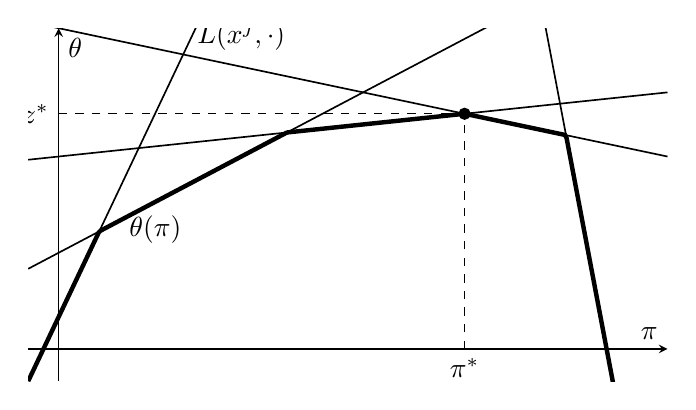
\begin{tikzpicture}
\begin{axis}[
    axis lines=middle,
    xlabel={$\pi$},
    ylabel={$\theta$},
    xmin=-1, xmax=20,
    ymin=-1, ymax=10,
    xtick=\empty,
    ytick=\empty,
    width=0.8\textwidth,
    height=0.5\textwidth,
    clip=true
]

% Define the five L(x^j, pi) lines
\addplot[domain=-1:20, samples=200, semithick] {2*x + 1};
\addplot[domain=-1:20, samples=200, semithick] {0.5*x + 3};
\addplot[domain=-1:20, samples=200, semithick] {0.1*x + 6};
\addplot[domain=-1:20, samples=200, semithick] {-0.2*x + 10};
\addplot[domain=-1:20, samples=200, semithick] {-5*x + 90};
\node[anchor=south] at (axis cs:6, 9) {$L(x^j,\cdot)$};

% Lower envelope (theta)
\addplot[domain=-1:20, samples=400, black, ultra thick] 
    {min(min(min(min(2*x+1,0.5*x+3),0.1*x+6),-0.2*x+10),-5*x+90)};
\node[anchor=south west, black, font=\bfseries] at (axis cs:2, 3) {$\mathbf{\theta(\pi)}$};
    
% Absolute maximum of the envelope
\addplot[only marks, mark=*, mark size=2pt] coordinates {(40/3, 22/3)};
\draw[dashed, thin] (axis cs:40/3,0) -- (axis cs:40/3,22/3);
\draw[dashed, thin] (axis cs:0,22/3) -- (axis cs:40/3,22/3);
\node[anchor=north] at (axis cs:40/3,0) {$\pi^*$};
\node[anchor=east]  at (axis cs:0,22/3) {$z^*$}; 

\end{axis}
\end{tikzpicture}
\caption{1D visualization of dual function $\theta(\pi)$ as envelope of Lagrangian functions $L(x^j, \cdot)$.}
\label{fig:cutting_plane}
\end{figure}

The dual problem~\eqref{eq:dual_problem} can be equivalently reformulated by introducing an auxiliary variable $\nu \in \mathbb{R}$ representing the value of the dual function. This yields
\begin{subequations} \label{eq:_dual_problem_cuts}
\begin{align}
z^* 
\; = \; \max_{\pi,\nu} \quad & \nu  \label{eq:_dual_problem_cuts_obj} \\
\text{s.t.} \quad 
& \nu \le b^\top \pi + (c - A^\top \pi)^\top x^j,
\quad \forall j \in \mathcal{J}, \label{eq:_dual_problem_cuts_constr} \\
& \pi \ge 0. \label{eq:_dual_problem_cuts_nonneg}
\end{align}
\end{subequations}
Each inequality in~\eqref{eq:_dual_problem_cuts_constr} corresponds to a so-called \textbf{dual cut}, providing a linear upper bound on $\nu$ for a specific column $x^j$.


\subsection{Row Generation in Dual Space}

We now repeat a similar derivation for the $k$-th iteration of the column generation algorithm, that is, for the $k$-th restricted master problem (RMP). Without loss of generality, we assume that the restricted index set is given by $\mathcal{J}^k  = \{1,\dots,k\} \subset \mathcal{J}.$

\begin{figure} [ht]
\centering

% -------- LEFT: full dual function theta --------
\begin{minipage}{0.48\textwidth}
\centering
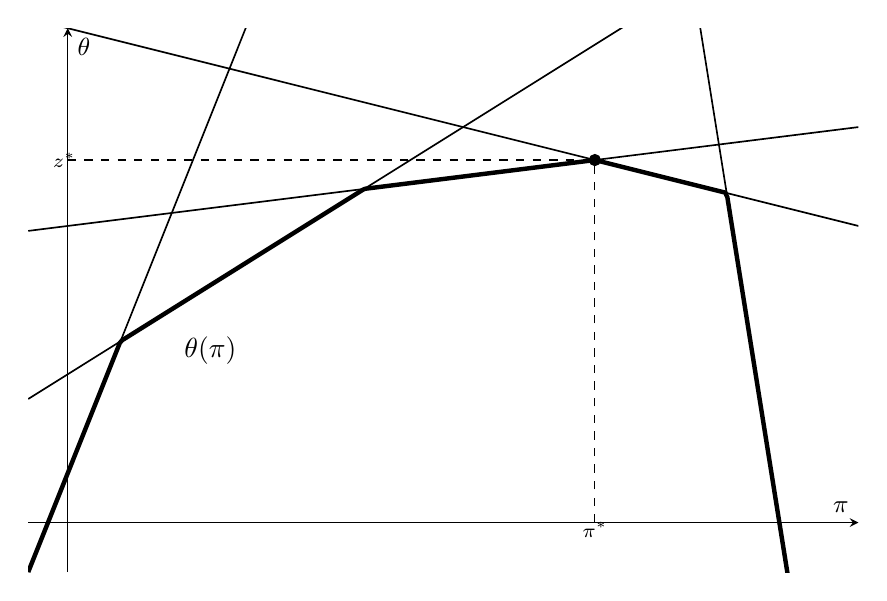
\begin{tikzpicture}
\begin{axis}[
    axis lines=middle,
    xlabel={$\pi$},
    ylabel={$\theta$},
    xmin=-1, xmax=20,
    ymin=-1, ymax=10,
    xtick=\empty,
    ytick=\empty,
    width=\textwidth,
    height=0.7\textwidth,
    clip=true,
    font=\small
]

% All five L(x^j, pi) lines
\addplot[domain=-1:20, samples=200, semithick] {2*x + 1};
\addplot[domain=-1:20, samples=200, semithick] {0.5*x + 3};
\addplot[domain=-1:20, samples=200, semithick] {0.1*x + 6};
\addplot[domain=-1:20, samples=200, semithick] {-0.2*x + 10};
\addplot[domain=-1:20, samples=200, semithick] {-5*x + 90};

% Full envelope theta
\addplot[domain=-1:20, samples=400, black, ultra thick] 
    {min(min(min(min(2*x+1,0.5*x+3),0.1*x+6),-0.2*x+10),-5*x+90)};
    
% Absolute maximum of the envelope
\addplot[only marks, mark=*, mark size=2pt] coordinates {(40/3, 22/3)};
\draw[dashed, thin] (axis cs:40/3,0) -- (axis cs:40/3,22/3);
\draw[dashed, thin] (axis cs:0,22/3) -- (axis cs:40/3,22/3);
\node[anchor=north, font=\scriptsize] at (axis cs:40/3,0.2) {$\pi^*$};
\node[anchor=east, font=\scriptsize]  at (axis cs:0.45,22/3) {$z^*$}; 

\node[anchor=south west, font=\bfseries] 
    at (axis cs:2.7,3) {$\mathbf{\theta(\pi)}$};

\end{axis}
\end{tikzpicture}
\end{minipage}
\hfill
% -------- RIGHT: restricted dual function theta^k --------
\begin{minipage}{0.48\textwidth}
\centering
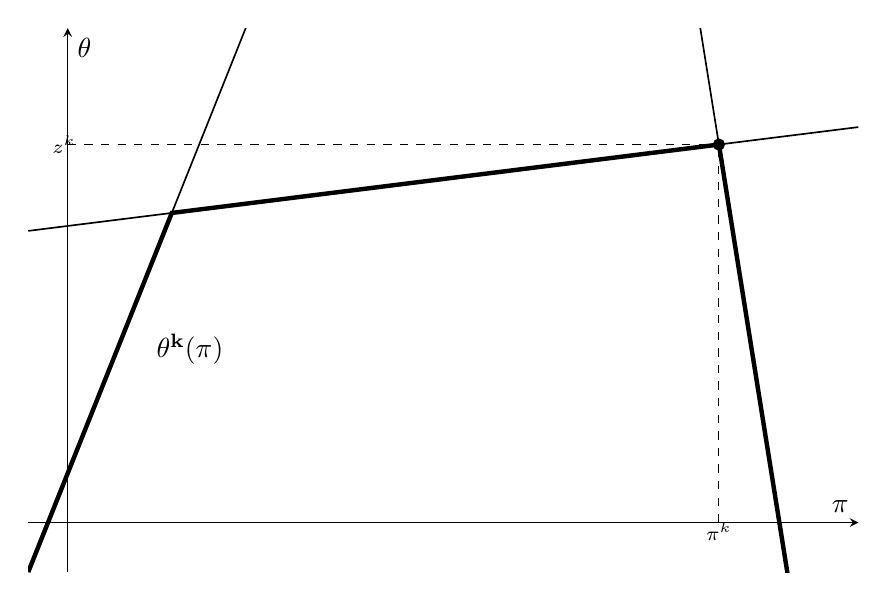
\begin{tikzpicture}
\begin{axis}[
    axis lines=middle,
    xlabel={$\pi$},
    ylabel={$\theta$},
    xmin=-1, xmax=20,
    ymin=-1, ymax=10,
    xtick=\empty,
    ytick=\empty,
    width=\textwidth,
    height=0.7\textwidth,
    clip=true
]

% Only first three L(x^j, pi) lines
\addplot[domain=-1:20, samples=200, semithick] {2*x + 1};
\addplot[domain=-1:20, samples=200, semithick] {0.1*x + 6};
\addplot[domain=-1:20, samples=200, semithick] {-5*x + 90};

% Restricted envelope theta^k for k=3
\addplot[domain=-1:20, samples=400, black, ultra thick] 
    {min(min(2*x+1,0.1*x + 6),-5*x + 90)};
    
% Absolute maximum of the envelope
\addplot[only marks, mark=*, mark size=2pt] coordinates {(16.47, 7.647)};
\draw[dashed, thin] (axis cs:16.47,0) -- (axis cs:16.47,7.647);
\draw[dashed, thin] (axis cs:0,7.647) -- (axis cs:16.47,7.647);
\node[anchor=north, font=\scriptsize] at (axis cs:16.47,0.2) {$\pi^k$};
\node[anchor=east, font=\scriptsize]  at (axis cs:0.45,7.647) {$z^k$}; 

\node[anchor=south west, font=\bfseries] 
    at (axis cs:2,3) {$\mathbf{\theta^k(\pi)}$};

\end{axis}
\end{tikzpicture}
\end{minipage}

\caption{Left: full dual function $\theta(\pi)$ as the lower envelope of all Lagrangian functions. Right: restricted dual function $\theta^k(\pi)$ for $k=3$.}
\label{fig:theta_vs_theta_k}
\end{figure}



The associated restricted dual function is then defined as
\[
\theta^k : \mathbb{R}_+^m \to \mathbb{R}, 
\quad
\pi \;\mapsto\; 
\theta^k(\pi) 
\;=\;
\min_{j=1,\dots,k} L(x^j,\pi)
\;=\;
\min_{j=1,\dots,k}
(c - A^\top \pi)^\top x^j + b^\top \pi.
\]
Since the minimum is taken over only a subset of all columns, the restricted dual function provides an upper approximation of the true dual function. In particular, for all $\pi \ge 0$,
\[
\theta^k(\pi) \;\ge\; \theta(\pi).
\]
In other words, the restricted model ignores some of the linear functions that define the true lower envelope, and therefore yields a value that is potentially too optimistic.

The dual problem corresponding to the restricted master problem is obtained by maximizing this restricted dual function,
\[
z^k
\;=\; \theta^k(\pi^k) \;=\;
\max_{\pi \ge 0}
\;
\theta^k(\pi),
\]
or equivalently using dual cuts,
\begin{subequations} \label{eq:restricted_dual_problem_cuts}
\begin{align}
z^k
\;=\;
\max_{\pi,\nu}
\quad & \nu
\label{eq:restricted_dual_problem_cuts_obj}
\\
\text{s.t.} \quad
& \nu 
\le
b^\top \pi 
+
(c - A^\top \pi)^\top x^j,
\qquad
j = 1,\dots,k,
\label{eq:restricted_dual_problem_cuts_constr}
\\
& \pi \ge 0.
\label{eq:restricted_dual_problem_cuts_nonneg}
\end{align}
\end{subequations}
This formulation naturally suggests an iterative solution procedure. At iteration $k$, we first solve the restricted dual problem~\eqref{eq:restricted_dual_problem_cuts} to obtain an optimal dual solution $\pi^k$. Using this solution, we then solve the pricing problem to identify a new column
\[
x^{k+1} \; = \; x(\pi^k) \; \in \;
\arg\min_{x \in X}
\;
(c - A^\top \pi^k)^\top x.
\]
We then compare the value of the newly identified column with the current restricted dual value:
\[
\theta(\pi^k) = L(x^{k+1}, \pi^k) \quad \text{versus} \quad \theta^k(\pi^k) = \min_{j=1,\dots,k} L(x^j, \pi^k).
\]

\begin{itemize}
    \item If $\theta(\pi^k) < \theta^k(\pi^k)$, the new column $x^{k+1}$ defines a violated dual inequality. We add $x^{k+1}$ to the restricted set and continue the iteration.
    \item If $\theta(\pi^k) \geq \theta^k(\pi^k)$, no column improves the restricted dual. The current solution $\pi^k$ maximizes the full dual function $\theta(\pi)$, and the algorithm terminates.
\end{itemize}

This condition corresponds exactly to the stopping criterion of the column generation algorithm. To make this explicit, observe first that
\[
L(x^j,\pi^k)
= c^T x^j - (\pi^k)^T A x^j + (\pi^k)^T b
= \bar{c}_j(\pi^k) + (\pi^k)^T b,
\]
where $\bar{c}_j(\pi^k)$ denotes the reduced cost of column $x^j$ at dual point $\pi^k$.
Since the term $(\pi^k)^T b$ is independent of $j$, it cancels in the comparison of different columns, and we obtain
\[
\theta(\pi^k) - \theta^k(\pi^k)
=
\min_{j \in \mathcal{J}} L(x^j,\pi^k)
-
\min_{j \in \mathcal{J}^k} L(x^j,\pi^k)
=
\min_{j \in \mathcal{J}} \bar{c}_j(\pi^k)
-
\min_{j \in \mathcal{J}^k} \bar{c}_j(\pi^k).
\]
At an optimal solution of the restricted master problem, all columns in $\mathcal{J}^k$ have non-negative reduced cost, so that
\[
\theta(\pi^k) - \theta^k(\pi^k)
=
\min_{j \in \mathcal{J}} \bar{c}_j(\pi^k)
=
\min_{j \in \mathcal{J} \setminus \mathcal{J}^k} \bar{c}_j(\pi^k).
\]
This shows that the gap is exactly determined by the most negative reduced cost among all columns not yet included in the restricted master problem. In particular, the stopping criteria are equivalent:
\[
\theta(\pi^k) \geq \theta^k(\pi^k) \qquad \Longleftrightarrow \qquad \min_{j \in \mathcal{J} \setminus \mathcal{J}^k} \bar{c}_j(\pi^k) \ge 0.
\]
There is a natural geometric interpretation underlying this procedure. The primal master problem can be viewed as involving a full (potentially very large) set of columns, although only a small subset is active at optimality and contributes to the optimal solution. In dual space, the corresponding formulation involves a full collection of affine dual cuts, of which again only a small subset is active and determines the optimal value. Column generation can then be understood as iteratively discovering these relevant primal columns, one per iteration, until the correct subset that supports the optimal solution has been identified. Equivalently, in dual space, this corresponds to progressively revealing the active dual cuts, until the finite set of supporting hyperplanes that define the optimal dual solution has been recovered. Because of this equivalence, in the dual space the algorithm is often referred to as \textbf{row generation}.


\subsection{Row Generation for Constraint Shortest Path Problems}

We now revisit the constrained shortest path problem (CSPP) introduced in Chapter~\ref{chap:column_generation}, using it to illustrate the column generation process in dual space. Recall that the network, shown in Figure~\ref{fig:tcsp-network}, consists of nodes connected by directed edges, where each edge $(i,j)$ has a cost $c_{ij}$ and a traversal time $t_{ij}$. The goal is to find a path from the source node $1$ to the sink node $6$ that minimizes the total cost while ensuring the total traversal time does not exceed $T = 14$ units.
\begin{figure}[ht]
    \centering
    \includegraphics[width=0.7\textwidth]{dual_space_all.png}
    \caption{Dual function $\theta(\pi)$ defined as lower envelope of the 9 Lagrangian functions.}
    \label{fig:lagrangian_dual}
\end{figure}

In total, one can count 9 different feasible paths from the source to the sink. This means that we have 9 extreme points $x^j \in \{0,1\}^{10}$ and hence we can define the corresponding Lagrangian functions as in (\ref{eq:Lagrangian}):
\[
L(x^j, \pi) = c^\top x^j - \pi \, (14 - t^\top x^j), \qquad j = 1, \dots, 9, \; \; \pi \geq 0,
\]
where $c \in \mathbb{R}^{10}$ is the edge cost and $t \in \mathbb{R}^{10}$ is the edge traversal time.
The dual function is then the lower envelope of all the above Lagrangian functions, which has been illustrated in Figure~\ref{fig:lagrangian_dual}. From this figure, we can see that the optimal value is at $(\pi^*, \nu^*) = (2,7)$, meaning $\pi^* = 2$ is the optimal Lagrange multiplier for the time constraint with optimal cost $7$.


\begin{table}[ht]
\centering
\footnotesize
\renewcommand{\arraystretch}{1.3}
\begin{tabular}{c|c|c|c|c|c}
\hline
Iteration 
& Active paths 
& $\lambda$ values 
& $(\pi_{\text{time}}, \pi_{\text{convex}})$ 
& $z_{RMP}^*$ 
& Min. reduced cost \\ 
\hline

1 
& $\{1246, 1356\}$ 
& $(0.6,\;0.4)$ 
& $(2.1,\;40.8)$ 
& 11.4 
& $13256:\ \bar{c}=-4.8$ \\

\hline

2 
& $\{1246, 1356, 13256\}$ 
& $(0.5,\;0,\;0.5)$ 
& $(1.5,\;30.0)$ 
& 9.0 
& $1256:\ \bar{c}=-2.5$ \\

\hline

3 
& $\{1246, 1356, 13256, 1256\}$ 
& $(0,\;0,\;0.2,\;0.8)$ 
& $(2.0,\;35.0)$ 
& 7.0 
& none ($\bar{c}_p \ge 0$) \\

\hline
\end{tabular}
\caption{Column generation steps for the CSPP illustrated in Figure~\ref{fig:tcsp-network}.}
\label{tab:cg_steps_cpp}
\end{table}

Starting from a restricted path set containing the paths $1246$ and $1356$, column generation produces the sequence of iterations shown in Table~\ref{tab:cg_steps_cpp}, as discussed in Subsection~\ref{subsec:cg_example}. Each iteration consists of solving the restricted master problem, computing the associated dual solution, and using it in the pricing problem to generate an improving path.

\bigskip

It is now natural to reinterpret the algorithm from a dual perspective. As shown earlier, column generation can be viewed as a cutting-planes method in the space of Lagrangian functions, where each newly generated path $x^j$ introduces an additional linear function $L(x^j,\pi)$ that refines the lower envelope of the dual function. Figures~\ref{fig:dual_space_iter1}, \ref{fig:dual_space_iter2}, and \ref{fig:dual_space_iter3} illustrate the evolution of the dual space at each iteration of the algorithm. In each figure, the current collection of Lagrangian functions defining the restricted dual model is shown together with the full dual function $\theta(\pi)$ for reference.
\begin{figure}[ht]
    \centering
    \includegraphics[width=0.7\textwidth]{dual_space_iter1.png}
    \caption{Iteration 1: dual function based on initial paths $1246$ and $1356$.}
    \label{fig:dual_space_iter1}
\end{figure}

We start with only the two initial paths $1246$ and $1356$, corresponding to the two Lagrangian functions shown in Figure~\ref{fig:dual_space_iter1}. The resulting restricted dual function is denoted by $\theta^{1}(\pi)$, defined as the lower envelope of these two lines. Maximizing this function gives the familiar RMP solution
\[
\pi^{1} = 2.1, \qquad \theta^{1}(\pi^{1}) = 11.4.
\]

If we evaluate this dual point in the full dual function $\theta(\pi)$, we obtain $\theta(\pi^{1}) = 6.6$, which represents the lower bound of the RMP objective. This also implies that the gap $\theta(\pi^{1}) - \theta^{1}(\pi^{1})$
corresponds exactly to the most negative reduced cost $-4.8$. Geometrically, the point $(\pi^{1}, \theta(\pi^{1}))$ lies on a new Lagrangian line, which identifies path $13256$ as the entering column.
\begin{figure}[ht]
    \centering
    \includegraphics[width=0.7\textwidth]{dual_space_iter2.png}
    \caption{Iteration 2: dual function after adding path $13256$.}
    \label{fig:dual_space_iter2}
\end{figure}

After adding path $13256$, the restricted dual function is updated to include three Lagrangian lines. However, notice that the lower envelope $\theta^2(\pi)$ does not use path $1356$ for its optimal point $\pi^2$, which is consistent with Table~\ref{tab:cg_steps_cpp}. The maximization of the new envelope yields
$\pi^{2} = 1.5$ and $\theta^{2}(\pi^{2}) = 9.0$.
At this point, the pricing problem identifies path $1256$ as the most violated constraint, corresponding to the next Lagrangian line entering the envelope.
\begin{figure}[ht]
    \centering
    \includegraphics[width=0.75\textwidth]{dual_space_iter3.png}
    \caption{Iteration 3: final dual function where no violated constraints remain.}
    \label{fig:dual_space_iter3}
\end{figure}

After adding path $1256$, the maximizer of the restricted dual function becomes $\pi^{3} = 2.0$ with optimal value $\theta^{3}(\pi^{3}) = 7.0$.
At this point, this solution already lies on the true dual function, i.e., $\theta^{3}(\pi^{3}) = \theta(\pi^{3})$. Hence the gap between the restricted and full dual function is zero, which implies that the reduced cost of all paths is non-negative. Consequently, no further violated constraints exist, and the algorithm terminates with the optimal solution.


\newpage


\subsection{Instability and Convergence Issues in Dual Space}

The row-generation interpretation developed in the previous subsections admits a well-known equivalent formulation in the literature and can be understood as an application of \textbf{Kelley's cutting plane method} \cite{Kelley1960} to the maximization of a \textbf{nonsmooth, concave, piecewise-linear function}. This connection was first made explicit in \cite{duMerle1999} and has since become a standard viewpoint in the column generation literature (see, e.g., \cite{briant2008, Lubbecke2011}). It also helps explain the gap between the strong theoretical guarantees of column generation and its often weaker behaviour in practice. Through this equivalence, the method can be interpreted from the perspective of nonsmooth optimization, where Kelley's cutting plane method is well studied and known to perform poorly in practice, in particular due to \textbf{instability} and \textbf{slow convergence}.

\bigskip

Kelley's cutting plane method builds a piecewise-linear approximation of the objective function using first-order (subgradient) information. Each subgradient defines a supporting hyperplane that is most accurate near the point where it was generated. By taking the maximum over all such hyperplanes, the algorithm obtains a global approximation of the function. However, while each approximation is locally meaningful, the method always optimizes this model over the entire space, without any restriction that keeps successive iterates close to one another. As a result, the solution of the model can shift to regions where completely different hyperplanes dominate, leading to \textbf{large jumps between iterates}. This explains the typical \textbf{zigzag behaviour}, where the method moves back and forth between different regions because the local approximations keep changing, rather than following a smooth path toward the optimum.

\bigskip

This zigzagging is problematic because it prevents the algorithm from exploiting good intermediate solutions. Even if an iterate is already close to the optimal solution $\pi^*$, the next iterate may move far away again, simply because the global model suggests a different extreme point. In other words, the method has no mechanism to stay near or refine a good solution once it has been found. As a consequence, progress made in one iteration can be lost in the next, leading to \textbf{instability in the iterates} and \textbf{inefficient use of information}. This behaviour is a key reason for the slow convergence of Kelley's method, and, due to the equivalence discussed earlier, directly explains the instability and poor practical performance observed in column generation \cite{benamor2009stabilizing}.

\bigskip

Another important aspect of our setting is that the dual function $\theta(\pi)$ is itself piecewise linear. As a result, the optimal solution is determined by the intersection of a finite number of supporting hyperplanes. In principle, this means that Kelley's method can reach the exact optimum in finitely many steps, since it gradually reconstructs these hyperplanes \cite{ruszczynski2006nonlinear}.

However, this also explains the \textbf{slow convergence near optimality}. During the iterations, the algorithm only recovers parts of the true function. While the approximation may already be very accurate close to the optimum, the exact solution can only be identified once all hyperplanes that define the optimal point have been found.

Near the end, this becomes difficult because the remaining missing hyperplanes are precisely those that are active at optimality, and they must be discovered one by one. Until this exact set is identified, the algorithm cannot fully lock onto the optimal point, even if it is already very close. As a result, progress becomes very small and slow, leading to the well-known \textbf{tailing-off effect}.

\bigskip

Another important practical issue arises already at the initialization of the algorithm. To obtain a feasible starting point, artificial columns with large penalty costs are typically introduced. While this ensures that the initial restricted master problem is well-defined, it also induces dual solutions that are far from the true optimal dual solution. Since the quality of the generated columns strongly depends on the dual variables, poor initial dual estimates lead to the generation of \textbf{low-quality columns} in the early iterations. In dual space, this means that the algorithm starts in a region that is not representative of the true structure of the problem, and therefore constructs cuts that are largely irrelevant for the optimal solution. As a result, the method may spend many iterations correcting this poor starting point before meaningful progress is made, which further contributes to the \textbf{slow practical performance of column generation}.


\section{Stabilization in Column Generation}

Building on the equivalence discussed above, it may at first seem surprising that classical column generation is used so widely in large-scale linear optimization problems. After all, we have just seen that it is algorithmically equivalent to Kelley's cutting plane method applied to a nonsmooth, piecewise-linear concave function, and this method is well known in nonsmooth optimization to behave poorly in its basic form. It often produces unstable iterates and slow progress. This naturally raises the question why it still works in practice. The main reason is that a large part of the literature has been devoted precisely to fixing these weaknesses through stabilization techniques.

\bigskip

The central idea behind stabilization is simple. Kelley's method can produce iterates that jump far away from a good solution because it always optimizes a global piecewise-linear model without any notion of locality. Stabilization methods aim to prevent this behaviour by encouraging the algorithm to stay \textit{near} promising dual solutions or by discouraging overly large steps.

One of the earliest and most intuitive ideas is the \textbf{boxstep method} \cite{marsten1975boxstep}. This approach restricts each iterate to lie inside a box around the current reference point. In other words, instead of allowing the dual solution to move freely to any optimizer of the global model, the update is constrained component-wise to remain within a fixed neighbourhood. This often improves numerical stability and leads to more controlled progress in practice. However, the method is sensitive to the choice of the box size, since the restriction is purely coordinate-wise and does not adapt to the underlying geometry of the problem. As a result, inappropriate scaling or parameter choices can still lead to slow convergence or overly conservative steps.

\bigskip

A related but more flexible idea was later developed in the context of column generation by du Merle et al. \cite{duMerle1999}. Their approach, often referred to as the \textbf{BoxPen method}, remains within the linear programming framework but replaces the hard box restriction by a softer form of stabilization. Instead of strictly constraining the dual variables to lie within a fixed box, deviations from a reference point are penalized or modeled through additional linear variables and constraints. This reduces the tendency of Kelley-type iterations to produce extreme jumps while preserving an LP structure. However, the resulting formulation is more involved, and its performance depends on the choice of stabilization parameters that control the strength of the penalty, which may require careful tuning in practice.

\bigskip

Another approach moves away from the LP structure altogether. In \textbf{bundle methods} (see, e.g., \cite{hiriarturruty1993convex, lemarechal1995new, kiwiel1990proximity}), stabilization is achieved by adding a quadratic proximal term to the model. Instead of maximizing a piecewise-linear approximation, the method penalizes movements away from the current reference point in a smooth quadratic way. This creates a kind of \textit{tethering} effect, meaning the algorithm is encouraged to improve the solution, but large steps are gradually penalized. In a column generation context, this comes at the cost that each iteration typically requires solving a quadratic program instead of a linear program, which is generally more computationally demanding.

\bigskip

For a more detailed and comprehensive overview of stabilization techniques in column generation, including computational comparisons and practical implementations, we refer the reader to \cite{briant2008, benamor2009stabilizing}.

\bigskip

Finally, a fundamentally different approach avoids extreme-point solutions altogether by relying on \textbf{interior point methods}. Instead of solving the restricted master problem with the simplex method, which produces vertex solutions and thus contributes to the zigzag behaviour, interior point methods follow a path through the interior of the feasible region. This leads to much smoother sequences of dual variables and can significantly reduce instability. In the context of column generation, Rousseau et al.~\cite{rousseau2007interior} propose such an interior point stabilization approach, showing that it can improve convergence behaviour in practice. However, these methods also come with drawbacks, most notably that they are more difficult to warm-start between iterations, which limits their efficiency in a column generation framework where problems are solved repeatedly with small changes.


\subsection{Bundle Method in Dual Space}

In this work, we study the bundle method in more detail as a stabilization approach. As discussed in the previous section, several techniques exist to stabilize Kelley-type methods. Among these, the bundle method is particularly attractive because it stabilizes the iterates through a smooth proximal term, instead of restricting them with hard bounds. The main disadvantage is that the problem is no longer linear. Each iteration requires solving a quadratic program instead of a linear program. However, as we will show in Chapter~\ref{chap:regularized column generation}, this additional structure can be efficiently handled in a column generation setting using a hot-started active-set method, so the computational cost remains manageable in practice.

We now describe the bundle method in more detail from a theoretical point of view \cite{briant2008, ruszczynski2006nonlinear}.

\bigskip

As we have observed, the maximization of the restricted model $\theta^k(\pi)$ is often overly optimistic, in the sense that it encourages iterates to move toward regions where the approximation is still unreliable. This motivates a more cautious strategy in which the next iterate is not chosen solely based on optimality with respect to $\theta^k$, but is also influenced by its proximity to previously identified reliable solutions.
In particular, it is penalized for being too far away from a region of good previous iterates. In this way, the algorithm is prevented from making arbitrarily large jumps unless such moves are strongly justified by a significant improvement in the model value.

\bigskip

We begin by identifying a set of bounds that are available at every iteration $k$ of the column generation algorithm. In particular, for the current restricted solution $\pi^k$, we always have the relation
\[
\theta(\pi^k) \;\le\; \theta(\pi^\star) \;\le\; \theta^k(\pi^k),
\]
where $\theta(\pi^k)$ is the value of the true dual function at the current iterate, $\theta(\pi^\star)$ is the optimal dual value, and $\theta^k(\pi^k)$ is the optimal value of the restricted dual problem.

However, the sequence $\theta(\pi^k)$ is generally not monotone. A stronger and more informative lower bound is obtained by keeping track of the best dual iterate encountered so far. We therefore define the \textbf{stability center}
\[
\hat{\pi}^k
\;=\;
\arg\max_{i=1,\dots,k} \; \theta(\pi^i),
\]
that is, the iterate that yields the largest true dual value among all iterates up to iteration $k$. Consequently, we obtain the refined chain of bounds
\[
\theta(\pi^k)
\;\le\;
\theta(\hat{\pi}^k)
\;\le\;
\theta(\pi^\star)
\;\le\;
\theta^k(\pi^k).
\]
This sequence of bounds naturally motivates the definition of a region in the $(\pi,\theta)$-space determined by the lower bound $\theta(\hat{\pi}^k)$ together with the current collection of Lagrangian cuts and the upper bound $\theta^k(\pi^k)$. In Figure~\ref{fig:dual_space_region}, we zoom in on our example at iteration $k=2$ around the region of interest. In this case, $\hat{\pi}^2 = 2.1$ with lower bound value $\theta(\hat{\pi}^2) = 6.6$. From the inequalities above, it follows that the optimal solution $(\pi^\star,\theta(\pi^\star))$ must lie inside this region.

\begin{figure}[ht]
    \centering
    \includegraphics[width=0.75\textwidth]{dual_space_region.png}
    \caption{Safeguard region for the dual problem at iteration $k=2$.}
    \label{fig:dual_space_region}
\end{figure}

\bigskip

The classical cutting-planes (or column generation) algorithm selects the point that maximizes the current model, that is, the highest point of this region. As discussed in the previous subsection, this choice is often overly optimistic in practice. The model $\theta^k$ may significantly overestimate the true function $\theta$, leading to large oscillations of the iterates and slow convergence.
A more robust strategy is therefore to select a new iterate that remains closer to the stability center $\hat{\pi}^k$, rather than always moving to the maximizer of the current model.

\bigskip

This idea can be implemented by replacing the pure maximization of the restricted model $\theta^k(\pi)$ with a stabilized objective that penalizes deviations from the stability center. More precisely, we consider the modified problem
\[
\max_{\pi \ge 0} \;\; \theta^k(\pi) - S(\pi - \hat{\pi}^k),
\]
where $S(\cdot)$ is a stabilization function satisfying $\min_{\pi \ge 0} S(\pi) = 0$ and increasing with the distance from $\hat{\pi}^k$. This term acts as a regularization that pulls the iterates towards the current best point $\hat{\pi}^k$, thereby reducing oscillations in the dual sequence.

\bigskip

Different choices of stabilization functions are possible and are discussed in \cite{briant2008}. In this work, we focus on a quadratic proximal term, leading to the stabilized dual master problem
\begin{equation} \label{eq:bundle_method}
\max_{\pi \ge 0} \;\; \theta^k(\pi) - \frac{\delta}{2}\|\pi - \hat{\pi}^k\|^2,
\end{equation}
where $\delta > 0$ controls the strength of the regularization. In contrast to the original cutting-planes formulation, the stabilized dual master problem \eqref{eq:bundle_method} is no longer a piecewise-linear program, but instead a quadratic optimization problem. This introduces an additional computational cost per iteration, since quadratic programs are typically more expensive to solve than linear programs. However, this is compensated by a significant improvement in stability and convergence behaviour.

\bigskip

An additional advantage of this formulation is that it naturally resolves the initialization issue encountered in the pure cutting-planes approach. In particular, the method can be started without any initial set of columns by choosing an initial stability center, often based on a heuristic or simply $\hat{\pi}^0 = 0$, and setting the first iterate equal to this point.


\subsection{Bundle Method for the Constraint Shortest Path Example}

We now apply the stabilization idea to the constrained shortest path example introduced earlier. In the previous section, the column generation algorithm was initialized with two existing paths, namely $\mathcal{P} = \{1246, 1356\}$. These two paths were not chosen arbitrarily, but were obtained from a classical Big-$M$ initialization procedure in which artificial variables were temporarily introduced to ensure feasibility of the initial restricted master problem. After two initialization iterations, these artificial variables left the two feasible paths as the starting set.

\bigskip

As discussed in the previous subsection, stabilization allows us to initialize the algorithm in a simpler way. In particular, the method can be started with only a single path. For the present example, we therefore initialize the restricted path set with the single path $1246$. Furthermore, we fix the stabilization parameter to $\delta = 1.0$ and choose the initial stability center $\hat{\pi}^{1} = 0.0$.
Because a single Lagrangian function combined with the quadratic penalty defines a concave quadratic function, the stabilized restricted model always admits a unique maximizer. 

\begin{figure}[ht]
    \centering
    \includegraphics[width=0.75\textwidth]{dual_stab_iter1.png}
    \caption{Iteration 1 of the stabilized method starting from a single path $1246$.}
    \label{fig:dual_stab_iter1}
\end{figure}

Figure~\ref{fig:dual_stab_iter1} illustrates the first iteration of the stabilized method. In this case, the maximizer of the stabilized restricted function is $\pi^{1} = 4.0$ with $\theta(\pi^{1}) = -1.0$. Since the obtained value satisfies $\theta(\pi^{1}) < \theta(\hat{\pi}^{1})$,
the new iterate does not improve the current best dual value. Consequently, the stability center is not updated and remains $\hat{\pi}^{2} = 0.0$.
Projecting the point $\pi^{1}$ onto the true dual function $\theta(\pi)$ identifies the Lagrangian function corresponding to path $13256$, which is therefore added to the restricted model.

\bigskip

\begin{figure}[ht]
    \centering
    \includegraphics[width=0.73\textwidth]{dual_stab_iter2.png}
    \caption{Iteration 2 of the stabilized method after adding path $13256$.}
    \label{fig:dual_stab_iter2}
\end{figure}

The next iteration is shown in Figure~\ref{fig:dual_stab_iter2}. After adding the new path, the stabilized restricted problem yields the solution
$\pi^{2} = 1.5$ with $\theta(\pi^{2}) = 6.5$.
In this figure, one can clearly observe that the algorithm does not move to the maximal value of the current piecewise-linear model, that is, the highest point in the safeguard region. Instead, it selects a more central and less optimistic point that remains closer to the stability center. Because the new iterate improves the true dual value, the stability center is updated according to $\hat{\pi}^{3} = 1.5$.
Once again, the projection onto the full dual function indicates that path $1256$ has negative reduced cost, and this path is therefore added to the restricted model.

\bigskip

The subsequent iteration is illustrated in Figure~\ref{fig:dual_stab_iter3}. Solving the stabilized restricted problem now results in $\pi^{3} = 2.0$ and $\theta(\pi^{3}) = 6.88$. At this point, the effect of stabilization becomes particularly visible. The quadratic penalty acts as a smooth approximation of the current piecewise-linear model. In other words, the method attempts to approximate the dual function locally using a quadratic model rather than relying on the piecewise-linear envelope. In this iteration, the minimal reduced cost can be computed in the same way as before and is found to be zero. Hence no further violated constraints exist, and the algorithm terminates.

\begin{figure}[ht!]
    \centering
    \includegraphics[width=0.73\textwidth]{dual_stab_iter3.png}
    \caption{Iteration 3 of the stabilized method.}
    \label{fig:dual_stab_iter3}
\end{figure}


It is worth noting that this solution represents an approximation of the exact dual optimum obtained without stabilization. In this small example, the difference is negligible, but in larger problems the stabilized method typically produces a sequence of iterates that converges more reliably and with significantly reduced oscillations. For a detailed computational study demonstrating these effects, we refer to Section~\ref{chap:Implementation and Computational Results}, where the stabilized algorithm is tested extensively on more realistic problem instances.



\subsection{Stabilization in Primal Space}

Although the dual interpretation of stabilization provides valuable insight into the behaviour of column generation, the ultimate goal remains the computation of an optimal primal solution. We therefore now reformulate the stabilized dual problem in the primal space. Starting from the stabilized dual formulation
\begin{align}
\max_{\nu,\pi} \quad 
    & \nu - \frac{\delta}{2}\|\pi - \hat{\pi}\|^2 
    \label{eq:stabilized_dual} \\
\text{s.t.} \quad 
    & \nu \le b^\top \pi + (c - A^\top \pi)^\top x^j,
    \quad \forall j \in \mathcal{J}, \nonumber \\
    & \pi \ge 0, \nonumber
\end{align}
we now express the same problem in terms of primal variables only. The resulting formulation can be interpreted as a stabilized version of the master problem, where the original linear programming structure is augmented with a quadratic regularization term that penalizes deviations of the dual variables from the stability center. 

\medskip

\paragraph{Lagrangian formulation.}

To derive the corresponding primal formulation, we begin by writing the Lagrangian function associated with the constraints in~\eqref{eq:stabilized_dual}. Let $\lambda_j \ge 0$ denote the Lagrange multiplier corresponding to the $j$-th inequality constraint. The Lagrangian is then given by
\begin{align}
\mathcal{L}(\pi,\nu,\lambda)
=
\nu
- \frac{\delta}{2}\|\pi - \hat{\pi}\|^2
+
\sum_{j \in \mathcal{J}}
\lambda_j
\Big(
b^\top \pi
+
(c - A^\top \pi)^\top x^j
-
\nu
\Big).
\end{align}

We now rearrange the terms by collecting the coefficients of $\nu$,
\begin{align}
\mathcal{L}(\pi,\nu,\lambda)
=
\nu
\Big(
1 - \sum_{j \in \mathcal{J}} \lambda_j
\Big)
-
\frac{\delta}{2}\|\pi - \hat{\pi}\|^2
+
\sum_{j \in \mathcal{J}}
\lambda_j
\Big(
b^\top \pi
+
(c - A^\top \pi)^\top x^j
\Big),
\end{align}

and expand the remaining terms:
\begin{align}
\mathcal{L}(\pi,\nu,\lambda)
=
\nu
\Big(
1 - \sum_{j} \lambda_j
\Big)
-
\frac{\delta}{2}\|\pi - \hat{\pi}\|^2
+
\sum_{j}
\lambda_j c^\top x^j
-
\sum_{j}
\lambda_j \pi^\top A x^j
+
\sum_{j}
\lambda_j b^\top \pi .
\end{align}
To obtain a compact representation, we stack all feasible columns $x^j$ into a matrix
\[
X =
\begin{bmatrix}
x^1 & x^2 & \cdots & x^{|J|}
\end{bmatrix}.
\]

Furthermore, let $\lambda \in \mathbb{R}^{|J|}$ denote the vector of multipliers and let $\mathbf{1}$ denote a vector of ones. Using matrix notation, the Lagrangian can be written as
\begin{align}
\mathcal{L}(\pi,\nu,\lambda)
=
\nu
\big(
1 - \mathbf{1}^\top \lambda
\big)
-
\frac{\delta}{2}\|\pi - \hat{\pi}\|^2
+
c^\top X \lambda
-
\pi^\top A X \lambda
+
b^\top \pi \,
\mathbf{1}^\top \lambda .
\end{align}

Grouping the terms involving $\pi$ yields
\begin{align}
\mathcal{L}(\pi,\nu,\lambda)
=
\nu
\big(
1 - \mathbf{1}^\top \lambda
\big)
-
\frac{\delta}{2}\|\pi - \hat{\pi}\|^2
+
c^\top X \lambda
+
\pi^\top
\big(
b \mathbf{1}^\top
-
A X
\big) \lambda.
\end{align}

\medskip

\paragraph{Dual function.}

We now derive the dual function
\[
g(\lambda)
=
\inf_{\pi,\nu}
\mathcal{L}(\pi,\nu,\lambda).
\]

We first minimize with respect to $\nu$. Since the Lagrangian is linear in $\nu$, the infimum is finite only if
$\mathbf{1}^\top \lambda = 1,$
which yields the familiar convexity constraint from column generation. Under this condition and using an auxiliary variable
\begin{align} \label{eq:w-substitution}
w
=
\frac{1}{\delta}
\big(
b - A X \lambda
\big),
\end{align}
the Lagrangian simplifies to
\begin{align}
\mathcal{L}(\pi,\lambda)
=
-
\frac{\delta}{2}\|\pi - \hat{\pi}\|^2
+
\delta w^\top \pi
+
c^\top X \lambda.
\end{align}
Next, we minimize with respect to $\pi$ which is obtained by setting the gradient equal to zero:
\begin{align} \label{eq:expression_pi}
\pi
=
\hat{\pi}
+
w.
\end{align}
Substituting this expression back into the Lagrangian yields the dual function
\begin{align}
g(\lambda) 
= c^\top X \lambda + \delta \hat{\pi}^\top w - \frac{\delta}{2} \| w \|^2 
= c^\top X \lambda + \frac{\delta}{2} \| w + \hat{\pi} \|^2 - \frac{\delta}{2} \| \hat{\pi} \|^2 .
\end{align}
Therefore, the stabilized problem expressed in the primal space becomes
\begin{subequations}
\label{eq:stabilized_primal}
\begin{align}
\min_{\lambda, w}
\quad
&
c^\top X \lambda
+
\frac{\delta}{2} \| w + \hat{\pi} \|^2
-
\frac{\delta}{2} \| \hat{\pi} \|^2
\label{eq:stabilized_primal_obj}
\\
\text{s.t.}
\quad
&
A X \lambda + \delta w = b,
\label{eq:stabilized_primal_link}
\\
&
\mathbf{1}^\top \lambda = 1,
\label{eq:stabilized_primal_convexity}
\\
&
\lambda \ge 0.
\label{eq:stabilized_primal_nonneg}
\end{align}
\end{subequations}

This formulation has a very familiar structure when compared to the classical Dantzig--Wolfe master problem. In particular, the variables $\lambda$ still represent a convex combination of columns, enforced by the convexity constraint~\eqref{eq:stabilized_primal_convexity}. As in the standard master problem, this constraint is associated with a Lagrange multiplier, which we denote by $\pi_0$. The objective function in~\eqref{eq:stabilized_primal_obj}, however, differs from the linear objective of the classical formulation. Due to the stabilization term introduced in the dual space, the objective is now a convex quadratic function. Constraint~\eqref{eq:stabilized_primal_link} can be interpreted as a slightly modified version of the usual linking constraint in the Dantzig--Wolfe master problem. In the classical setting, this constraint would simply read $A X \lambda = b$.
Here, the additional term $\delta w$ reflects the effect of stabilization. Despite this modification, the constraint still gives the familiar dual variable 
$\pi$, which can be recovered from the relation \eqref{eq:expression_pi}. 

\bigskip

Finally, observe that the constant term 
\[
- \frac{\delta}{2} \|\hat{\pi}\|^2
\]
in the objective~\eqref{eq:stabilized_primal_obj} does not depend on the decision variables $\lambda$ or $w$. Therefore, it can be omitted when determining the optimal solution of problem~\eqref{eq:stabilized_primal}, although it must be taken into account when evaluating the optimal objective value.


\paragraph{Eliminating auxiliary variable $\mathbf{w}$.}
Note that the linking constraint~\eqref{eq:stabilized_primal_link} is just a simple substitution, which implies that the auxiliary variable $w$ can be eliminated from the formulation. Indeed, substituting~\eqref{eq:w-substitution} into the quadratic term of the objective function gives
\begin{align}
\frac{\delta}{2}
\|
w + \hat{\pi}
\|^2
=
\frac{\delta}{2}
\left\|
\frac{1}{\delta}
(
b - A X \lambda
)
+
\hat{\pi}
\right\|^2
=
\frac{1}{2 \delta}
\left\|
(\delta \hat{\pi}
+
b) - A X \lambda
\right\|^2.
\end{align}
We can further expand the squared norm by grouping the constant terms together:
\begin{align}
\frac{1}{2 \delta}
\left\|
(\delta \hat{\pi}
+
b) - A X \lambda
\right\|^2
&=
\frac{1}{2 \delta}
\Big(
\|
\delta \hat{\pi} + b
\|^2
-
2
(\delta \hat{\pi} + b)^\top
A X \lambda
+
\|
A X \lambda
\|^2
\Big)
\\
&= 
\frac{1}{2 \delta}
\|
\delta \hat{\pi} + b
\|^2
-
\frac{1}{\delta}
(\delta \hat{\pi} + b)^\top
A X \lambda
+
\frac{1}{2 \delta}
\|
A X \lambda
\|^2. \label{eq:expanded_norm}
\end{align}
The first term of \eqref{eq:expanded_norm} is independent of $\lambda$, hence we omit it when determining the optimal solution.
Then, the full expanded objective for \eqref{eq:stabilized_primal} is given by
\begin{align}
c^\top X \lambda
- \bigl( \frac{b}{\delta} + \hat{\pi} \bigr)^\top A X \lambda
+ \frac{1}{2\delta} \| A X \lambda \|^2
&=
\Bigl( c^\top X - \bigl( \frac{b}{\delta} + \hat{\pi} \bigr)^\top A X \Bigr) \lambda
+ \frac{1}{2\delta} \| A X \lambda \|^2.
\end{align}
Consequently, the stabilized master problem can be written entirely in terms of the variables $\lambda$ as
\begin{subequations} \label{eq:stab-elminated}
\begin{align}
\min_{\lambda}
\quad
&
\Bigl( c^\top X - \bigl( \tfrac{b}{\delta} + \hat{\pi} \bigr)^\top A X \Bigr) \lambda
+ \frac{1}{2\delta} \| A X \lambda \|^2
\\
\text{s.t.}
\quad
&
\mathbf{1}^\top \lambda = 1,
\\
&
\lambda \ge 0.
\end{align}
\end{subequations}
Now, solving the stabilized master problem~\eqref{eq:stabilized_primal} or \eqref{eq:stab-elminated} now proceeds in the context of column generation in much the same way as the classical Dantzig--Wolfe procedure, but with a few important differences. Namely, at each iteration, we solve the master problem restricted to the current set of columns, which is now a \textbf{quadratic programming (QP)} problem rather than a linear program (LP). Although the objective is quadratic, the problem remains tractable due to the simplicity of the constraints: there is only the convexity constraint $\mathbf{1}^\top \lambda = 1$, associated with its Lagrange multiplier $\pi_0$, and the nonnegativity of $\lambda$. In the next chapters, we will study this problem using the \textbf{QPAS framework}, which provides a systematic way to handle quadratic master problems of this form.

\bigskip

To generate new columns, we still need the dual multipliers associated with the linking constraints. These are recovered using \eqref{eq:w-substitution} and \eqref{eq:expression_pi} by the following
\begin{equation} \label{eq:pi_formula}
\pi = \hat{\pi} + w = \hat{\pi} + \frac{1}{\delta} (b - A X \lambda).
\end{equation}
Given $\pi$, the pricing subproblem can be solved exactly as in the classical column generation procedure, yielding a new column to add to the restricted master problem. The process is then repeated: solve the QP for the updated set of columns, compute the dual multipliers, solve the pricing problem, and continue until convergence.

\bigskip

Remember that when evaluating the true optimal objective value, we must include the constant terms that were omitted from the QP objective, giving
\[
\Bigl( c^\top X - \bigl( \frac{b}{\delta} + \hat{\pi} \bigr)^\top A X \Bigr) \lambda
+ \frac{1}{2\delta} \| A X \lambda \|^2
+ \frac{1}{2\delta} \| \delta \hat{\pi} + b \|^2
- \frac{\delta}{2} \| \hat{\pi} \|^2.
\]
This ensures that the final objective corresponds exactly to the original stabilized formulation.


\newpage

\begin{remark}
In this chapter, we have considered the classical Dantzig--Wolfe setting with a single convexity constraint of the form $\mathbf{1}^\top \lambda = 1$. This corresponds to the standard single-block formulation of the master problem.

\medskip

As discussed in Section~\ref{sec:multiblock_structures}, many practical applications have a natural multi-block structure, where the variables are decomposed into several independent subproblems. In this case, each block is associated with its own convexity constraint, leading to the extended structure
\[
C x = \mathbf{1},
\]
where $C$ denotes the corresponding convexity matrix. The derivation of the stabilized master problem can be extended in a similar way to this setting. We do not repeat the full dual-to-primal derivation here, as it follows the same steps as in the single-block case.

\medskip

More importantly, the resulting stabilized formulation for multiblock structures will be used directly in Chapter~\ref{chap:regularized column generation}. There, we define it as the \textbf{regularized master problem}, which forms the basis of our solution approach for multiblock column generation.

\end{remark}




\newpage

\chapter{Quadratic Programming Active-Set Method}
\label{chap:Quadratic Programming Active-Set Method}

\vspace*{\fill}

The stabilization of column generation through a bundle-type regularization, as introduced in Chapter~\ref{chap: A Dual Analysis of Convergence and Instability}, leads to a \textbf{quadratic master problem} at each iteration. In contrast to classical column generation, where the master problem is linear, the regularized framework therefore requires the repeated solution of convex quadratic programs. This motivates the study of efficient specialized methods for solving the quadratic master problem.

\medskip

In this chapter, we therefore introduce the \textbf{Quadratic Programming Active-Set (QPAS) method}, which will be used throughout the remainder of this thesis to solve the regularized master problems efficiently. The main goal is not to provide a complete theoretical treatment of active-set methods, but rather to recall their essential structure and algorithmic components in a form that is sufficient for the developments in the next chapter. Standard convergence results and deeper theoretical aspects are omitted here; for a more detailed treatment, we refer the reader to classical texts such as Nocedal and Wright \cite{nocedal2006numerical}.

\medskip

For readers already familiar with active-set techniques, this chapter can largely be viewed as a concise reference and may be skipped in favor of the main contributions presented in Chapter~\ref{chap:regularized column generation}.

\medskip

A particular focus is placed on the solution of the Karush--Kuhn--Tucker (KKT) system arising at each iteration. In large-scale settings, this linear system can become a computational bottleneck. To address this, we present the \textbf{nullspace method}, which exploits the structure of the active constraints to significantly reduce the dimension of the system that must be solved. This technique is especially important in our setting, as it enables efficient hot-starting of successive QP solves when columns are added in the column generation framework.

\vspace*{\fill}

\newpage

\section{Convex Quadratic Programming}

In this chapter, we consider the following \textbf{quadratic minimization problem}:
\begin{subequations} \label{eq:QP}
\begin{align}
\min_{x \in \mathbb{R}^n} \quad & \varphi(x) = \frac{1}{2} x^\top H x + c^\top x \label{eq:QP_obj} \\[1mm]
\text{s.t.} \quad & F x = d \label{eq:QP_eq} \\[1mm]
& A x \ge b, \label{eq:QP_ineq}
\end{align}
\end{subequations}
where \(x \in \mathbb{R}^n\) is the decision variable, \(H \in \mathbb{R}^{n \times n}\) is a symmetric matrix, and \(c \in \mathbb{R}^n\) is the linear term in the objective. The matrices \(A \in \mathbb{R}^{m \times n}\) and \(F \in \mathbb{R}^{p \times n}\), together with the vectors \(b \in \mathbb{R}^m\) and \(d \in \mathbb{R}^p\), define the inequality and equality constraints, respectively. 

\bigskip

We focus on \textbf{convex} quadratic programs, which correspond to the case where \(H\) is \textbf{positive semidefinite}, i.e.,
\[
p^\top H p \ge 0 \quad \text{for all } p \in \mathbb{R}^n.
\]
The convexity assumption implies that any local minimizer of \eqref{eq:QP} is also a \textbf{global minimizer}. 
This allows us to characterize optimality using first-order conditions alone, as stated in the following theorem (see e.g. \cite{nocedal2006numerical}). 

\begin{theorem}[Necessary and Sufficient Optimality Conditions] \label{th:optimalityQP}
A point \(x^* \in \mathbb{R}^n\) is a minimizer of the convex quadratic program \eqref{eq:QP} if and only if there exist Lagrange multipliers \(\mu^* \in \mathbb{R}^p\) and \(\lambda^* \in \mathbb{R}^m\) such that the following \textbf{Karush-Kuhn-Tucker (KKT) conditions} are satisfied:
\begin{subequations}
\begin{align}
\textbf{Stationarity:} \quad & H x^* + c = F^\top \mu^* +  A^\top \lambda^*, \label{KKT:stationarity} \\[1mm]
\textbf{Primal feasibility:} \quad & F x^* = d, \quad A x^* \ge b, \label{KKT:primal} \\[1mm]
\textbf{Dual feasibility:} \quad & \lambda^* \ge 0, \label{KKT:dual} \\[1mm]
\textbf{Complementarity:} \quad & \lambda_i^* (A x^* - b)_i = 0, \quad i = 1, \dots, m. \label{KKT:complementarity}
\end{align}
\end{subequations}

\end{theorem}

\bigskip

At a feasible point \(x\), some constraints may be \textbf{binding} or \textbf{active}, meaning that they hold with equality. By definition, the equality constraints \(F x = d\) are always active, while some inequality constraints may also be active if 
\((A x - b)_i = 0\). Inequality constraints that are strictly satisfied, i.e., \((A x - b)_i > 0\), are called \textbf{inactive constraints}. This motivates the definition of the \textbf{active set} at \(x\), which collects the indices of the active inequality constraints:
\[
\mathcal{A}(x) = \{ i \in \{1, \dots, m\} \mid (A x - b)_i = 0 \}.
\]

Corresponding to this active set, we define the \textbf{active inequality constraint matrix} \(A_{\mathcal{A}(x)}\) by selecting the rows of \(A\) indexed by \(\mathcal{A}(x)\). We also define the \textbf{active constraint matrix}
\[
D_{\mathcal{A}(x)} =
\begin{bmatrix}
F \\[1mm]
A_{\mathcal{A}(x)}
\end{bmatrix}.
\]
When the point \(x\) is clear from the context, we simplify the notation to \(A_{\mathcal{A}}\) and \(D_{\mathcal{A}}\). 

\bigskip

Note that from the complementarity condition \eqref{KKT:complementarity}, the Lagrange multipliers $\lambda_i^*$ corresponding to inactive constraints, meaning indices $i \notin \mathcal{A}(x^*)$, are equal to zero.  
Here, $\mathcal{A}(x^*)$ denotes the \textbf{optimal active set}.  
This allows us to simplify the KKT conditions of \thref{th:optimalityQP} by restricting the inequality multipliers to the active set only. In particular, instead of working with $\lambda^* \in \mathbb{R}^m$, it is sufficient to consider $\lambda^* \in \mathbb{R}^{|\mathcal{A}(x^*)|}$. The resulting reduced KKT system is stated in the following corollary.

\begin{cor} \label{cor:reducedKKT}
A point \(x^*\) is a solution of \eqref{eq:QP} with optimal active set \(\mathcal{A}(x^*)\) if and only if there exist Lagrange multipliers \(\mu^* \in \mathbb{R}^p\) and \(\lambda_{\mathcal{A}}^* \in \mathbb{R}^{|\mathcal{A}(x^*)|}\) such that:
\begin{subequations}
\begin{align}
\textbf{Stationarity:} \quad & H x^* + c = F^\top \mu^* +  A_{\mathcal{A}}^\top \lambda_{\mathcal{A}}^*, \label{RKKT:stationarity} \\[1mm]
\textbf{Primal feasibility:} \quad & F x^* = d, \quad A_{\mathcal{A}} x^* = b_{\mathcal{A}}, \label{RKKT:primal} \\[1mm]
\textbf{Dual feasibility:} \quad & \lambda_{\mathcal{A}}^* \ge 0, \label{RKKT:dual}
\end{align}
\end{subequations}
where \(A_{\mathcal{A}}\) and \(b_{\mathcal{A}}\) denote the rows of \(A\) and \(b\) corresponding to the active set \(\mathcal{A}(x^*)\). 
\end{cor} 

\bigskip

The following theorem states a standard regularity condition ensuring uniqueness of the Lagrange multipliers associated with the optimal solution of the quadratic program; see, for example, \cite{nocedal2006numerical}.

\begin{theorem}[Uniqueness of Lagrange Multipliers] \label{th:uniqueLagrange}
Let $x^*$ be a solution of \eqref{eq:QP} with active set $\mathcal{A}(x^*)$.  
Assume that the active constraint matrix $D_{\mathcal{A}(x^*)}$ has full row rank, that is,
\begin{equation}
\mathrm{rank}(D_{\mathcal{A}(x^*)}) = p + |\mathcal{A}(x^*)|.
\end{equation}
This condition is known as the \textbf{Linear Independence Constraint Qualification (LICQ)}.  
Then the associated Lagrange multipliers $(\mu^*, \lambda^*)$ in \thref{th:optimalityQP} are unique.

\end{theorem}

\bigskip

We next state a condition ensuring uniqueness of the primal solution itself.

\begin{theorem}[Uniqueness of the Solution] \label{th:uniqueSolution}
Let $x^*$ be a solution of \eqref{eq:QP} with active set $\mathcal{A}(x^*)$.  
Assume that the Hessian $H$ is positive definite on the null space of the active constraints, that is,
\begin{equation} \label{eq:SOC}
p^\top H p > 0 \qquad \forall\, p \neq 0 \ \text{such that} \ D_{\mathcal{A}(x^*)} p = 0.
\end{equation}
Equivalently, if $Z$ denotes a basis matrix for the null space of $D_{\mathcal{A}(x^*)}$, then condition \eqref{eq:SOC} is equivalent to requiring that the reduced Hessian $Z^\top H Z$ is positive definite.  
This condition is known as the \textbf{Second-Order Sufficient Condition (SOC)
}.  
Under this assumption, the solution $x^*$ of \eqref{eq:QP} is unique.
\end{theorem}


\section{Quadratic Programming Active Set Method}


In this section we introduce the active-set method \cite{fletcher1971quadratic} for solving the quadratic program~\eqref{eq:QP}. 
We focus on the convex case, where the Hessian \(H\) is positive semidefinite.  
Given a feasible initial point \(x_0\), active-set methods generate a sequence of feasible iterates 
\(\{x_k\}_{k \ge 0}\) of the form
\[
x_{k+1} = x_k + \alpha_k p_k,
\]
where \(p_k\) is a nonzero search direction that preserves feasibility,  
\(\alpha_k \ge 0\) is a suitable step length, and the objective satisfies
\(\varphi(x_{k+1}) \le \varphi(x_k)\).

\bigskip

The key motivation behind active-set methods is precisely what \corref{cor:reducedKKT} states: if the optimal active set $\mathcal{A}(x^*)$ at the solution $x^*$ were known, then the QP could be solved by treating all active inequality constraints as equalities, and ignoring the inactive constraints. Combining the equality with the active inequality constraints yields a \textbf{reduced equality-constrained} quadratic problem that solves the original QP~\eqref{eq:QP}.

\bigskip

Of course, the optimal active set $\mathcal{A}(x^*)$ is not known in advance.  
Active-set methods exploit this idea by maintaining, at each iteration, a 
\textbf{working set} $\mathcal{W}_k \subseteq \{1,\dots,m\}$ satisfying
\[
\mathcal{W}_k \subseteq \mathcal{A}(x_k),
\]
that is, all inequality constraints in the working set are active at the current iterate.  
The working set is updated dynamically by adding or removing constraints in order to 
approach the optimal active set. An important \textbf{requirement} we impose on the working set $\mathcal{W}_k$ is that the rows of the matrices corresponding to all equality and working-set constraints be \textbf{linearly independent}.  
Equivalently, we require
\begin{equation} \label{eq:LICQ-assumption}
\operatorname{rank}(D_{\mathcal{W}_k}) = p + |\mathcal{W}_k|,
\end{equation}
where $D_{\mathcal{W}_k} = \begin{bmatrix} F \\ A_{\mathcal{W}_k} \end{bmatrix}$. 
By \thref{th:uniqueLagrange}, this condition ensures that in all subsequent QPs the Lagrange multipliers are unique.
  

\subsection{Reduced Equality-Constrained Problem}

Assume that we are at iteration \(k\) with a feasible point \(x_k\) and a corresponding working set \(\mathcal{W}_k \subseteq \mathcal{A}(x_k)\).  
The idea of the active-set method is to treat all constraints in \(\mathcal{W}_k\) as temporarily binding, together with the equality constraints \(F x = d\). We first ask whether \(x_k\) already minimizes the objective \(\varphi\) over the affine space defined by the current working set. If it does, then \(x_k\) is either optimal for the original QP or the working set needs adjustment. To formalize this, we consider the quadratic program
\begin{equation} \label{eq:subspace-subproblem}
\begin{aligned}
\min_{x} \quad & \frac{1}{2} x^\top H x + c^\top x \\
\text{s.t.} \quad & F x = d, \\
& A_{\mathcal{W}_k} x = b_{\mathcal{W}_k}.
\end{aligned}
\end{equation}
Rather than optimizing directly over \(x\), it is more convenient to search for a step \(p\) such that \(x_k + p\) remains feasible.  
Because \(x_k\) is feasible, the constraints
\[
F(x_k + p) = d, \qquad A_{\mathcal{W}_k}(x_k + p) = b_{\mathcal{W}_k}
\]
reduce to the equalities
\[
Fp = 0, \qquad A_{\mathcal{W}_k} p = 0.
\]
Expanding the objective and using the linearity of the constraints yields the reduced quadratic program
\begin{equation} \label{eq:subproblem-reduced}
\begin{aligned}
\min_{p \in \mathbb{R}^n} \quad & \frac{1}{2} p^\top H p + g_k^\top p \\ 
\text{subject to} \quad & Fp = 0, \\ 
& A_{\mathcal{W}_k} p = 0,
\end{aligned}
\end{equation}
where \(g_k = H x_k + c\) is the gradient of \(\varphi\) at \(x_k\). If \(p = 0\), then no feasible descent direction exists, and since \eqref{eq:subspace-subproblem} and \eqref{eq:subproblem-reduced} describe the same feasible steps, one verifies that
\[
x = x_k \;\text{solves \eqref{eq:subspace-subproblem}}
\qquad\Longleftrightarrow\qquad
p = 0 \;\text{solves \eqref{eq:subproblem-reduced}}.
\]
Thus, checking whether \(x_k\) minimizes \(\varphi\) over the current working set is equivalent to checking whether the reduced problem yields the zero step. If \(p \neq 0\), then \(\varphi\) can be decreased by moving along this direction.

\bigskip

Having formulated the reduced equality-constrained problem~\eqref{eq:subproblem-reduced}, we now turn to the question of how to solve it.  
Applying the KKT conditions of Theorem~\ref{th:optimalityQP} to \eqref{eq:subproblem-reduced} leads to the linear system
\begin{equation} \label{eq:KKT-equality-sub}
\begin{bmatrix}
H & F^\top & A_{\mathcal{W}_k}^\top \\
F & 0 & 0 \\
A_{\mathcal{W}_k} & 0 & 0
\end{bmatrix}
\begin{bmatrix}
p \\ -\mu \\ -\lambda
\end{bmatrix}
=
\begin{bmatrix}
- g_k \\ 0 \\ 0
\end{bmatrix},
\end{equation}
where \((\mu, \lambda) \in \mathbb{R}^p \times \mathbb{R}^{|\mathcal{W}_k|}\) are the Lagrange multipliers of the equality constraints and working-set constraints.  Note that by assumption~\eqref{eq:LICQ-assumption} the multipliers corresponding to some solution $p_k$ are unique.
We call system \eqref{eq:KKT-equality-sub} the \textbf{KKT--system} corresponding to the equality-constrained problem.  
Solving this system efficiently is the main computational task of each iteration.


\subsection{Computing a Feasible Step Size}

Suppose we have solved the KKT system~\eqref{eq:KKT-equality-sub} at iteration \(k\) and obtained a \textbf{nonzero search direction} \(p_k\).  
By construction, this direction satisfies the linearized constraints of the working set,
\[
F p_k = 0, \quad A_i^\top p_k = 0 \qquad \forall i \in \mathcal{W}_k,
\]
and therefore preserves feasibility with respect to all current active constraints. However, nothing guarantees that moving along \(p_k\) will maintain feasibility for the inactive inequality constraints.  
To ensure that the updated iterate
\[
x_{k+1} = x_k + \alpha_k p_k
\]
remains feasible for the full constraint set of the QP~\eqref{eq:QP}, we must limit the step length \(\alpha_k \in [0, 1] \) so that no inactive constraint becomes violated.  
The next theorem shows how to compute the largest such step size.

\begin{theorem} \label{th:feasible-step}
Let \(x_k\) be a feasible iterate for the QP~\eqref{eq:QP}, and let \(p_k\) be the solution of the reduced problem~\eqref{eq:subproblem-reduced}, i.e., 
\[
F p_k = 0, \qquad A_i^\top p_k = 0 \quad \forall i \in \mathcal{W}_k.
\]
Define
\begin{equation} \label{eq:alpha_k}
\alpha_k
=
\min \Biggl\{
1,\;
\min_{\substack{i \notin \mathcal{W}_k \\ A_i^\top p_k < 0}}
\frac{\,b_i - A_i^\top x_k\,}{A_i^\top p_k}
\Biggr\}.
\end{equation}
Then the iterate $x_{k+1} = x_k + \alpha_k p_k$
is feasible for all constraints of the original QP.

\begin{proof}
Feasibility of the equality constraints and of all constraints in the working set is preserved automatically as \(p_k\) satisfies 
\(F p_k = 0\) and \(A_i^\top p_k = 0\) for all \(i \in \mathcal{W}_k\).  
Thus it remains to verify feasibility of the inactive inequality constraints (\(i \notin \mathcal{W}_k\)).  
For such an index we have
\[
A_i^\top x_{k+1}
= A_i^\top x_k + \alpha_k A_i^\top p_k.
\]
If \(A_i^\top p_k \le 0\), then \(A_i^\top x_{k+1} \ge A_i^\top x_k \ge b_i\) because \(x_k\) is feasible.  
If \(A_i^\top p_k > 0\), then by the definition of \(\alpha_k\), we have
\[
\alpha_k \le \frac{b_i - A_i^\top x_k}{A_i^\top p_k},
\]
which ensures \(A_i^\top x_k + \alpha_k A_i^\top p_k \ge b_i\).  
Hence each inactive inequality constraint remains satisfied, and therefore \(x_{k+1}\) is feasible for the original QP.

\end{proof}
\end{theorem}

\bigskip

If $\alpha_k < 1$, then there exists at least one inactive inequality constraint that prevents taking the full step along $p_k$. Let $r$ be an index at which the minimum in~\eqref{eq:alpha_k} is attained; we call this constraint the \textbf{blocking constraint}. Intuitively, the blocking constraint prevents us from moving the full unit step because moving further would violate it. By taking the maximal feasible step $\alpha_k$ along $p_k$, we reach
\[
A_r^\top x_{k+1} = A_r^\top x_k + \alpha_k A_r^\top p_k
= A_r^\top x_k + \frac{b_r - A_r^\top x_k}{A_r^\top p_k} \, A_r^\top p_k
= b_r,
\]
showing that the blocking constraint $r$ becomes \textbf{active} at the new iterate $x_{k+1}$.
Consequently, in the next iteration, we update the working set to include the newly active constraint:
\[
\mathcal{W}_{k+1} \gets \mathcal{W}_k \cup \{ r \}.
\]
On the other hand, if $\alpha_k = 1$, then no inactive constraint limits the step.  
In this case we may take the full step $x_{k+1} = x_k + p_k$ without violating any constraint, and therefore the working set remains unchanged.




\subsection{Checking Optimality Conditions}

Suppose that at iteration \(k\) we have solved the KKT system~\eqref{eq:KKT-equality-sub} and obtained a \textbf{zero search direction}, i.e. \(p_k = 0\).  
By construction, this means that \(x_k\) minimizes the objective over the subspace defined by the current working set \(\mathcal{W}_k\) and the equality constraints.  
The natural question is whether \(x_k\) is a minimizer of the original QP~\eqref{eq:QP}. To answer this, we examine the KKT conditions restricted to the current working set (see \corref{cor:reducedKKT}).  
The stationarity condition
\[
H x_k + c = F^\top \mu + A_{\mathcal{W}_k}^\top \lambda
\]
is satisfied automatically by construction of the KKT system~\eqref{eq:KKT-equality-sub}.  
Feasibility at $x_k$ is also satisfied by \thref{th:feasible-step}.  
The remaining condition to check is the \textbf{dual feasibility} of the working-set multipliers:
\[
\lambda \ge 0.
\]
If all multipliers satisfy \(\lambda \ge 0\), then \(x_k\) is indeed the solution of the original QP.  
However, if one or more multipliers are negative, say \(\lambda_\ell < 0\) for some \(\ell \in \mathcal{W}_k\), this indicates that the corresponding constraint is artificially binding and prevents further decrease of the objective. In this case, we remove the corresponding constraint from the working set
\[
\mathcal{W}_k \gets \mathcal{W}_k \setminus \{\ell\},
\]
and solve a new reduced equality-constrained problem~\eqref{eq:subproblem-reduced} for the updated working set.
This new problem returns a search direction $p_{k+1}$ that is feasible with respect to the dropped constraint $\ell$, that is, 
$A_\ell^\top p_{k+1} \geq 0$. A formal proof of this fact can be found in \cite{nocedal2006numerical}, and it guarantees that moving along $p_{k+1}$ does not violate feasibility of $A_\ell x \geq b_\ell$. Moreover, this property ensures that when computing the maximum feasible step length $\alpha_{k+1}$, 
the same constraint $\ell$ cannot immediately become a blocking constraint and be re-added to the working set. A common choice for $\ell$ is the index corresponding to the most negative Lagrange multiplier:
\[
    \ell = \arg\min \{\lambda_i \mid i \in \mathcal{W}_k \}.
\]
Although this rule is not necessarily optimal at each iteration and may be sensitive to scaling of the constraints, it is simple to implement and performs well in practice.

\bigskip

\begin{tcolorbox}[colback=gray!10!white, colframe=gray!80!black,
                  title=Algorithm 3.1: Active-Set Method for Convex Quadratic Programming, sharp corners, boxrule=0.8pt]
{\small
\begin{algorithmic}[1]
\State \textbf{Input:} Convex QP~\eqref{eq:QP}, feasible initial point \(x_0\), initial working set \(\mathcal{W}_0\)
\State \textbf{Output:} Solution \(x^*\) and Lagrange multipliers \((\lambda^*,\mu^*)\)
\State Set \(k \gets 0\), \(x_k \gets x_0\), \(\mathcal{W}_k \gets \mathcal{W}_0\)
\Repeat
    \State Solve the equality-constrained QP defined by the current working set \(\mathcal{W}_k\):
    \[
        \min_{p} \frac{1}{2} p^\top H p + (H x_k + c)^\top p
        \quad \text{s.t.} \quad
        F p = 0, \; A_i^\top p = 0, \quad \forall i \in \mathcal{W}_k
    \]
    \State Denote the solution by \(p_k\) and the associated Lagrange multipliers by \((\mu, \lambda)\)
    
    \If{\(p_k = 0\)}
        \If{\(\lambda_i \ge 0\) for all \(i \in \mathcal{W}_k\)}
            \State \textbf{Optimality reached:} set \(x^* \gets x_k\), \((\lambda^*,\mu^*) \gets (\mu,\lambda)\), \textbf{exit}
        \Else
            \State Select constraint with most negative multiplier:
            \(\ell = \arg\min \{\lambda_i \mid i \in \mathcal{W}_k \}\)
            \State Remove \(\ell\) from the working set: \(\mathcal{W}_k \gets \mathcal{W}_k \setminus \{\ell\}\)
        \EndIf
    \Else
        \State Compute maximum feasible step length along \(p_k\):
        \[
            \alpha_k = \min \Big\{ 1, \min_{i \notin \mathcal{W}_k} 
            \frac{b_i - A_i^\top x_k}{A_i^\top p_k} \text{ for } A_i^\top p_k < 0 \Big\}
        \]
        \State Update iterate: \(x_{k+1} \gets x_k + \alpha_k p_k\)
        \If{\(\alpha_k < 1\)} 
            \State Add the blocking constraint \(r\) to the working set: \(\mathcal{W}_{k+1} \gets \mathcal{W}_k \cup \{r\}\)
        \Else
            \State Keep the working set unchanged: \(\mathcal{W}_{k+1} \gets \mathcal{W}_k\)
        \EndIf
    \EndIf
    \State Set \(k \gets k+1\)
\Until{convergence}
\end{algorithmic}
}
\end{tcolorbox}
\alglabel{alg:active_set}

\bigskip

Under the assumption of strict convexity, the active-set method is guaranteed to converge to the optimal solution in a finite number of iterations; see \cite{nocedal2006numerical} for details. Each iteration either makes progress by moving along a feasible descent direction or by updating the working set, ensuring consistent convergence toward optimality.

\bigskip

In this work, we only briefly recall the mechanics of active-set methods, as this is sufficient for understanding the developments in the next chapter. For most details concerning the derivation, convergence properties, and theoretical foundations of active-set methods in (convex) quadratic programming, we refer the reader to \cite{nocedal2006numerical, fletcher1971quadratic}.
For a more modern treatment on active-set methods for quadratic programming, we also refer to \cite{wong2011activeset}.





\newpage




\section{Solving the KKT--System via the Nullspace Method}

The efficiency of the QPAS method depends critically on solving the linear system of the equality-constrained problem efficiently. For large-scale problems, the full system can be quite large, and solving it directly may be computationally expensive. The idea of this section is to exploit the \textbf{nullspace basis matrix} of the active constraint matrix $D_{\mathcal{W}}$ to reduce the dimensionality of the system we need to solve.
Applying the KKT conditions to the general equality-constrained problem leads to the linear system, which we referred to as the \textbf{KKT--system},
\begin{equation} \label{eq:KKT-general}
\begin{bmatrix}
H & F^\top & A_{\mathcal{W}}^\top \\
F & 0 & 0 \\
A_{\mathcal{W}} & 0 & 0
\end{bmatrix}
\begin{bmatrix}
p \\ -\mu \\ -\lambda
\end{bmatrix}
=
\begin{bmatrix}
- g \\ 0 \\ 0
\end{bmatrix},
\end{equation}
where $p \in \mathbb{R}^n$ is the search direction, $\mu \in \mathbb{R}^p$ and $\lambda \in \mathbb{R}^{|\mathcal{W}|}$ are the Lagrange multipliers corresponding to the equality constraints and working-set constraints, respectively, and $g = H x + c$ is the gradient of the quadratic objective. Solving system~\eqref{eq:KKT-general} efficiently is the main computational task of each iteration.
For the nullspace method, we make the following assumptions:

\begin{assumption} \label{ass:uniqueness}
\leavevmode
\begin{enumerate}
\item \label{ass:rank}
Constraint matrix $D_{\mathcal{W}}$ is of full row rank, i.e., $\operatorname{rank}(D_{\mathcal{W}}) = p + |\mathcal{W}|$;

\item \label{ass:pd}
The \textbf{reduced Hessian} $Z^\top H Z$ is positive definite.
\end{enumerate}
\end{assumption}

The first assumption guarantees that the active constraints are linearly independent, which implies uniqueness of the associated Lagrange multipliers (\thref{th:uniqueLagrange}). The second assumption ensures strict convexity of the objective restricted to the feasible nullspace, which implies uniqueness of the primal search direction (\thref{th:uniqueSolution}).

\medskip

\subsection{Nullspace Basis Matrix}

Let $p \in \mathbb{R}^n$ be the unknown search direction that must satisfy the equality constraints
\begin{equation}
F p = 0, \quad A_{\mathcal{W}} p = 0,
\end{equation}
or equivalently
\begin{equation}
D_{\mathcal{W}} p = 0, \quad \text{with } D_{\mathcal{W}} = \begin{bmatrix} F \\ A_{\mathcal{W}} \end{bmatrix}.
\end{equation}
This implies that $p$ lies in the nullspace of $D_{\mathcal{W}}$, denoted $\operatorname{Null}(D_{\mathcal{W}})$. By the rank-nullity theorem, its dimension is
\begin{equation}
\dim(\operatorname{Null}(D_{\mathcal{W}})) = n - \operatorname{rank}(D_{\mathcal{W}}) = n - p - |\mathcal{W}|,
\end{equation}
where the last equality comes from the first assumption we made.  
Let $Z \in \mathbb{R}^{n \times (n - p - |\mathcal{W}|)}$ be the \textbf{nullspace basis matrix}, i.e., the columns of $Z$ form a basis of $\null(D_{\mathcal{W}})$:
\begin{equation}
D_{\mathcal{W}} Z = 0.
\end{equation}
Then any feasible search direction $p$ satisfying $D_{\mathcal{W}} p = 0$ lies in the nullspace of $D_{\mathcal{W}}$ and can therefore be expressed as a linear combination of the basis vectors of this nullspace:
\begin{equation}
p = Z y,
\end{equation}
for some unknown $y \in \mathbb{R}^{\,n - p - |\mathcal{W}|}$.

\subsection{Reduced KKT--system}

The first equation of the KKT system~\eqref{eq:KKT-general} reads
\begin{equation}
H p - F^\top \mu - A_{\mathcal{W}}^\top \lambda = - g.
\end{equation}
Substituting $p = Z y$ gives
\begin{equation}
H Z y - F^\top \mu - A_{\mathcal{W}}^\top \lambda = - g.
\end{equation}

Left-multiplying by $Z^\top$ projects this equation onto the nullspace of $D_{\mathcal{W}}$:
\begin{equation}
Z^\top H Z \, y - (F Z)^\top \mu - (A_{\mathcal{W}} Z)^\top \lambda = - Z^\top g.
\end{equation}

Since $Z$ spans the nullspace of $D_{\mathcal{W}}$, we have $F Z = 0$ and $A_{\mathcal{W}} Z = 0$, yielding the \textbf{reduced system}
\begin{equation}
Z^\top H Z \, y = - Z^\top g.
\end{equation}

The matrix $Z^\top H Z$ is called the \textbf{reduced Hessian}, which is of size $(n - p - |\mathcal{W}|) \times (n - p - |\mathcal{W}|)$ and, by Assumption \ref{ass:uniqueness} \ref{ass:pd}, is positive definite, ensuring a unique solution for $y$.

\bigskip

The key advantage of this approach is that when $p$ and $|\mathcal{W}|$ are large, the dimension of the reduced system is significantly smaller than that of the full KKT--system. This leads to substantial computational savings. The main difficulty is that one must have an efficient way to construct the nullspace basis matrix $Z$, because an expensive computation of $Z$ would negate the benefit of reducing the system size.  

\medskip

As we will see in the next chapter, when returning to the regularized column generation algorithm, the nullspace basis $Z$ admits a particularly simple structure that can be exploited for additional computational improvements, avoiding the need to solve the original large KKT system directly.

\subsection{Recovery of Lagrange Multipliers}

Once the reduced system 
\begin{equation}
Z^\top H Z \, y = - Z^\top g
\end{equation}
is solved for $y$, we can reconstruct the search direction as $p = Z y$. Lastly, we have to determine the Lagrange multipliers $\mu \in \mathbb{R}^p$ and $\lambda \in \mathbb{R}^{|\mathcal{W}|}$. For this, we rewrite the first equation of \eqref{eq:KKT-general} to
\begin{equation}
F^\top \mu + A_{\mathcal{W}}^\top \lambda = H p + g,
\end{equation}
or equivalently,
\begin{equation}
D_{\mathcal{W}}^\top 
\begin{bmatrix} \mu \\ \lambda \end{bmatrix} 
= H p + g.
\end{equation}
Since $D_{\mathcal{W}}$ has full row rank by Assumption \ref{ass:uniqueness} \ref{ass:rank}, the system is consistent and has a unique solution. In practice, it is typically solved via a simple linear solve, for example using LU factorization or back-substitution, depending on the structure of $D_{\mathcal{W}}$. In the next chapter, in the context of the regularized column generation algorithm, this solution will admit an explicit formula, allowing the multipliers to be computed directly without a general linear solve.













\chapter{Regularized Column Generation}
\label{chap:regularized column generation}


\vspace*{\fill}

This chapter brings together the main ideas from the first three chapters to build a regularized column generation framework.
We combine the multi-block structure described in Chapter~\ref{chap:column_generation} with the stability techniques introduced in Chapter~\ref{chap: A Dual Analysis of Convergence and Instability}. By adding a quadratic penalty term to the master problem, we create a regularized master problem that takes the form of a convex quadratic program. This new formulation is designed to be much more stable and to avoid the \textit{jumping} behavior often seen in standard column generation.

\medskip

To solve this quadratic master problem efficiently, we adapt the Quadratic Programming Active-Set (QPAS) method from Chapter~\ref{chap:Quadratic Programming Active-Set Method}. We take a close look at the specific structure of the constraints in our problem and show how the variables can be organized into three groups: the representative set ($\mathcal{S}$), the working set ($\mathcal{W}$), and the nullspace set ($\mathcal{N}$). By using this organization, we can create a sparse nullspace basis that simplifies the mathematics significantly. This allows us to use the nullspace method to solve a much smaller system of equations at each step.

\medskip

A major part of this chapter focuses on speeding up the solver through efficient updates. Instead of recomputing the entire solution from scratch whenever a constraint changes, we update the existing KKT--system and its factorization. We explain how to use the \textsc{CHOLMOD} library to perform these low-rank updates on the $LDL^\top$ factorization, which keeps the computational cost low. We also address technical issues, such as what to do if the reduced Hessian becomes singular during these updates.

\medskip

Finally, we introduce a practical hot-start strategy for the master problem. This strategy allows the solver to carry over its internal state, including the mathematical factorization, from one column generation iteration to the next. Even when the master problem grows as new columns are added, we can reuse previous information to find the new solution faster. Together, these techniques form a high-performance system that is both stable and computationally efficient for large-scale problems.


\vspace*{\fill}




\newpage


\section{Regularized Column Generation Framework}

We begin by recalling the general formulation of the problem that motivates the developments in this chapter.  
Specifically, we consider a \textbf{multi-block linear programming problem} of the form
\begin{subequations}
\begin{align}
\min_{x} \quad & c^\top x \\
\text{s.t.} \quad 
& A x = b, \\
& F x = d, \\
& l \le x \le u.
\end{align}
\end{subequations}
The decision vector $x \in \mathbb{R}^n$ is partitioned into $p$ vector-valued blocks $x_1, \dots, x_p$ whose lengths sum to $n$.
The cost vector $c \in \mathbb{R}^n$ is partitioned accordingly.  
The matrix $A \in \mathbb{R}^{m \times n}$ represents the linking constraints and is composed of block columns compatible with the block structure of $x$, while $b \in \mathbb{R}^m$ is the corresponding right-hand side. The remaining constraints are referred to as the easy constraints. These consist of a block-diagonal matrix $F$ together with simple bounds $l$ and $u$ imposed separately on each block.  
A more detailed description of this structure and its mathematical properties has been given in Section~\ref{sec:multiblock_structures}.

\bigskip

Following the same development as in that section, we apply the Dantzig--Wolfe decomposition to reformulate the problem in terms of extreme points of the feasible region defined by the easy constraints. This leads to the \textbf{(linear) master problem}
\begin{subequations}
\begin{align}
\min_{\lambda} \quad & c^\top X \lambda \\
\text{s.t.} \quad 
& A X \lambda = b, \\
& C \lambda = \mathbf{1}, \\
& \lambda \ge 0.
\end{align}
\end{subequations}
where $X \in \mathbb{R}^{n \times |\mathcal{J}|}$ is the column matrix whose columns correspond to all extreme points of the polyhedron defined by the easy constraints (with index set $\mathcal{J}$).  
The matrix $C \in \mathbb{R}^{p \times |\mathcal{J}|}$ is the convexity matrix, indicating to which block each column of $X$ belongs.

\bigskip

As discussed extensively in Section~\ref{sec:Column Generation Algorithm}, it is computationally infeasible to enumerate all columns of $X$ explicitly. Instead, the problem is solved using a column generation procedure that iteratively generates a subset of columns as needed during the optimization process.
However, as observed in Chapter~\ref{chap: A Dual Analysis of Convergence and Instability}, the classical column generation method may exhibit poor numerical behavior and slow convergence. In particular, its dual interpretation is equivalent to Kelley’s cutting-planes method, which is known in nonlinear optimization to suffer from instability and oscillatory behavior.

\bigskip

To address these issues, a quadratic proximal term was introduced which is closely related to bundle methods in the dual space. Transforming this stabilized formulation back into the primal space yields the following \textbf{regularized master problem}:
\begin{subequations} \label{eq:explicit}
\begin{align}
\min_{\lambda, w} \quad 
& \left( c^\top X \lambda
+ \frac{\delta}{2} \| w + \hat{\pi} \|^2 \right)
- \frac{\delta}{2} \| \hat{\pi} \|^2
\\
\text{s.t.} \quad
& A X \lambda + \delta w = b,
\\
& C \lambda = \mathbf{1},
\\
& \lambda \ge 0.
\end{align}
\end{subequations}

Let $\pi_0 \in \mathbb{R}^p$ denote the Lagrange multiplier associated with the constraint $C\lambda = 1$, and let $\pi \in \mathbb{R}^m$ denote the multiplier corresponding to the constraint $AX\lambda + \delta w = b$. We derived in Chapter~\ref{chap: A Dual Analysis of Convergence and Instability} (Equation \eqref{eq:pi_formula}) that $\pi$ can be written explicitly as
\begin{equation} \label{eq:pi_explicit}
	\pi = \hat{\pi} + w = \hat{\pi} + \frac{1}{\delta}(b - AX\lambda).
\end{equation}

This relation allows the auxiliary variable $w$ to be eliminated, yielding an \textbf{equivalent formulation of the regularized master problem}:
\begin{subequations} \label{eq:eliminated}
\begin{align}
\min_{\lambda} \quad
&
\Bigl(
c^\top X
-
\bigl( \tfrac{b}{\delta} + \hat{\pi} \bigr)^\top A X
\Bigr) \lambda
+
\frac{1}{2\delta} \| A X \lambda \|^2
+
\frac{1}{2\delta} \| \delta \hat{\pi} + b \|^2
-
\frac{\delta}{2} \| \hat{\pi} \|^2
\\
\text{s.t.} \quad
& C \lambda = \mathbf{1},
\\
& \lambda \ge 0.
\end{align}
\end{subequations}

This quadratic program will serve as the master problem throughout this chapter.  
The key idea remains the same as in classical column generation: columns are generated dynamically using a pricing procedure. The main difference is that the master problem is now quadratic rather than linear, requiring a suitable quadratic programming method for its solution. In this work, the quadratic master problem is solved using the Quadratic Programming Active-Set (QPAS) algorithm described in Chapter~\ref{chap:Quadratic Programming Active-Set Method}. The overall framework for regularized column generation is summarized in Algorithm~\ref{alg:regularized-column-generation}.

\bigskip

\medskip

\begin{tcolorbox}[colback=gray!10!white, colframe=gray!80!black,
                  title=Algorithm 4.1: Regularized Column Generation, sharp corners, boxrule=0.8pt]
{\small
\begin{algorithmic}[1]
\State \textbf{Input:} Initial dual estimate $\hat{\pi}$, penalty parameter $\delta > 0$, initial feasible column set $X$
\State \textbf{Output:} Optimal solution $\lambda^*$ of the regularized master problem

\Repeat

    \State Solve the \textbf{restricted quadratic master problem}:
	\[
		\begin{aligned}
			\min_{\lambda} \quad 
			& \Bigl(c^\top X - \bigl( \tfrac{b}{\delta} + \hat{\pi} \bigr)^\top A X \Bigr)\lambda
			+ \frac{1}{2\delta} \| A X \lambda \|^2 \\
			\text{s.t.} \quad 
			& C \lambda = \mathbf{1}, \\
			& \lambda \ge 0
		\end{aligned}
	\]

    \State Obtain the multiplier $\pi_0$ associated with the constraint $C\lambda = \mathbf{1}$
	\State Compute the multiplier $\pi = \hat{\pi} + \frac{1}{\delta}(b - AX\lambda)$

    \For{each block $i = 1,\dots,p$}
        \State Solve the \textbf{pricing problem} for block $i$ using multipliers $\pi$
        \State Compute the reduced cost of the candidate column
    \EndFor

    \If{no column with negative reduced cost is found}
        \State \textbf{Optimality reached:} set $\lambda^* \gets \lambda$, \textbf{exit}
    \Else
        \State Add the column(s) with negative reduced cost to the column set:
        \[
        X \gets X \cup \{x_{\text{new}}\}
        \]
    \EndIf

\Until{convergence}

\end{algorithmic}
}
\end{tcolorbox}
\alglabel{alg:regularized-column-generation}

\newpage

\section{QPAS for the Regularized Master Problem}

In the remainder of this chapter, we focus on solving the regularized master problem within the column generation framework. The introduction of regularization transforms the master problem into a quadratic program that must be solved at each iteration. In this work, this task is performed using the Quadratic Programming Active-Set (QPAS) algorithm described in Algorithm~\ref{alg:active_set}.

\bigskip

To simplify the presentation of the QPAS method in this specific context, we introduce a slightly modified notation that will be used throughout the remainder of this chapter.

\medskip

First, let $n$ denote the current number of columns available at a given iteration of the column generation procedure. Accordingly, we represent the vector of column weights (or Dantzig--Wolfe variables) by $x \in \mathbb{R}^n$,
which corresponds to the vector $\lambda \in \mathbb{R}^{|\mathcal{J}|}$ used in the previous formulation.

Next, we introduce simplified notation for the matrices and vectors appearing in the quadratic objective. In particular, we define
\[
A \;\leftarrow\; A X \in \mathbb{R}^{m \times n},
\]
and
\[
c \;\leftarrow\;
\Bigl(
c^\top X
-
\bigl(
\tfrac{b}{\delta} + \hat{\pi}
\bigr)^\top A X
\Bigr)^\top
\in \mathbb{R}^n.
\]
With this notation, the regularized master problem derived in the previous section can be written in a simplified form. Since constant terms do not affect the optimization process, we omit them from the objective function. The resulting \textbf{regularized master problem} becomes
\begin{subequations} \label{eq:regularized-master-simplified}
\begin{align}
\min_{x \in \mathbb{R}^n}
\quad
& \frac{1}{2\delta} x^\top A^\top A x
+ c^\top x
\\
\text{s.t.} \quad
& C x = \mathbf{1},
\\
& x \ge 0.
\end{align}
\end{subequations}
This problem has the standard structure of a convex quadratic program with linear equality and inequality constraints. The constraints consist of the convexity constraints represented by the matrix $C$ together with nonnegativity bounds on the variables.


\subsection{Constraint Matrix and Working Sets}

In the context of the QPAS algorithm, we first define the \textbf{active set} of a point $x \in \mathbb{R}^n$ as the set of indices corresponding to variables that are binding, i.e.
\begin{equation}
\mathcal{A}(x) := \{ i \in \{1, \dots, n\} \mid x_i = 0 \}.
\end{equation}
Conversely, the \textbf{inactive} inequalities correspond to variables that are strictly positive:
\begin{equation}
\mathcal{I}(x) := \{ i \in \{1, \dots, n\} \mid x_i > 0 \}.
\end{equation}
The key idea of QPAS is to identify the optimal active set $\mathcal{A}(x^*)$ of the solution $x^*$. In each iteration, this set is approximated by the \textbf{working set} $\mathcal{W} \subseteq \{1, \dots, n\}$, which contains the indices of variables that are temporarily treated as active:
\[
x_i = 0, \quad \forall i \in \mathcal{W}.
\]
Complementary to the working set, we define the \textbf{free set} $\mathcal{F} := \{1, \dots, n\} \setminus \mathcal{W}$, consisting of variables that are strictly positive in the current iterate. By construction, $\mathcal{F}$ and $\mathcal{W}$ form a partition of the full index set.

\bigskip

Given a working set $\mathcal{W}$, we define the \textbf{constraint matrix associated with $\mathbf{\mathcal{W}}$} as
\begin{equation}
D_{\mathcal{W}} := 
\begin{bmatrix}
C \\
W
\end{bmatrix} 
\in \mathbb{R}^{(p + |\mathcal{W}|) \times n},
\end{equation}
where $C \in \mathbb{R}^{p \times n}$ corresponds to the convexity constraints of the regularized master problem, and $W \in \mathbb{R}^{|\mathcal{W}| \times n}$ is a selection matrix encoding the working set. Specifically, each row of $W$ is a canonical basis vector $e_i^\top$ corresponding to an index $i \in \mathcal{W}$, so that $W x = 0$ imposes the working set constraints.
To exploit structure in $D_{\mathcal{W}}$, it is convenient to define a column ordering of $\{1, \dots, n\}$ such that the constraint matrix attains a structured form. Let $P_{\mathcal{F}} \in \mathbb{R}^{n \times |\mathcal{F}|}$ and $P_{\mathcal{W}} \in \mathbb{R}^{n \times |\mathcal{W}|}$ denote permutation matrices composed of canonical basis vectors corresponding to the indices of $\mathcal{F}$ and $\mathcal{W}$, respectively. Combining these defines the full permutation matrix
\begin{equation} \label{eq:definition_P}
P := \bigl[ P_{\mathcal{F}} \;\; P_{\mathcal{W}} \bigr] \in \mathbb{R}^{n \times n}.
\end{equation}
Right-multiplication by $P$ reorders the columns of any $n$-column matrix such that the free variables appear first, followed by the working variables. Applying this permutation to the constraint matrix yields
\begin{equation} \label{eq:first-reorder-constraint-matrix}
D_{\mathcal{W}} P
\; = \; 
\begin{bmatrix}
C \\
W
\end{bmatrix} 
\; 
\bigl[ P_{\mathcal{F}} \;\; P_{\mathcal{W}} \bigr]
\; = \;
\begin{bmatrix}
C_\mathcal{F} & C_\mathcal{W} \\[0.6em]
0 & I_{|\mathcal{W}|}
\end{bmatrix},
\end{equation}
where $C_\mathcal{F}$ and $C_\mathcal{W}$ denote the restrictions of the convexity matrix $C$ to the columns indexed by $\mathcal{F}$ and $\mathcal{W}$, respectively. The block structure in \eqref{eq:first-reorder-constraint-matrix} already shows that separating the variables into free and working indices leads to a much more interesting form of the constraint matrix. That being said, this is still not the most useful form we can achieve. By making use of further properties of the problem, we can push this structure even further and obtain a representation that is better suited for the rest of our analysis, especially for describing the null space of the constraint matrix. We first need a few additional results. We begin by identifying a fundamental property of the convexity matrix $C$.

\begin{definition} \label{def:column-generation-properties}
A matrix \( C \in \mathbb{R}^{p \times n} \) satisfies the \textbf{column generation properties} if:
\begin{enumerate}
    \item every entry of \( C \) is either 0 or 1; \label{def:cg1}
    \item each column of \( C \) contains exactly one entry equal to 1; \label{def:cg2}
    \item each row of \( C \) contains at least one entry equal to 1; \label{def:cg3}
    \item the number of rows does not exceed the number of columns, i.e., $p \le n$. \label{def:cg4}
\end{enumerate}
\end{definition}

\medskip

This definition is well-motivated in our setting because the convexity matrix \(C\) naturally satisfies all these properties. First, \(C\) is binary by construction. Moreover, the number of columns is at least as large as the number of rows, since in the column generation framework there is one convexity constraint per block, and each block contains at least one column (which can be ensured during initialization). Furthermore, the property that each column contains exactly one nonzero entry ensures that every generated column is associated with exactly one block. Finally, the requirement that each row contains at least one nonzero entry guarantees that the convexity constraint \(Cx = \mathbf{1}\) is well-defined and satisfied for every block.

\bigskip

In the following lemma, we show that the convexity matrix restricted to the free variables still satisfies the column generation properties.

\begin{lemma} \label{lem:column-generation-properties-freevars}
Let $C \in \mathbb{R}^{p \times n}$ satisfy the column generation properties, and let $\mathcal{F} \subset \{1, \dots, n\}$ be the free set associated with some working set $\mathcal{W}$ with $p \leq |\mathcal{F}|$.  
Then the restriction $C_\mathcal{F} \in \mathbb{R}^{p \times |\mathcal{F}|}$ also satisfies column generation properties.

\begin{proof}
Let $x \in \mathbb{R}^n$ be some feasible point of \eqref{eq:regularized-master-simplified} , i.e. $C \, x = 1$ and $x \geq 0$. Using the permutation matrix $P$ defined in \eqref{eq:definition_P}, we can reorder the convexity constraint to
\[
	1 = C \, x = C \, P \, P^\top \, x = [\, C_\mathcal{F} \;\; C_\mathcal{W} \,] 
\begin{bmatrix} x_\mathcal{F} \\ x_\mathcal{W} \end{bmatrix}.
\]
By definition of the working set, $x_\mathcal{W} = 0$, which implies that
\[
	C_\mathcal{F} \, x_\mathcal{F} = 1, \quad \text{where } x_\mathcal{F} > 0.
\]
By this expression, it is clear that for a strictly positive $x_\mathcal{F}$, there can never be a zero row in the $C_\mathcal{F}$ matrix, and hence satisfies the column generation property \ref{def:cg3}. Moreover, this argument also motivates that $p \leq |\mathcal{F}|$ must be satisfied. Finally, properties \ref{def:cg1} and \ref{def:cg2} are naturally satisfied as $C_\mathcal{F}$ is just the convexity matrix restricted to $\mathcal{F}$.

\end{proof}
\end{lemma}

\medskip

Using \lemref{lem:column-generation-properties-freevars}, the following theorem allows us to order the columns of $D_{\mathcal{W}}$ even more structured by partitioning the index set $\{1, \ldots, n\}$ into 3 index sets.

\begin{theorem}[Reordering Theorem] \label{th:reordering-theorem}
Let $\mathcal{W} \subseteq \{1, \dots, n\}$ be a working set, and let $\mathcal{F} = \{1, \dots, n\} \setminus \mathcal{W}$ be the associated free set. Then, the free set $\mathcal{F}$ can be partitioned into two disjoint subsets $\mathcal{S}$ and $\mathcal{N}$, where $|\mathcal{S}| = p$ and $|\mathcal{N}| = n - p - |\mathcal{W}|$, such that the permutation matrix $Q = [\, P_\mathcal{S} \;\; P_\mathcal{W} \;\; P_\mathcal{N} \,] \in \mathbb{R}^{n \times n}$ reorders the columns of the constraint matrix $D_\mathcal{W}$ into the block structure
\begin{equation} \label{eq:reordering-theorem}
D_\mathcal{W} \, Q =
\begin{bmatrix}
I_p & C_\mathcal{W} & C_\mathcal{N} \\[0.3em]
0 & I_{|\mathcal{W}|} & 0
\end{bmatrix},
\end{equation}
where $C_\mathcal{W}$ and $C_\mathcal{N}$ are the restrictions of $C$ to the columns indexed by $\mathcal{W}$ and $\mathcal{N}$, respectively.

\begin{proof}
Starting from the initial partition of the columns into free and working sets, we can reorder the columns of $D_\mathcal{W}$ as introduced in \eqref{eq:first-reorder-constraint-matrix}, 
\[
D_\mathcal{W} \begin{bmatrix} P_\mathcal{F} & P_\mathcal{W} \end{bmatrix} =
\begin{bmatrix}
C_\mathcal{F} & C_\mathcal{W} \\[0.6em]
0 & I_{|\mathcal{W}|}
\end{bmatrix}.
\]
Our goal now is to reorder the columns of $C_\mathcal{F}$ such that the first $p$ columns form an identity matrix, while the remaining columns correspond to the leftover free variables. To achieve this, we define the mapping
\begin{equation} \label{eq:reordering_theorem_phi}
\varphi : \{1, \dots, p\} \longrightarrow \mathcal{F}, \qquad
\varphi(r) = j \text{ such that } (C_\mathcal{F})_{r j} = 1,
\end{equation}
which selects, for each row $r$, a column $j$ containing some nonzero entry in that row. This mapping is well-defined because, by \lemref{lem:column-generation-properties-freevars}, each row of $C_\mathcal{F}$ contains at least one entry equal to $1$.

\medskip

Let $\mathcal{S} = [\, \varphi(1), \dots, \varphi(p) \,]$ denote the ordered list of these indices, and let $P_\mathcal{S}$ be the corresponding permutation matrix. By construction, the columns indexed by $\mathcal{S}$ form an identity, i.e., $C_\mathcal{F} P_\mathcal{S} = I_p.$ The remaining free indices are \(\mathcal{N} = \mathcal{F} \setminus \mathcal{S}\), with associated selection matrix $P_\mathcal{N}$. Combining the sets $\mathcal{S}$, $\mathcal{W}$, and $\mathcal{N}$ gives the full permutation 
$ Q = \begin{bmatrix} P_\mathcal{S} & P_\mathcal{W} & P_\mathcal{N} \end{bmatrix}$. Applying this permutation to $D_\mathcal{W}$ yields the desired block structure
\[
D_\mathcal{W} Q =
\begin{bmatrix}
I_p & C_\mathcal{W} & C_\mathcal{N} \\[0.6em]
0 & I_{|\mathcal{W}|} & 0
\end{bmatrix},
\]
where $C_\mathcal{W}$ and $C_\mathcal{N}$ are submatrices of the convexity matrix restricted to the columns corresponding to the working set and the remaining free variables, respectively.

\end{proof}
\end{theorem}

Figure~\ref{fig:spy-comparison} illustrates the sparsity pattern of $D_{\mathcal{W}}$ before and after the column permutation induced by $[\mathcal{S}, \mathcal{W}, \mathcal{N}]$. The reordered structure reveals the block form stated in Theorem~\ref{th:reordering-theorem}, where the two identity blocks become clearly visible.


\begin{figure}[ht]
    \centering

    \begin{subfigure}{0.49\textwidth}
        \centering
        \includegraphics[width=\textwidth]{cgOrdering_original.png}
    \end{subfigure}
    \hfill
    \begin{subfigure}{0.49\textwidth}
        \centering
        \includegraphics[width=\textwidth]{cgOrdering_ordered.png}
    \end{subfigure}

    \caption{Sparsity pattern of $D_\mathcal{W}$ before and after column permutation $[\mathcal{S}, \mathcal{W}, \mathcal{N}]$.}
    \label{fig:spy-comparison}
\end{figure}


The list $\mathcal{S}$ is referred to as the \textbf{list of representatives}. It is an ordered collection of length $p$, where each entry $\mathcal{S}_r$ assigns a column index of $C$ that represents the $r$-th row. The set $\mathcal{N}$ is called the \textbf{nullspace set}; its elements are the corresponding nullspace indices of the remaining free variables, a terminology that will become clear when discussing the nullspace structure of the constraint matrix $D_{\mathcal{W}}$ in following sections.


\bigskip

Lastly, the following theorem establishes the fundamental rank properties of the convexity matrix and the full constraint matrix associated with a working set.  

\begin{theorem} \label{th:rank-constraintmatrix}
Let \( C \in \mathbb{R}^{p \times n} \) satisfy the column generation properties and let $\mathcal{W}$ be a working set.
Then,
\begin{enumerate}
    \item \( C \) has full row rank, i.e., \( \mathrm{rank}(C) = p \);
    \item \( D_\mathcal{W} \) has full row rank, i.e., \( \mathrm{rank}(D_\mathcal{W}) = p + |\mathcal{W}| \).
\end{enumerate}

\begin{proof}
To show that $C \in \mathbb{R}^{p \times n}$ has full row rank, it suffices to prove that the rows of $C$ are linearly independent. Consider linear combination
\[
	\alpha_1 C_{1j} \; + \; \alpha_2 C_{2j} \; + \; \ldots \; + \; \alpha_p C_{pj} = 0, \quad \forall \, j \, \in \, \{1, \ldots, n\}
\]
with coefficients $\alpha_1, \ldots, \alpha_p \in \mathbb{R}$. Take column index $j$ arbitrarily. Then by column generation property \ref{def:cg2}, there exists exactly one row index $\hat{i}$ such that $C_{\hat{i}j} = 1$ and $C_{ij} = 0$ for all $i \neq \hat{i}$. Then, $\alpha_{\hat{i}} = 0$. If we do this for all column indices $j \in \{1, \ldots, n\}$, then we must hit all different row indices $i \in \{1, \ldots, p\}$ at least once by column generation property \ref{def:cg3}, which concludes that $\alpha_i = 0$ for all $i \in \{1, \ldots, p\}$.

\medskip

To show that $D_{\mathcal{W}}$ has full row rank, we make use of its block structure given in~\eqref{eq:first-reorder-constraint-matrix}, i.e.
\[
	D_{\mathcal{W}} P \;=\;
	\begin{bmatrix}
		C_{\mathcal{F}} & C_{\mathcal{W}} \\
		0 & I_{|\mathcal{W}|}
	\end{bmatrix},
\]
where $P$ is a column permutation matrix.  
From standard results on block matrices, it follows that
\[
	\mathrm{rank}(C_{\mathcal{F}}) + \mathrm{rank}(I_{|\mathcal{W}|})
	\;\leq\;
	\mathrm{rank}(D_{\mathcal{W}} P)
	\;\leq\;
	\mathrm{rank}\!\left(\begin{bmatrix} C_{\mathcal{F}} & C_{\mathcal{W}} \end{bmatrix}\right)
	+ \mathrm{rank}(I_{|\mathcal{W}|}).
\]
By (i), the convexity matrix 
$C = [\, C_{\mathcal{F}} \; C_{\mathcal{W}} \,]$ has full row rank, i.e. $\mathrm{rank}(C) = p$.  
Moreover, by \lemref{lem:column-generation-properties-freevars}, the submatrix $C_{\mathcal{F}}$ also satisfies the column generation properties, and hence
\[
	\mathrm{rank}(C_{\mathcal{F}}) = p.
\]
Since the identity matrix $I_{|\mathcal{W}|}$ has rank $|\mathcal{W}|$, both bounds coincide, giving
\[
	\mathrm{rank}(D_{\mathcal{W}} P) = p + |\mathcal{W}|.
\]
Finally, since permutations do not change rank, we conclude that $\mathrm{rank}(D_{\mathcal{W}}) = p + |\mathcal{W}|$.

\end{proof}
\end{theorem}

\medskip

The full row rank property of the constraint matrix \(D_{\mathcal{W}}\) is particularly important in the context of the QPAS algorithm. Recall that one of the key assumptions of QPAS is that, at every iteration, the constraint matrix is of full row rank. By Theorem~\ref{th:rank-constraintmatrix}, this assumption is satisfied for any valid working set \(\mathcal{W}\). Consequently, this ensures that the associated Lagrange multipliers computed during each iteration of QPAS are unique, which is critical for the correct identification of the active set and for the convergence of the algorithm.





\subsection{Reduced Equality-Constrained Problem}

The key idea of the QPAS algorithm is that we do not need to solve the full quadratic program at each iteration. Instead, it is sufficient to optimize over the current estimate of the active set. In theory, restricting ourselves to the optimal active set \(\mathcal{A}(x^*)\) would be enough to find the solution. Of course, this set is not known a priori, so we iteratively approximate it with the working set \(\mathcal{W}\).  
This approach allows us to define a {reduced equality-constrained problem associated with a given working set:
\begin{equation} \label{eq:reduced-problem-x}
\begin{aligned}
\min_{x \in \mathbb{R}^n} \quad & \frac{1}{2\delta} x^\top A^\top A x + c^\top x \\
\text{s.t.} \quad & C x = \mathbf{1}, \\
& W x = 0,
\end{aligned}
\end{equation}
where \(W\) enforces that all variables in the working set are fixed at zero. But rather than optimizing directly over \(x\), QPAS optimizes over a search direction \(p \in \mathbb{R}^n\) defined by
\begin{equation} \label{eq:search-direction}
x = x_k + \alpha \, p,
\end{equation}
for the current iterate \(x_k\) and step length \(\alpha \geq 0\). Substituting this into the reduced problem yields the equivalent reduced equality-constrained QP in \(p\):
\begin{equation} \label{eq:reduced-problem-p}
\begin{aligned}
\min_{p \in \mathbb{R}^n} \quad & \frac{1}{2\delta} p^\top A^\top A p + g^\top p \\
\text{s.t.} \quad & C p = 0, \\
& W p = 0.
\end{aligned}
\end{equation}
Here, we define $g = \frac{1}{\delta} A^\top A x_k + c$ as the gradient of the quadratic objective evaluated at the current iterate $x_k$. Checking whether \(x_k\) is optimal with respect to the current working set is then equivalent to verifying whether this reduced problem returns a zero search direction.

\bigskip

Problem \eqref{eq:reduced-problem-p} can also be equivalently formulated via its Karush-Kuhn-Tucker (KKT) conditions.  
Let \(\mu \in \mathbb{R}^p\) and \(\lambda \in \mathbb{R}^{|\mathcal{W}|}\) denote the Lagrange multipliers corresponding to the convexity constraint \(C x = \mathbf{1}\) and the working set constraints \(x \geq 0\), respectively.  
The KKT conditions for problem~\eqref{eq:reduced-problem-p} are given by the following linear system, which we call the \textbf{KKT--system},
\begin{equation} \label{eq:KKT-reduced-QP}
\begin{bmatrix}
\frac{1}{\delta} A^\top A & C^\top & W^\top \\
C & 0 & 0 \\
W & 0 & 0
\end{bmatrix}
\begin{bmatrix}
p \\ -\mu \\ -\lambda
\end{bmatrix}
=
\begin{bmatrix}
- g \\ 0 \\ 0
\end{bmatrix}.
\end{equation}

Assume that the KKT--system~\eqref{eq:KKT-reduced-QP} has been solved, yielding a search direction \(p\) along with Lagrange multipliers \(\mu\) and \(\lambda\).  
We then follow the general QPAS procedure outlined in Algorithm~\ref{alg:active_set} (see also Chapter~\ref{chap:Quadratic Programming Active-Set Method} for the full discussion). In the context of the regularized master problem, this procedure is applied as described in Algorithm~\ref{alg:qpas_regularized}.

\bigskip

\begin{tcolorbox}[colback=gray!10!white, colframe=gray!80!black,
                  title=Algorithm 4.2: QPAS for the Regularized Master Problem, sharp corners, boxrule=0.8pt]
{\small
\begin{algorithmic}[1]
\State \textbf{Input:} QP~\eqref{eq:regularized-master-simplified}, feasible initial point \(x_0\), initial working set \(\mathcal{W}_0\)
\State \textbf{Output:} Solution \(x^*\) and optimal Lagrange multipliers \((\lambda^*,\mu^*)\)
\State Set \(x \gets x_0\), \(\mathcal{W} \gets \mathcal{W}_0\)
\Repeat
    \State Solve the KKT--system defined by the current working set \(\mathcal{W}\):
    \[
		\begin{bmatrix}
		\frac{1}{\delta} A^\top A & C^\top & W^\top \\
		C & 0 & 0 \\
		W & 0 & 0
		\end{bmatrix}
		\begin{bmatrix}
		p \\ -\mu \\ -\lambda
		\end{bmatrix}
		=
		\begin{bmatrix}
		- g \\ 0 \\ 0
		\end{bmatrix},
	\]
    \State Denote the solution by \(p\) and the associated Lagrange multipliers by \((\mu, \lambda)\)
    
    \If{\(p = 0\)}
        \If{\(\lambda_i \ge 0\) for all \(i \in \mathcal{W}\)}
            \State \textbf{Optimality reached:} set \(x^* \gets x\), \((\lambda^*,\mu^*) \gets (\mu,\lambda)\), \textbf{exit}
        \Else
            \State Select constraint with most negative multiplier:
            \(\ell = \arg\min \{\lambda_i \mid i \in \mathcal{W} \}\)
            \State Remove \(\ell\) from the working set: \(\mathcal{W} \gets \mathcal{W} \setminus \{\ell\}\)
        \EndIf
    \Else
        \State Compute maximum feasible step length along \(p\):
        \[
            \alpha = \min \Biggl\{ 1, \, \min_{i \notin \mathcal{W}, \, p_i < 0} \Bigl( - \frac{x_i}{p_i} \Bigr) \Biggr\},
        \]
        \State Update iterate: \(x \gets x + \alpha p\)
        \If{\(\alpha < 1\)} 
            \State Add the blocking constraint \(r\) to the working set: \(\mathcal{W} \gets \mathcal{W} \cup \{r\}\)
        \EndIf
    \EndIf
\Until{convergence}
\end{algorithmic}
}
\end{tcolorbox}
\alglabel{alg:qpas_regularized}



\newpage



\section{Nullspace Method for Solving the KKT--System}
\label{sec:nullspace_method}

In Chapter~\ref{chap:Quadratic Programming Active-Set Method}, we introduced the nullspace method as an efficient technique for solving the KKT--system arising in the QPAS algorithm. The central idea of this approach is to reduce the dimensionality of the linear system that must be solved at each iteration. Rather than solving the full KKT--system directly, which can be computationally expensive for large-scale problems, we exploit the structure of the constraint matrix to obtain a smaller system that is cheaper to solve.

More specifically, suppose that we can construct a matrix $Z \in \mathbb{R}^{n \times (n - p - |\mathcal{W}|)}$
whose columns form a basis of the nullspace of the constraint matrix \(D_{\mathcal{W}}\), i.e., $\operatorname{Null}(D_{\mathcal{W}}) = \operatorname{span}(Z)$.
Using this representation, the search direction can be written in the reduced form \(p = Z y\), which allows the KKT--system to be projected onto the nullspace of \(D_{\mathcal{W}}\). This leads to the so-called reduced Hessian
\[
Z^\top \Bigl(\tfrac{1}{\delta} A^\top A \Bigr) Z,
\]
and consequently to a reduced linear system whose dimension equals that of the nullspace. After solving this reduced system, the corresponding Lagrange multipliers can be recovered by solving an additional linear system involving the constraint matrix. Hence, instead of solving one large KKT--system, the nullspace method requires the solution of two smaller linear systems, which typically results in a significant reduction in computational cost.

\bigskip

\begin{remark} \label{rem:assumption_nullspace_method}

For the nullspace method to be applicable, two assumptions are required (see Assumption~\ref{ass:uniqueness}). First, the constraint matrix \(D_{\mathcal{W}}\) must have full row rank. In the present setting, this property is immediately satisfied by Theorem~\ref{th:rank-constraintmatrix}. Second, the reduced Hessian
must be positive definite. In the following analysis, we assume that this condition holds. We briefly discuss later how the method can be adapted in situations where this assumption is violated.

\end{remark}

\subsection{Nullspace Basis of Constraint Matrix}

 
Recall that the second and third block equations of the KKT--system~\eqref{eq:KKT-reduced-QP} state that
\[
D_{\mathcal{W}} p = 0.
\]
Hence, any feasible search direction \(p\) must lie in the nullspace of the constraint matrix \(D_{\mathcal{W}}\), denoted by \(\operatorname{Null}(D_{\mathcal{W}})\).
By Theorem~\ref{th:rank-constraintmatrix}, the matrix \(D_{\mathcal{W}}\) has full row rank, i.e.,
\[
\operatorname{rank}(D_{\mathcal{W}}) = p + |\mathcal{W}|.
\]
Therefore, by the rank--nullity theorem, the dimension of its nullspace is given by
\begin{equation} \label{eq:nullspace-dimension}
\dim\!\bigl(\operatorname{Null}(D_{\mathcal{W}})\bigr)
=
n - \operatorname{rank}(D_{\mathcal{W}})
=
n - p - |\mathcal{W}|
=
|\mathcal{N}|,
\end{equation}
where \(\mathcal{N}\) is exactly defined as in the reordering theorem (\thref{th:reordering-theorem}).

\begin{remark} \label{rem:label-nullvector}
With the dimension of the nullspace equal to the size of the index set $\mathcal{N}$, we associate the indices in $\mathcal{N}$ as the \textbf{nullspace indices}. Therefore, we label the columns of $Z$ by the indices $j \in \mathcal{N}$ and denote them by $z_j$.  
\end{remark}

\newpage

Let $Z \in \mathbb{R}^{n \times |\mathcal{N}|}$ be the \textbf{nullspace basis matrix} of \(D_{\mathcal{W}}\), characterized by
\begin{equation} \label{eq:nullspace-basis-definition}
D_{\mathcal{W}} Z = 0,
\qquad
\operatorname{rank}(Z) = |\mathcal{N}|.
\end{equation}
Then any feasible search direction \(p\) satisfying the working-set constraints can be expressed as a linear combination of the columns of \(Z\):
\begin{equation} \label{eq:p-nullspace-representation}
p = Z y,
\qquad
y \in \mathbb{R}^{|\mathcal{N}|}.
\end{equation}

\medskip

An important practical observation is that the dimension of $\mathcal{N}$ is typically rather small in column generation settings. This is a consequence of the structure of the column weights: many variables are equal to zero at any given iteration, and therefore belong to the working set \(\mathcal{W}\). As the size of the working set increases, the dimension of the nullspace decreases. Consequently, the reduced KKT--system that we solve in the nullspace method is often significantly smaller than the original system.

\bigskip

However, for this approach to be computationally efficient, it is essential that the nullspace basis matrix \(Z\) can be constructed in a fast and inexpensive manner at each iteration. Fortunately, due to the special structure of the constraint matrix \(D_{\mathcal{W}}\) in the regularized column generation framework, the matrix \(Z\) admits a particularly simple and sparse representation. The following theorem formalizes this property.


\begin{theorem} \label{th:nullspace-basis}
The basis matrix of $\mathrm{Null}(D_\mathcal{W})$ can be constructed as
\begin{equation} \label{eq:nullspace_basis}
    Z = Q \, \tilde{Z}
    = 
    Q
    \begin{bmatrix}
        - C_\mathcal{N} \\[0.3em]
        0 \\[0.3em]
        I_{|\mathcal{N}|}
    \end{bmatrix}
    \in \mathbb{R}^{\,n \times |\mathcal{N}|},
\end{equation}
where $Q$ is the permutation matrix from Theorem~\ref{th:reordering-theorem} associated with the ordering $[\mathcal{S},\mathcal{W},\mathcal{N}]$.

\begin{proof}
Since $Q Q^\top = I$, we may write
\begin{equation}
    0 = D_\mathcal{W} Z 
      = D_\mathcal{W} Q \, Q^\top Z.
\end{equation}
Define $\tilde{Z} := Q^\top Z$, whose rows are ordered according to the same partition:
\begin{equation}
    \tilde{Z} =
    \begin{bmatrix}
        Z_\mathcal{S} \\[0.2em]
        Z_\mathcal{W} \\[0.2em]
        Z_\mathcal{N}
    \end{bmatrix}.
\end{equation}
Using the reordered constraint matrix of Theorem~\ref{th:reordering-theorem}, we have
\begin{equation}
    D_\mathcal{W} Z
    \; = \;
    \begin{bmatrix}
        I_p & C_\mathcal{W} & C_\mathcal{N} \\
        0   & I_{|\mathcal{W}|} & 0
    \end{bmatrix}
    \begin{bmatrix}
        Z_\mathcal{S} \\[0.2em]
        Z_\mathcal{W} \\[0.2em]
        Z_\mathcal{N}
    \end{bmatrix}
    \; = \;
    \begin{bmatrix}
        Z_\mathcal{S} + C_\mathcal{W} Z_\mathcal{W} + C_\mathcal{N} Z_\mathcal{N} \\[0.2em]
        Z_\mathcal{W}
    \end{bmatrix}
    \; = \; 0.
\end{equation}
From the second block it follows directly that $Z_\mathcal{W} = 0$. The first block then reduces to
\begin{equation}
    Z_\mathcal{S} + C_\mathcal{N} Z_\mathcal{N} = 0
    \qquad \Longrightarrow \qquad
    Z_\mathcal{S} = - C_\mathcal{N} Z_\mathcal{N}.
\end{equation}
Since $|\mathcal{N}|$ equals the dimension of the null space, $Z_\mathcal{N}$ corresponds to the degrees of freedom and may be chosen freely. Taking $Z_\mathcal{N} = I_{|\mathcal{N}|}$ gives the explicit expressions
\begin{equation}
    Z_\mathcal{S} = -C_\mathcal{N}, 
    \qquad
    Z_\mathcal{W} = 0,
    \qquad
    Z_\mathcal{N} = I_{|\mathcal{N}|}.
\end{equation}
This yields the stated form of $\tilde{Z}$, and multiplying by $Q$ reconstructs the basis in the original order.

\end{proof}
\end{theorem}

\medskip

Let the reordering result of Theorem~\ref{th:reordering-theorem} be given by the ordered partition $[\mathcal{S}, \mathcal{W}, \mathcal{N}]$,
where the set \(\mathcal{S}\) is an ordered list of size \(p\).  
For each \(i \in \{1, \ldots, p\}\), we denote by $S[i]$ the \(i\)-th element of the list \(\mathcal{S}\).  
By definition~\eqref{eq:reordering_theorem_phi}, the index \(S[i]\) corresponds to the column index in \(\{1, \ldots, n\}\) that represents the \(i\)-th block. In other words, for each row \(i\) of the convexity matrix \(C\), exactly one column index is selected as a representative of that row.  
We therefore refer to the elements of the list \(\mathcal{S}\) as the \textbf{representative indices}, or simply the \textbf{representatives}.

\bigskip

Symmetrically, we define the mapping
\begin{equation}
\label{eq:psi-mapping}
\psi : \{1, \ldots, n\} \to \{1, \ldots, p\},
\qquad
\psi(j) = i
\;\; \text{such that} \;\;
C_{ij} = 1.
\end{equation}
By the column generation properties of the convexity matrix \(C\), this mapping is well-defined and the index \(i\) is unique. The function \(\psi\) therefore maps each column index to the block to which it belongs. Using this mapping, we define the \textbf{representative mapping}
\begin{equation}
\label{eq:representant-mapping}
\operatorname{rep} : \{1, \ldots, n\} \to \mathcal{S},
\qquad
\operatorname{rep}(j) = S\bigl[\psi(j)\bigr].
\end{equation}
That is, each column index \(j\) is mapped to the column index in \(\mathcal{S}\) that represents the block associated with \(j\).

\bigskip

Using the representative mapping defined in \eqref{eq:representant-mapping}, we can now write each nullspace vector explicitly in the original (unordered) index set. In particular, the following corollary shows that every nullspace vector has a very simple and sparse structure.

\begin{cor}
\label{cor:explicit-nullvectors}

For each \(j \in \mathcal{N}\), the corresponding nullspace vector \(z_j\) can be written explicitly as
\begin{equation}
\label{eq:explicit-nullvector}
z_j
=
e_j
-
e_{\operatorname{rep}(j)},
\qquad
j \in \mathcal{N},
\end{equation}
where \(e_j\) and \(e_{\operatorname{rep}(j)}\) denote the canonical vectors with a \(1\) at indices \(j\) and \(\operatorname{rep}(j)\), respectively.

\begin{proof}

From \thref{th:nullspace-basis}, we know that the nullspace basis matrix can be written as
\[
Z
=
Q \, \tilde{Z},
\qquad
\tilde{Z}
=
\begin{bmatrix}
- C_{\mathcal{N}} \\
0 \\
I_{|\mathcal{N}|}
\end{bmatrix},
\]
where the rows of \(\tilde{Z}\) are ordered according to the partition
\(
[\mathcal{S}, \mathcal{W}, \mathcal{N}]
\).
By the column generation properties of the convexity matrix \(C\), each column \(\tilde{z}_j\) of \(\tilde{Z}\) contains exactly two nonzero entries:  
a value \(-1\) in the block \(-C_{\mathcal{N}}\), and a value \(1\) in the identity block \(I_{|\mathcal{N}|}\).
We now determine the positions of these two nonzero entries in the unordered vector \(z_j \in \mathbb{R}^n\).

\bigskip

First, consider the top block \(-C_{\mathcal{N}}\).  
For each column index \(j \in \mathcal{N}\), this block contains exactly one nonzero entry equal to \(-1\) in row $\psi(j) \in \{1, \ldots, p\}$,
where \(\psi\) is the mapping defined in~\eqref{eq:psi-mapping}.  
Since the rows of \(\tilde{Z}\) are ordered according to the list \(\mathcal{S}\), this row corresponds in the unordered vector to the column index
\[
S[\psi(j)]
=
\operatorname{rep}(j).
\]
Hence, the unordered vector \(z_j\) has a value \(-1\) at index \(\operatorname{rep}(j)\).

\bigskip

Next, consider the bottom block \(I_{|\mathcal{N}|}\).  
Because this block is ordered according to the index set \(\mathcal{N}\), the column \(\tilde{z}_j\) contains a value \(1\) at the position corresponding to index \(j\).  
Therefore, the unordered vector \(z_j\) has a value \(1\) at index \(j\).

\bigskip

Combining these two nonzero entries, we obtain for every \(j \in \mathcal{N}\):
\[
z_j
=
e_j
-
e_{\operatorname{rep}(j)},
\]
which proves the claim.

\end{proof}
\end{cor}

\medskip

In the context of column generation, this construction has a very natural interpretation.  
Consider an example with just a single block, and consider a feasible point 
$x = [x_1, x_2, \dots, x_n]$,
where variables in the working set satisfy \(x_j = 0\) for \(j \in \mathcal{W}\), and the remaining free variables \(\mathcal{F}\) satisfy the convexity constraint \(\sum_{i \in \mathcal{F}} x_i = 1\).  

\medskip

The question now is how to move from a feasible state $x$ 
to another feasible point \(\bar{x}\) without violating the constraints. Specifically, we need to maintain the working set constraints \(\bar{x}_j = 0\) for all \(j \in \mathcal{W}\) and preserve the convexity condition \(\sum_{i \in \mathcal{F}} \bar{x}_i = 1\) on the free variables \(\mathcal{F}\).  
This is achieved by transferring weight between pairs of free columns: for a chosen pair of indices \(i,j \in \mathcal{F}\), we increase \(x_i\) by some amount while simultaneously decreasing \(x_j\) by the same amount. Repeating such pairwise transfers allows us to reach any feasible point, meaning we do not change the total sum of column weights of one.

\medskip

This is precisely the intuition behind the nullspace basis: each vector 
\(z_j = e_j - e_{\operatorname{rep}(j)}\) corresponds to increasing the weight of column \(j\) while simultaneously decreasing the weight of the representative column 
\(\operatorname{rep}(j)\) by the same amount, thereby automatically preserving the convexity constraint.  
Since by construction \(\operatorname{rep}(j)\) and \(j\) belong to the same block, this interpretation naturally extends to multiple blocks.






\subsection{Solving the Reduced KKT--System}

Having constructed the nullspace basis matrix \(Z\) from the permutation sets \([\mathcal{S}, \mathcal{W}, \mathcal{N}]\), we can now express the search direction as \(p = Z y\) and reduce the original KKT--system to the smaller linear system
\begin{equation} \label{eq:reduced-KKT}
\frac{1}{\delta} Z^\top A^\top A Z \, y = - Z^\top g,
\end{equation}
where \(g = \frac{1}{\delta} A^\top A x_k + c\) is the gradient of the quadratic objective evaluated at the current iterate \(x_k\), and we define the \textbf{unscaled reduced Hessian} as
\begin{equation} \label{eq:reduced_Hessian}
H := Z^\top A^\top A Z \in \mathbb{R}^{|\mathcal{N}| \times |\mathcal{N}|}.
\end{equation}
For the remainder of this thesis, we will refer to the unscaled reduced Hessian $H$ simply as the \textbf{reduced Hessian} for ease of notation.

\newpage

A practical approach is to factorize the reduced Hessian \(H\) using an LDL\(^\top\) decomposition:
\[
H = L D L^\top,
\]
where \(L \in \mathbb{R}^{|\mathcal{N}| \times |\mathcal{N}|}\) is unit lower-triangular (i.e., all diagonal entries are 1) and \(D \in \mathbb{R}^{|\mathcal{N}| \times |\mathcal{N}|}\) is diagonal.  
Since \(H\) is assumed positive definite, all diagonal entries of \(D\) are strictly nonzero, which guarantees that the reduced system has a unique solution.  

Solving the reduced KKT-system
\begin{equation} \label{eq:reduced_KKTsystem}
\frac{1}{\delta} H y = - Z^\top g,
\end{equation}
then reduces to three standard linear algebra operations:
\begin{enumerate}
    \item Solve \(L v = -\delta Z^\top g\) for \(v\) using forward substitution,
    \item Solve \(D w = v\) for \(w\) by direct division since \(D\) is diagonal,
    \item Solve \(L^\top y = w\) for \(y\) using backward substitution.
\end{enumerate}

In this way, the LDL$^\top$ factorization allows us to solve the reduced KKT-system efficiently. Instead of solving the linear system 
\(\frac{1}{\delta} H y = - Z^\top g\) directly, we only perform three small and structured solves of size \(|\mathcal{N}|\), leading to a substantial computational speed-up in practice.


\subsection{Solving for the Lagrange Multipliers}

After solving for the search direction \(p = Z y\) in the reduced KKT-system, the last unknowns in the full KKT-system are the Lagrange multipliers: 
\(\mu \in \mathbb{R}^p\), associated with the convexity constraints, and 
\(\lambda \in \mathbb{R}^{|\mathcal{W}|}\), associated with the nonnegativity constraints.  

\bigskip

From the first block row of the KKT-system~\eqref{eq:KKT-reduced-QP}, we have
\begin{equation}
C^\top \mu + W^\top \lambda = \frac{1}{\delta} A^\top A p + g.
\end{equation}
Defining the right-hand side as 
\begin{equation} \label{eq:definition_h}
h := \frac{1}{\delta} A^\top A p + g,
\end{equation}
we can rewrite this compactly as
\begin{equation} \label{eq:lagrange_system}
D_\mathcal{W}^\top 
\begin{bmatrix} \mu \\ \lambda \end{bmatrix} = h.
\end{equation}

The following theorem provides an explicit formula to recover the Lagrange multipliers \(\mu\) and \(\lambda\) from the known right-hand side \(h\), completing the solution of the full KKT-system using the nullspace method.


\begin{theorem} \label{th:lagrange-multipliers}
Let $\mathcal{S}, \mathcal{W}, \mathcal{N}$ the sets from \thref{th:reordering-theorem}. Then, the Lagrange multipliers \(\mu \in \mathbb{R}^p\) and \(\lambda \in \mathbb{R}^{|\mathcal{W}|}\) can be obtained by
\begin{equation}
\begin{cases}
\mu = h_\mathcal{S}, \\
\lambda = h_\mathcal{W} - C_\mathcal{W}^\top \mu,
\end{cases}
\end{equation}
where $h$ is defined as in~\eqref{eq:definition_h}, and \(h_\mathcal{S}\) and \(h_\mathcal{W}\) denote the components of \(h\) corresponding to the reordered indices \(\mathcal{S}\) and \(\mathcal{W}\), respectively.

\begin{proof}
Using the column permutation \(Q\) corresponding to $\mathcal{S}, \mathcal{W}, \mathcal{N}$, we rewrite \eqref{eq:lagrange_system} as
\begin{equation}
Q^\top D_\mathcal{W}^\top 
\begin{bmatrix} \mu \\ \lambda \end{bmatrix} 
= Q^\top h,
\end{equation}
Rewriting using the permutation, we have
\begin{equation}
\begin{bmatrix} I_p & 0 \\ C_\mathcal{W}^\top & I_{|\mathcal{W}|} \\ C_\mathcal{N}^\top & 0 \end{bmatrix} 
\begin{bmatrix} \mu \\ \lambda \end{bmatrix} 
= 
\begin{bmatrix} h_\mathcal{S} \\ h_\mathcal{W} \\ h_\mathcal{N} \end{bmatrix},
\end{equation}
where $h_\mathcal{S}, h_\mathcal{W}, h_\mathcal{N}$ are the components of $h$ corresponding to the sets $\mathcal{S}, \mathcal{W}, \mathcal{N}$. Writing out the equations,
\begin{equation}
\begin{cases}
\mu = h_\mathcal{S}, \\
C_\mathcal{W}^\top \mu + \lambda = h_\mathcal{W}, \\
C_\mathcal{N}^\top \mu = h_\mathcal{N}.
\end{cases}
\end{equation}
From this, we immediately conclude $\mu = h_\mathcal{S}$ and $\lambda = h_\mathcal{W} - C_\mathcal{W}^\top \mu$.

\end{proof}
\end{theorem}


\subsection{Summary}

For each iteration of the QPAS algorithm, the KKT--system can be solved efficiently using the nullspace method by following these steps:

\begin{enumerate}
    \item \textbf{Determine the permutation sets \(\mathbf{\mathcal{S}}, \mathbf{\mathcal{W}}, \mathbf{\mathcal{N}}\):}  
    Using the convexity matrix \(C\), construct \(\mathcal{S}\) by selecting, for each row \(i = 1, \dots, p\), the first column index of \(C\) with a \(1\).  
    The working set \(\mathcal{W}\) is given by the current QPAS iteration, and \(\mathcal{N}\) consists of the remaining column indices.  
    Only \(\mathcal{S}\) needs to be an ordered list of length \(p\); the order of \(\mathcal{W}\) and \(\mathcal{N}\) is arbitrary.
    
    \item \textbf{Construct the nullspace basis matrix \(Z\):}  
    Using the explicit formula
    \[
    z_j = e_j - e_{\operatorname{rep}(j)}, \qquad j \in \mathcal{N},
    \]
    assemble the sparse nullspace basis \(Z \in \mathbb{R}^{n \times |\mathcal{N}|}\).  
    
    \item \textbf{Solve the reduced KKT-system:}  
    Compute the reduced Hessian
    \[
    H = Z^\top A^\top A Z = (A Z)^\top (A Z),
    \]
    and factorize it using an LDL\(^\top\) decomposition. Then solve
    \[
    H y = -\delta Z^\top g, \qquad g = \frac{1}{\delta} A^\top A x_k + c,
    \]
    to obtain \(y\) and recover the search direction $p = Z y \in \mathbb{R}^n$.
    
    \item \textbf{Solve for the Lagrange multipliers \( \mathbf{\mu} \) and \( \mathbf{\lambda} \):}  
    Define
    \[
    h = \frac{1}{\delta} A^\top A p + g.
    \]
    Then the multipliers associated with the convexity and nonnegativity constraints are given explicitly by
    \[
    \mu = h_\mathcal{S}, \qquad \lambda = h_\mathcal{W} - C_\mathcal{W}^\top \mu.
    \]
\end{enumerate}

Following these steps, the full KKT--system is solved efficiently without ever forming or factorizing the large original system, yielding both the search direction and the Lagrange multipliers for the current QPAS iteration.



\section{Efficient Updates for the KKT--System}
\label{sec:updating_KKTsystem}

In the previous section, we summarized the procedure for solving the KKT--system using the nullspace method by decomposing the problem into several smaller steps, such as determining the permutation sets \(\mathcal{S}\), \(\mathcal{W}\), and \(\mathcal{N}\), constructing the nullspace basis matrix \(Z\), forming the reduced Hessian, and solving the associated linear systems.

\bigskip

The main idea of this section is that the objects introduced above do not need to be recomputed from scratch at every iteration of the QPAS algorithm. All relevant quantities depend only on the current working set $\mathcal{W}$. During the execution of QPAS, this working set changes in a very simple manner: at each iteration, exactly one index is either added to or removed from $\mathcal{W}$; see Algorithm~\ref{alg:qpas_regularized}. As we will show in the following subsections, this implies that the nullspace basis is modified only by the addition or removal of a single nullvector.

\medskip

This observation motivates the use of a \textbf{fixed-length representation} for all associated quantities. More precisely, we initialize a full $n \times n$ matrix $Z$, where each column $z_j$ corresponds to a potential nullspace direction indexed by $j$, and inactive directions are represented by zero columns. Note that this is consistent with Remark~\ref{rem:label-nullvector}, where each nullvector \(z_j\) is associated with a specific column index \(j\), now naturally embedded in a fixed index space. With this convention, the update of the working set directly corresponds to activating or deactivating individual columns of $Z$, rather than reconstructing the basis from scratch at each iteration.
With this convention, the matrix $AZ$ is also maintained as a fixed $m \times n$ matrix, where only columns corresponding to indices in $\mathcal{N}$ are nonzero. Similarly, the reduced Hessian $H = (AZ)^\top (AZ)$ becomes an $n \times n$ symmetric matrix, where only rows and columns corresponding to $\mathcal{N}$ contain meaningful values.



\subsection{Expanding the Working Set}
\label{subsec:expanding_workingset}

During a QPAS iteration, it may happen that a step along search direction $p$ is blocked by some active constraint, corresponding to a \textbf{blocking index}. In this case, the step is taken only up to the blocking constraint, which then becomes active. Consequently, we \textbf{expand the current working set} by adding this new index. Let us denote the new index by $q$, so that the working set at iteration $k+1$ is given by
\begin{equation}
\mathcal{W}_{k+1} = \mathcal{W}_k \cup \{q\}.
\end{equation}
The structure of $D_{\mathcal{W}_{k+1}}$ remains largely the same as that of $D_{\mathcal{W}_k}$, with the only difference being it has an additional row. By Theorem~4.2.5, the new row is linearly independent of the existing rows, which reduces the dimension of the null space by exactly one. Since the rest of the constraint matrix is unchanged, the nullspace basis is expected to stay mostly the same, with only small adjustments and the removal of one null vector to account for the reduced dimension.

\medskip

\begin{lemma}
\label{lem:update-CGordering}

Let \(q \in \{1, \ldots, n\}\) be the blocking index that must be added to the working set in the next iteration.
Let \([\mathcal{S}_k, \mathcal{W}_k, \mathcal{N}_k]\) denote the column generation ordering at iteration \(k\).
Then the updated ordering \([\mathcal{S}_{k+1}, \mathcal{W}_{k+1}, \mathcal{N}_{k+1}]\) is obtained as follows:

\begin{enumerate}
    \item If \(q \in \mathcal{N}_k\), then
    \[
    \mathcal{S}_{k+1} = \mathcal{S}_k, 
    \qquad
    \mathcal{W}_{k+1} = \mathcal{W}_k \cup \{q\}, 
    \qquad
    \mathcal{N}_{k+1} = \mathcal{N}_k \setminus \{q\}.
    \]

    \item If \(q \in \mathcal{S}_k\), then
    \[
    \mathcal{S}_{k+1} 
    = 
    \bigl(\mathcal{S}_k \setminus \{q\}\bigr) \cup \{r\},
    \qquad
    \mathcal{W}_{k+1} 
    = 
    \mathcal{W}_k \cup \{q\},
    \qquad
    \mathcal{N}_{k+1} 
    = 
    \mathcal{N}_k \setminus \{r\},
    \]
    where \(r \in \mathcal{N}_k\) is some column index satisfying $\operatorname{rep}(r) = q$.

\end{enumerate}

\begin{proof}
If \(q \in \mathcal{N}_k\), the update is immediate: the index \(q\) is simply moved from \(\mathcal{N}_k\) to the working set \(\mathcal{W}_{k+1}\), while the representative list \(\mathcal{S}_k\) remains unchanged.

\medskip

If \(q \in \mathcal{S}_k\), then removing \(q\) directly would violate the defining property that \(\mathcal{S}_k\) is an ordered list of length \(p\) containing exactly one representative index for each block. Therefore, a replacement column index \(r \in \mathcal{N}_k\) must be selected to fill the corresponding position in the list. By definition of the representative mapping, such an index \(r\) satisfies \(\operatorname{rep}(r) = q\), meaning that \(r\) belongs to the same block previously represented by \(q\). The stated updates then follow directly.

\end{proof}
\end{lemma}


\begin{theorem}
\label{thm:update-nullspace}

Let \(Z_k\) and \(Z_{k+1}\) denote the nullspace basis matrices at iterations \(k\) and \(k+1\), respectively.  
Let \(q \in \{1, \ldots, n\}\) be the blocking index that is added to the working set, and let 
\([\mathcal{S}_k, \mathcal{W}_k, \mathcal{N}_k]\) be the column generation ordering at iteration \(k\).
Then the nullspace basis matrix can be updated by a rank-1 modification as follows:

\begin{enumerate}
    \item If \(q \in \mathcal{N}_k\), then
    \begin{equation}
    Z_{k+1}
    =
    Z_k - z_q e_q^\top.
    \end{equation}

    \item If \(q \in \mathcal{S}_k\), then
    \begin{equation}
    Z_{k+1}
    =
    Z_k
    -
    z_r
    \sum_{j \in \nu} e_j^\top,
    \end{equation}
    where  $\nu := \{\, j \in \mathcal{N}_k \mid \operatorname{rep}(j) = q \,\}$
    is the set of column indices whose representative changes, and
    \(r \in \nu\) is the replacement index satisfying
    \(\operatorname{rep}(r) = q\).
\end{enumerate}


\begin{proof}
If \(q \in \mathcal{N}_k\), the update is immediate.  
The index \(q\) moves from \(\mathcal{N}_k\) to the working set \(\mathcal{W}_{k+1}\), and therefore the corresponding nullspace vector \(z_q\) is removed from the basis.  
The update
\[
Z_{k+1} = Z_k - z_q e_q^\top
\]
simply replaces the \(q\)-th column of \(Z_k\) by the zero vector, which is equivalent to removing that nullspace direction.

If \(q \in \mathcal{S}_k\), then by \lemref{lem:update-CGordering} there exists an index \(r \in \mathcal{N}_k\) such that \(r\) replaces \(q\) as the representative of block \(\psi(q)\).
However, removing only the nullspace vector \(z_r\) is not sufficient.  
The construction of each nullspace vector \(z_j\) depends on the representative index \(\operatorname{rep}(j)\), since
\[
z_j = e_j - e_{\operatorname{rep}(j)}.
\]
When the representative of block \(\psi(q)\) changes from \(q\) to \(r\), all nullspace vectors whose representative was previously \(q\) must be updated accordingly.  
We therefore define the \textbf{set of affected indices}
\begin{equation} \label{eq:set_affected}
\nu
=
\{\, j \in \mathcal{N}_k \mid \operatorname{rep}(j) = q \,\}.
\end{equation}
Clearly, \(r \in \nu\) by definition. For each \(j \in \nu\), the entry \(-1\) at index \(q\) in the vector \(z_j\) must be removed and replaced by a \(-1\) at index \(r\).  
This simultaneous modification of all affected columns is achieved by the rank-1 update
\[
Z_{k+1}
=
Z_k
-
z_r
\sum_{j \in \nu} e_j^\top,
\]
which subtracts the vector \(z_r\) from every column \(j \in \nu\), thereby shifting the representative index from \(q\) to \(r\).

\end{proof}
\end{theorem}


\begin{remark}
The replacement index \(r\) introduced in \lemref{lem:update-CGordering} and \thref{thm:update-nullspace} is well-defined in the sense that such an index always exists whenever \(q \in \mathcal{S}_k\). Indeed, suppose that no column index \(r \in \mathcal{N}_k\) exists with 
\(\operatorname{rep}(r) = q\).  
Then moving \(q\) to the working set \(\mathcal{W}_{k+1}\) would imply that all column indices corresponding to the same block \(\psi(q)\) are contained in the working set. Consequently, all variables \(x_j = 0\) for every column \(j\) belonging to that block.

This would violate the convexity constraint for that block, which requires that the corresponding variables sum to one. Therefore, such a situation cannot occur for a feasible iterate of the QPAS algorithm. In particular, the index \(q\) would never be selected as a blocking constraint in that case. Hence, a replacement index \(r\) with \(\operatorname{rep}(r) = q\) must always exist.
\end{remark}

\bigskip

We now turn to the update of the reduced Hessian matrix $H = (AZ)^\top (AZ)$.
But, before deriving the update, we extend definitions \eqref{eq:set_affected} of the affected index set \(\nu\) and the replacement index \(r\) to also include the case \(q \in \mathcal{N}_k\). This allows us to use a unified notation instead of treating separate cases.
If \(q \in \mathcal{N}_k\), we define $\nu := \{q\}$ and $r := q$.
With this convention, the update of the nullspace basis matrix can be written compactly as
\begin{equation}  \label{eq:general_Z_update}
Z_{k+1} = Z_k - z_r w^\top,
\qquad
w := \sum_{j \in \nu} e_j.
\end{equation}
In implementations, the matrix \(AZ\) is typically stored and updated directly at each iteration. Using the same notation, we obtain a rank-1 update of \(AZ\):
\begin{equation} \label{eq:AZ_update}
AZ_{k+1} = AZ_k - (A z_r) w^\top = AZ_k - u w^\top,
\qquad
u := A z_r.
\end{equation}
Note that \(u\) is exactly the \(r\)-th column of \(AZ_k\), so this update modifies precisely the columns indexed by \(j \in \nu\) by subtracting the \(r\)-th column. We now use this representation to derive an update formula for the reduced Hessian.

\begin{theorem}
\label{thm:hessian-update}
The reduced Hessian admits the update
\begin{equation}
H_{k+1}
=
H_k
-
H_k[:,r] \; w^\top
-
\bigl(H_k[:,r] \; w^\top\bigr)^\top
+
H_k[r,r]\; w w^\top.
\end{equation}

\begin{proof}
Starting from the definition \(H_k = (AZ_k)^\top (AZ_k)\), we expand:
\begin{align}
H_{k+1}
&= (AZ_{k+1})^\top (AZ_{k+1}) \\
&= (AZ_k - u w^\top)^\top (AZ_k - u w^\top) \\
&= (AZ_k)^\top (AZ_k)
- (AZ_k)^\top (u w^\top)
- (u w^\top)^\top (AZ_k)
+ (u w^\top)^\top (u w^\top).
\end{align}

We now treat each term separately. First,
\begin{equation}
(AZ_k)^\top (u w^\top)
=
\bigl((AZ_k)^\top u\bigr) w^\top.
\end{equation}
Since \(u = A z_r\), we obtain
\begin{equation}
(AZ_k)^\top u
=
(AZ_k)^\top (A z_r)
=
H_k[:,r],
\end{equation}
i.e. the \(r\)-th column of \(H_k\). The second term is simply its transpose, since \(H_k\) is symmetric.

For the last term, we have
\begin{equation}
u^\top u
=
(A z_r)^\top (A z_r)
=
H_k[r,r].
\end{equation}
Combining all terms yields
\[
H_{k+1}
=
H_k
-
H_k[:,r] \; w^\top
-
\bigl(H_k[:,r] \; w^\top\bigr)^\top
+
H_k[r,r]\; w w^\top.
\]
which completes the proof.

\end{proof}
\end{theorem}

\newpage

\subsection{Reducing the Working Set}
\label{subsec:reducing_workingset}

In addition to expanding the working set, the QPAS algorithm may also reduce it. This occurs when the current iterate admits no feasible descent direction with respect to the working set \(\mathcal{W}_k\), yet the optimality conditions are not satisfied. In this case, there exists an index \(r \in \mathcal{W}_k\) with a negative Lagrange multiplier \(\lambda_r < 0\), indicating that the corresponding constraint is incorrectly active and must be removed.

\bigskip

Let \(r \in \mathcal{W}_k\) be the index that is removed from the working set. The column generation ordering is then updated as
\begin{equation}
\mathcal{S}_{k+1} = \mathcal{S}_k, 
\qquad
\mathcal{W}_{k+1} = \mathcal{W}_k \setminus \{r\}, 
\qquad
\mathcal{N}_{k+1} = \mathcal{N}_k \cup \{r\}.
\end{equation}
Since the set \(\mathcal{N}_k\) increases by one element, the dimension of the nullspace increases accordingly by one.
We now study how the associated matrices \(Z_k\), \(AZ_k\), and \(H_k\) are updated under this modification. In contrast to the previous section, this update corresponds to an expansion in dimension, and therefore results in the addition of one column (and/or row) in the reduced structures.

\begin{theorem}
\label{thm:working-set-reduction-update}
Let \(r \in \mathcal{W}_k\) be removed from the working set. Then:

The nullspace basis matrix is updated by appending one additional basis vector:
    \begin{equation}
    Z_{k+1} = \bigl[ Z_k \;\; z_r \bigr],
    \qquad
    z_r = e_r - e_{\operatorname{rep}(r)}.
    \end{equation}

The projected matrix \(AZ\) is updated by appending one column:
    \begin{equation}
    AZ_{k+1} = \bigl[ AZ_k \;\; u \bigr],
    \qquad
    u = A z_r = A[:,r] - A[:,\operatorname{rep}(r)].
    \end{equation}

The reduced Hessian matrix is updated by symmetric expansion:
    \begin{equation}
    H_{k+1}
    =
    \begin{bmatrix}
    H_k & (AZ_k)^\top u \\
    u^\top AZ_k & u^\top u
    \end{bmatrix}.
    \end{equation}

\begin{proof}
The new basis vector follows directly from \corref{cor:explicit-nullvectors}, which states that each nullspace direction has the form
\[
z_j = e_j - e_{\operatorname{rep}(j)}.
\]
Since removing \(r\) from the working set increases the dimension of the nullspace by one, this vector is appended to the existing basis, yielding
$Z_{k+1} = [Z_k \;\; z_r]$.

\medskip	

For the matrix \(AZ\), linearity gives
\[
AZ_{k+1} = A[Z_k \;\; z_r] = [AZ_k \;\; A z_r],
\]
where we define
\[
u := A z_r = A[:,r] - A[:,\operatorname{rep}(r)].
\]

Finally, the reduced Hessian follows from its definition:
\begin{align*}
H_{k+1}
&= (AZ_{k+1})^\top (AZ_{k+1}) \\[0.8em]
&=
\begin{bmatrix}
(AZ_k)^\top \\[0.4em]
u^\top
\end{bmatrix}
\begin{bmatrix}
AZ_k & u
\end{bmatrix} \\[0.8em]
&=
\begin{bmatrix}
H_k & (AZ_k)^\top u \\[0.4em]
u^\top AZ_k & u^\top u
\end{bmatrix}.
\end{align*}

\end{proof}
\end{theorem}




\subsection{Updating the \(LDL^\top\) Factorization}
\label{subsec:updating_ldl}

In the previous section, we derived how the reduced Hessian matrix \(H = (AZ)^\top (AZ)\) changes when the working set is modified. In both expansion and reduction steps, the update structure is highly local: \(H\) is affected only through symmetric modifications involving a small number of rows and columns corresponding to the changed indices.

\bigskip

As discussed in the previous section, we work with a \textbf{fixed-length representation} of the nullspace basis \(Z\), which induces corresponding fixed-size matrices \(AZ\) and \(H\). While this simplifies the bookkeeping of working set changes, it introduces a technical issue: the matrix \(H\) is not positive definite on the full space and therefore does not admit a standard \(LDL^\top\) factorization. This is resolved by assigning artificial diagonal values of $1$ to inactive indices. Since all computations are restricted to the active subspace, this modification does not affect the solution of the reduced KKT system nor the previously derived update formulas.

\bigskip

We now reconsider the update structure of \(H\). From \thref{thm:hessian-update} and \thref{thm:working-set-reduction-update} we observed that:
\begin{itemize}
    \item When the working set is expanded, the update corresponds to a symmetric modification affecting only the rows and columns associated with the affected index.
    \item When the working set is reduced, exactly one row and column are added.
\end{itemize}

In both cases, the change in \(H\) is low-rank and highly structured. This suggests that recomputing an \(LDL^\top\) factorization from scratch at every iteration is unnecessarily expensive. Instead, we aim to update the existing factorization directly, exploiting the fact that only a small part of the matrix changes between successive QPAS iterations.


\subsubsection*{\textsc{SuiteSparse} \textsc{CHOLMOD} Library}

Instead of explicitly implementing update strategies for the \(LDL^\top\) factorization, we rely on the sparse direct solver \textsc{CHOLMOD}, which is part of the \textsc{SuiteSparse} numerical linear algebra package developed by Timothy A. Davis \cite{davis2006direct,davis1999modifying, chen2008cholmod}.

\bigskip

\textsc{CHOLMOD} is a high-performance C library for solving sparse symmetric positive definite linear systems. It is widely used in scientific computing and is also accessible through interfaces in environments such as MATLAB, where it forms the basis of several built-in sparse linear algebra routines.
At its core, \textsc{CHOLMOD} computes a sparse \(LDL^\top\) (or Cholesky) factorization of a symmetric matrix \(H\), where
\[
H = L D L^\top,
\]
with \(L\) a sparse unit lower-triangular matrix and \(D\) a diagonal matrix with strictly positive entries under positive definiteness. The factorization is not performed directly on the original sparsity pattern, but instead uses a fill-reducing ordering of the variables (such as approximate minimum degree \cite{amestoy1996amd} or nested dissection) to minimize the number of nonzero entries generated during elimination.
This ordering determines how variables are eliminated in a sparse Gaussian elimination process, which can be represented by an elimination tree. This tree structure allows the factorization to be organized efficiently.



\subsubsection*{Low-Rank Updates via \textsc{CHOLMOD}}

The elimination tree structure underlying the sparse $LDL^\top$ factorization not only provides an efficient factorization of the initial matrix $H$, but also allows for local modifications without recomputing the decomposition from scratch. In particular, \textsc{CHOLMOD} provides a dedicated update interface called the \textsc{MODIFY} module, which is designed to handle such structured changes in sparse symmetric matrices \cite{davis2001multiple, davis2005row}.

\bigskip

Within this framework, two routines are very important for our context: \texttt{cholmod\_l\_rowdel} and \texttt{cholmod\_l\_rowadd}. These functions operate directly on the existing $LDL^\top$ factorization and update it according to local changes in the underlying matrix, while propagating the effect through the elimination tree and the associated supernodes.

\bigskip

The routine \texttt{cholmod\_l\_rowdel} symmetrically removes a row and column corresponding to a given index from the current $LDL^\top$ factorization. Instead of reconstructing the modified matrix $H$ and computing a new factorization from scratch, the existing factorization is updated directly. This is done by propagating the change through the elimination tree and updating only the parts of the factorization that are affected by the removal of the index.

\bigskip

Conversely, \texttt{cholmod\_l\_rowadd} inserts a new row and column at a specified index into the current $LDL^\top$ factorization, together with the corresponding matrix entries. The factorization is then updated to reflect this change by incorporating the new index into the existing elimination tree and adjusting the affected parts of the factorization accordingly. It is assumed that the row and column being added are initially zero, except for the diagonal entry used to preserve positive definiteness.



\subsubsection*{Reducing the Working Set}

To reduce the working set, a column index $r \in \mathcal{W}$ is removed. This induces a symmetric modification of the reduced Hessian $H$ as described in \thref{thm:working-set-reduction-update}.
Under the full-matrix convention, this corresponds to introducing a new active index at position $r$.
The corresponding update vector is given by
\[
\text{new\_row} \; = \; (AZ)^\top u \; + \; ||u||^2 e_r \quad \in \mathbb{R}^n.
\]

This update is applied using \texttt{cholmod\_l\_rowadd}, which inserts the row and column at index $r$ and updates the factorization accordingly.
The precondition for this operation is that the row and column being inserted are zero in the current matrix representation, except for the diagonal entry. This condition is satisfied here since only indices in $\mathcal{N}$ are active in the reduced Hessian, while all other indices correspond to zero columns and rows by convention.



\subsubsection*{Expanding the Working Set}

When the working set is expanded, a column index \(q \in \mathcal{N} \cup \mathcal{S}\) is moved into \(\mathcal{W}\).  
This results in a structured modification of the reduced Hessian \(H\), where \(H_{k+1}\) is obtained from \(H_k\) by adding a sum of low-rank update terms, as stated in Theorem~\ref{thm:hessian-update}:

\[
H_{k+1}
=
H_k
-
H_k[:,r]\, w^\top
-
\bigl(H_k[:,r]\, w^\top\bigr)^\top
+
H_k[r,r]\; w w^\top,
\qquad
w = \sum_{j \in \nu} e_j.
\] 

Although the expression is written in dense matrix form, the actual modification is confined to a small subset of rows and columns indexed by $\nu$. This is exactly illustrated in Figure~\ref{fig:hessian-update-pattern}, which shows an example of the affected index set $\nu = \{37,\, 198,\, 256,\, 306,\, 350\}$ with $r = 198$.

\begin{figure}[ht]
\centering
\includegraphics[width=0.85\textwidth]{expandWS_updateMatrix.png}
\caption{Sparsity structure of the update: only rows and columns indexed by $\nu$ are affected.}
\label{fig:hessian-update-pattern}
\end{figure}

\bigskip

To make this structure explicit, we define the update vector
\begin{equation}
u_j :=
- H_k[:,r]
+ \bigl(H_k[r,r] - H_k[r,j]\bigr)\, w,
\qquad j \in \nu.
\end{equation}

Then the update can be expressed column-wise (and symmetrically row-wise) as
\begin{equation} \label{eq:colwise_update}
H_{k+1}[:,j] = H_k[:,j] + u_j,
\qquad j \in \nu.
\end{equation}
Note that the \(r\)-th row and column of \(H_{k+1}\) are zero by construction of the update, which is as expected consistent with the interpretation of \(r\) being moved into the working set at the next iteration \(k+1\).

\bigskip

Equation~\eqref{eq:colwise_update} suggests that for each affected index \(j \in \nu\), the \(j\)-th row and column of \(H_{k+1}\) can be replaced by the updated vector given in~\eqref{eq:colwise_update}. In other words, the update can be viewed as a direct overwrite of the corresponding row/column with the newly computed values.

\bigskip

This operation can be carried out efficiently on the factorization level using \texttt{cholmod\_l\_rowadd}. However, this routine requires the targeted row and column to be empty beforehand (up to the convention of a unit diagonal entry), which is not generally satisfied for \(H_k\). To address this, we first remove the existing row/column from the factorization using \texttt{cholmod\_l\_rowdel}, which resets the corresponding structure in the \(LDL^\top\) representation. The row/column is then reinserted using \texttt{cholmod\_l\_rowadd} with the updated values from~\eqref{eq:colwise_update}.

\newpage

\subsection{Active Set Method with Efficient Working Set Updates}

Algorithm \ref{alg:regularized-column-generation} presents the general framework of regularized column generation, where a quadratic master problem must be solved at each iteration. To address this, we implemented a QPAS solver following the outline of Algorithm \ref{alg:qpas_regularized}. However, this approach involves solving a large linear system, namely the KKT system. To reduce its dimensionality, we adopt the nullspace method, which decomposes the system into smaller subproblems. This introduces structures such as the nullspace basis matrix $Z$ and the (unscaled) reduced Hessian $H$.


Exploiting the structure of column generation, these matrices can be represented sparsely. Moreover, their updates are highly localized, allowing for efficient updates. In particular, the $LDL^\top$ factorization can be updated at low cost. This leads to an efficient method for solving the quadratic master problem within the column generation framework, as detailed in Algorithm~\ref{alg:qpas_updates}.

\medskip

\begin{tcolorbox}[colback=gray!10!white, colframe=gray!80!black,
                  title=Algorithm 4.3: Active Set Method with Efficient Working Set Updates, sharp corners, boxrule=0.8pt]
{\small
\begin{algorithmic}[1]
\State \textbf{Input:} Current master problem data, initial working set $\mathcal{W}$, initial iterate $x$
\medskip
\State Initialize ordering $[\mathcal{S}, \mathcal{W}, \mathcal{N}]$, matrices $Z$, $AZ$, $H$ and factorization $LDL^\top$

\Repeat

    \State Solve the KKT system associated with the current working set $\mathcal{W}$:
    \[
        (L D L^\top) \, y \; = \; - \delta \, Z^\top \, g
    \]
    \State Determine search direction $p = Z y$ and Lagrange multipliers $(\mu, \lambda)$ from \thref{th:lagrange-multipliers}

    \If{$\|p\| < \varepsilon$}

        \State Compute the most negative Lagrange multiplier:
			\[
				\lambda_{\min} = \min_i \lambda_i
			\]
		\State Let \(i\) denote the index at which the above minimum is attained.

    	\If{$\lambda_{\min} > -\varepsilon$}
       	 	\State \textbf{Optimality reached: terminate iteration}
    	\EndIf

        \State Let $r$ be the $i$-th column index in $\mathcal{W}$
        \State Reduce the working set; see Subsections \ref{subsec:reducing_workingset} and \ref{subsec:updating_ldl} for the updates
        \[
        	\texttt{reduce\_workingset}(A, Z, AZ, LDL^\top, [\mathcal{S}, \mathcal{W}, \mathcal{N}], r)
        \]
        

    \Else
		\State Compute maximum feasible step length along $p$:
		\[
    		\alpha = \min \Biggl\{ 
        		1, \, 
        		\min_{i \notin \mathcal{W}, \, p_i < 0} 
        		\Bigl( - \frac{x_i}{p_i} \Bigr) 
    		\Biggr\}
		\]
		
		\State Update the iterate: $x \gets x + \alpha p$
		
		

		\If{$\alpha < 1$}
   			\State Let $q$ be the index attaining the minimum step length
			\State Expand the working set; see Subsections \ref{subsec:expanding_workingset} and \ref{subsec:updating_ldl} for the updates 
		\[ 
		    \texttt{expand\_workingset}(Z, AZ, LDL^\top, [\mathcal{S}, \mathcal{W}, \mathcal{N}], q) 
		\]
		\EndIf

    \EndIf

\Until{convergence}

\end{algorithmic}
}
\alglabel{alg:qpas_updates}
\end{tcolorbox}


\newpage


\subsection{Singularity Issues with the Reduced Hessian}
\label{subsec:singularity}

The algorithm described in Algorithm~\ref{alg:qpas_updates} is highly efficient; see Chapter~\ref{chap:Implementation and Computational Results} for numerical results. However, we now revisit an important subtlety that was previously ignored, as mentioned in Remark~\ref{rem:assumption_nullspace_method}. There, it was stated that the nullspace method requires the constraint matrix to have full row rank and the reduced Hessian to be positive definite. While the former is always satisfied due to Theorem~\ref{th:rank-constraintmatrix}, the latter was assumed without guarantee.

In practice, it may occur during certain QPAS iterations that the reduced Hessian \(H\) is only positive semidefinite rather than positive definite. In that case, the reduced system~\eqref{eq:reduced-KKT} may fail to have a unique solution, and the search direction \(p\) is no longer uniquely determined. Consequently, solving the system using an \(LDL^\top\) factorization may become unstable or fail entirely due to singularity of the factorized matrix.

\bigskip

Since such situations cannot be detected a priori, we monitor the factorization after every update of the working set, for instance after an expansion or reduction step. Singularity can be detected efficiently by inspecting the diagonal matrix \(D\) in the \(LDL^\top\) factorization. If any diagonal entry of \(D\) is zero, or sufficiently close to zero, then the reduced Hessian is singular or nearly singular.

\bigskip

We now analyze when such singularities may arise. Recall that $H = (AZ)^\top (AZ)$,
so that \(H\) is positive definite if and only if the columns of \(AZ\) are linearly independent.
When expanding the working set, a column is removed from the nullspace basis \(Z\), and hence a column is removed from \(AZ\). Removing a column cannot introduce linear dependence, and therefore an expansion step cannot destroy positive definiteness of \(H\).

In contrast, when reducing the working set, an index is moved from \(\mathcal{W}\) to \(\mathcal{N}\), thereby introducing a new nullspace direction. This corresponds to adding a new column to \(AZ\). It may then happen that the new column is a linear combination of the existing columns, causing the columns of \(AZ\) to become linearly dependent. In that case, the reduced Hessian becomes singular.

\bigskip

We now formalize the procedure used when such a situation occurs. Let \(r\) denote the index that is to be moved from \(\mathcal{W}\) to \(\mathcal{N}\), and let \(z_r \in \mathbb{R}^n\) denote the corresponding new nullspace direction. Singularity of the updated reduced Hessian is equivalent to the statement that the new column \(Az_r\) lies in the span of the existing columns of \(AZ\). Hence, there exists a vector \(y\) such that
\[
(AZ) y = Az_r.
\]

Multiplying from the left by \((AZ)^\top\) yields
\[
(AZ)^\top (AZ) y = H y = (AZ)^\top Az_r.
\]

Since the factorization of the current reduced Hessian is already available, this system can be solved efficiently. The vector \(y\) contains the coefficients describing the linear dependence of the new column \(Az_r\) with respect to the existing columns of \(AZ\).

We then determine the index
\[
k = \arg\max_{i \in \mathcal{N}} |y_i|,
\]
corresponding to the largest contribution in this linear combination. The index \(k\) is subsequently removed from the nullspace index set \(\mathcal{N}\) and moved back into the working set \(\mathcal{W}\). Afterwards, the reduction step with index \(r\) is retried.

Intuitively, this procedure replaces the nullspace direction contributing most strongly to the linear dependence by the newly introduced direction \(z_r\). Since removing index \(k\) from \(\mathcal{N}\) corresponds to an expansion step of the working set, this operation is already covered by the existing implementation.















\newpage

\section{Practical Hot-Start Strategy for the Master Problem}
\label{sec:hotstart}

In the previous section, we have shown that the KKT system arising in the QPAS algorithm can be updated efficiently between successive iterations. Rather than recomputing all quantities from scratch, we exploited the fact that only small changes occur in the working set, which allowed us to derive efficient update procedures for the ordering $[\mathcal{S}, \mathcal{W}, \mathcal{N}]$, the basis matrix $Z$, the reduced Hessian $H$, and its $LDL^\top$ factorization.

\bigskip

Recall that this QPAS algorithm is embedded within a column generation framework, where it acts as the solution method for the regularized master problem. In the current implementation, each time a new master problem is solved, we initialize a new iterate $x$, construct a new initial working set $\mathcal{W}$, and recompute all objects required to solve the KKT system, including the ordering $[\mathcal{S}, \mathcal{W}, \mathcal{N}]$, the matrices $Z$, $AZ$, $H$, and the associated $LDL^\top$ factorization.

\bigskip

This naturally raises the question whether these quantities can not only be updated between QPAS iterations, but also carried over between successive column generation (CG) iterations. The answer is yes. Indeed, the changes between two CG iterations are typically also very limited. After solving the master problem, the pricing problem is evaluated and, if necessary, a new column is added to the model. Concretely, this corresponds to adding a column to the constraint matrix $A$, the cost vector $c$, and the convexity matrix $C$. As a result, the master problem in the next CG iteration contains one additional variable. Nevertheless, the previously computed structures remain largely valid and can be extended through efficient updates rather than recomputed from scratch.


\subsection{Dimension Issues when Expanding the Master Problem}

Let $n$ denote the number of columns in the current column generation (CG) iteration. In the next CG step, a new column is added to the model, which increases the number of variables to $n+1$. Consequently, the next master problem has one additional degree of freedom.

\bigskip

At first sight, this creates a significant implementation challenge. Recall that all internal quantities used in the QPAS algorithm, such as $Z$, $AZ$, and the reduced Hessian $H$, were constructed in a way that assumes a fixed dimensionality $n$. In particular, we previously extended these objects with zero columns to keep the dimension constant throughout the QPAS iterations. However, moving from $n$ to $n+1$ would require dynamically resizing all these structures and, even more critically, updating the associated $LDL^\top$ factorization in a consistent way. This is especially problematic in practice, since the factorization is handled by the external sparse linear algebra package \textsc{CHOLMOD}, which are not designed for frequent dimension changes of this type.

\bigskip

Instead of following this approach, we take a more practical approach. We fix a maximum number of columns $n_{\max}$ that the column generation procedure is allowed to reach. We then initialize all vectors and matrices used throughout the algorithm with this \textbf{fixed dimension}. Newly generated columns are inserted into the available structure, while unused components remain inactive.
Although this leads to larger data structures, this is not a major drawback in practice. First, we rely heavily on \textbf{sparse matrix representations}, so the additional inactive entries do not significantly increase computational cost. Second, this design avoids repeated resizing and restructuring of core linear algebra objects, which simplifies the implementation and improves robustness.

\newpage

\subsection{Hot-Starting the Regularized Master Problem}

With the \textbf{fixed-size representation}, we can now focus on efficiently updating the master problem between successive column generation (CG) iterations without having to worry about resizing vectors or matrices. All relevant quantities are initialized with a sufficiently large dimension $n_{\max}$, so that newly added columns can be added without structural changes.

\bigskip

One of the most natural and simple approaches is to reuse the solution of the previous master problem as a \textbf{warm start} for the next one. In particular, we define $x \in \mathbb{R}^{n_{\max}}$ such that its first $n$ entries correspond to the solution of the current CG iteration, while all remaining entries are set to zero. In this way, the newly introduced column implicitly receives a weight of zero, which provides a simple and consistent initialization for the extended problem.
In addition, it is natural to reuse the previously optimal working set $\mathcal{W}$ and extend it by including the newly added column index $n+1$. Together, these two simple steps already provide a warm-started initialization of the next master problem.

\bigskip

However, we can go significantly further. The key idea is that not only the initial iterate, but also the internal state of the QPAS solver can be reused between successive CG iterations. This more advanced form of initialization is referred to as a \textbf{hot start}.

Since only a small number of components change between successive CG iterations, there is no need to recompute the quantities required for the KKT system from scratch. In the current update, the changes are limited to adding a single column to the constraint matrix $A$, the convexity matrix $C$, and extending the working set $\mathcal{W}$ by one index.
Despite this, the internal structures used in the QPAS solver remain largely unaffected. The column generation ordering is updated only by appending the new index $n+1$ to $\mathcal{W}$, while the nullspace basis matrix $Z$ remains unchanged since it depends only on $\mathcal{N}$, which is not modified. As a consequence, the matrices $AZ$ and $H$, as well as the associated $LDL^\top$ factorization, also remain unchanged at this stage.

\bigskip

\begin{remark}

It is worth making one conceptual remark about this procedure. Intuitively, the pricing problem identifies a new column that is expected to improve the current model, yet in the warm-started master problem we initially assign this column a weight of zero. At first sight, this may seem counterintuitive, since the newly added variable is introduced precisely because it is expected to be beneficial.

\medskip

However, this is not an issue in practice. If the new column is indeed relevant, the QPAS algorithm will naturally add it into the working set in subsequent iterations. Conversely, if it turns out not to be useful, it will be removed again as part of the working-set updates. In this sense, the initial zero assignment should only be interpreted as a neutral starting point.

\end{remark}








\chapter{Implementation and Computational Results}
\label{chap:Implementation and Computational Results}



\vspace*{\fill}

This chapter shows how well the methods we discussed work in practice. We test these methods on the \textbf{Airline Crew Scheduling Problem}, where the goal is to assign pilots to flights at minimum cost while satisfying many operational rules. Crew schedules are modeled as paths in a large network, which allows us to solve the problem efficiently.

\medskip

We begin by looking at the results for \textbf{classical column generation}. These tests confirm the practical difficulties we described in Chapter~\ref{chap: A Dual Analysis of Convergence and Instability}, such as slow convergence and unstable behavior. We use three different test cases to show how these problems get worse as the network grows.

\medskip

Next, we test the \textbf{regularized column generation} method. These results show that the stabilization technique makes the algorithm much more stable. It significantly reduces the number of iterations and the \textit{zigzagging} behavior seen in the classical method.

\medskip

Finally, we present the performance of the \textbf{hot-started active-set solver} developed in Chapter~\ref{chap:regularized column generation}. We compare it to standard solvers and show that our method is much faster. By reusing mathematical information between steps, the solver can handle large-scale problems with very little extra work. These results prove that the hot-started active-set method is a powerful and efficient tool for solving real-world optimization problems.

\vspace*{\fill}



\newpage


\section{Airline Crew Scheduling Problem}

The airline crew scheduling problem concerns assigning pilots to flights over a given planning horizon. A flight (or flight leg) is a scheduled trip between two airports with fixed departure and arrival times, and each flight must be operated by a qualified crew of pilots. At the same time, pilots are subject to various operational constraints such as maximum working hours, mandatory rest periods, and base requirements.
In practice, many additional rules exist, which often depend on the airline, country, and labor agreements. These details make the full problem highly complex and highly specific. In this work, we therefore focus only on the main structural elements of the problem and omit most regulatory details.

\bigskip

A pilot schedule is a feasible sequence of flights and intermediate activities performed during a duty period, starting and ending at a designated base. Such a schedule must respect basic feasibility requirements, such as valid time connections and sufficient rest between duties. The overall task is to construct a set of such schedules so that every flight is covered exactly once.


\subsection{Graph-Based Representation of Crew Schedules}

A common way to model crew schedules is by using a \textbf{time--space graph}. In this representation, the schedule is described as a network consisting of nodes and edges. Each node represents a possible state in a pilot's schedule. A state describes what the pilot is doing during a specific period of time and at a specific location. In practice, this means that a node contains information such as a start time and an end time, a starting location and an ending location, and one or more activities that take place during that interval. These activities can include operating a flight, waiting at an airport, resting overnight, attending training, or being unavailable for duty. In this sense, a node summarizes a short and well-defined segment of a pilot's day. It is also important to note that the activities within a node are typically determined in advance through a preprocessing step, meaning that the detailed planning of individual tasks has already been carried out before the graph is constructed.

On the other hand, the edges in the graph describe how one state can follow another. An edge does not represent a physical movement, but rather an allowed transition between two nodes. For a transition to be feasible, the corresponding states must connect correctly in time, and they must satisfy certain operational requirements. For example, if a pilot finishes a demanding sequence of flights, the next state may only be reachable after a sufficient rest period. In this way, the rules and regulations of the scheduling problem determine which connections between states are permitted and which are not. The resulting network therefore captures all feasible sequences of activities that a pilot could perform.

\bigskip

Constructing such a graph-based representation is itself a substantial task that requires careful design and detailed operational knowledge. Many decisions must be made regarding how activities are grouped, how time intervals are defined, and how feasibility rules are applied. In this work, however, we treat the graph as given. That is, we assume that the network of feasible states and transitions has already been generated, and we focus on how this structure can be used.

\bigskip

Within this framework, a complete schedule for a pilot can be described in a very natural way. A schedule corresponds to a path through the network. This path starts at a designated begin state, which we call the source, and ends at a final state, called the sink. Each step along the path represents a transition from one feasible state to the next, meaning that the entire sequence respects the timing and feasibility rules encoded in the graph. The classical objective in crew scheduling is then to construct schedules, or equivalently paths through the network, that result in the lowest possible total cost. These costs can represent operational expenses such as hotel accommodations, transportation, repositioning flights, overtime payments, or other resources required to carry out the schedule.


\begin{remark} \label{rem:resources}
In practice, we are not only interested in finding a path with minimum cost, but also in satisfying several additional resource constraints, such as rest requirements, maximum duty hours, and other operational limits. This makes the problem a resource-constrained shortest path problem. Solving it requires specialized label-setting or label-correcting algorithms that explicitly track these resources along the path \cite{Irnich2005}. In this work, however, we do not consider these extensions and only assume that a single cost is minimized.
\end{remark}


\bigskip

We are now ready to translate this graphical description into a mathematical optimization problem. Let $G = (V, E)$ be the directed graph representing the scheduling network, where $V$ denotes the set of vertices (states) and $E$ the set of edges (allowed transitions). For each edge $e \in E$, we denote by $c_e \in \mathbb{R}$ the cost associated with that edge. In practice, this cost is often interpreted as the cost of entering the state to which the edge leads. This convention allows the total cost of a schedule to be computed simply by summing the costs of the selected transitions along the path.
A standard way to express the problem of finding a feasible schedule with minimum cost is to formulate it as a shortest path problem. Using binary decision variables to indicate whether an edge is selected or not, the optimization model can be written as follows:

\begin{subequations} \label{eq:pilot_shortest_path}
\begin{align}
\min_{x} \quad & c^\top x \\[4pt]
\text{s.t.} \quad & F x = b, \label{eq:flow_conservation} \\[4pt]
& x_e \in \{0,1\}, \quad \forall e \in E.
\end{align}
\end{subequations}

Here, $F \in \mathbb{R}^{|V| \times |E|}$ denotes the flow matrix, which describes how edges enter and leave each vertex, and $b \in \mathbb{R}^{|V|}$ is the corresponding demand vector that specifies the source and sink of the path. Constraint~\eqref{eq:flow_conservation} is called the flow conservation condition. It ensures that the selected edges form a valid path through the network, meaning that flow is preserved at every intermediate vertex and that the path starts at the source and ends at the sink.


\subsection{Flight Coverage Condition}

The shortest path formulation in \eqref{eq:pilot_shortest_path} defines a feasible schedule for a single pilot on the network. However, in practice the airline must ensure that all scheduled flights are operated. Since one pilot cannot cover all flights, we consider a set of $p$ pilots who operate on the same underlying graph structure.
In reality, the available network may differ between pilots due to pre-assigned duties or qualification restrictions, which can remove or restrict certain parts of the graph for specific pilots. In this work, however, we assume that all pilots operate on the same graph $G$. Such practical differences can be represented implicitly by assigning high costs to undesired parts of a path, thereby discouraging the algorithm from selecting them.
The objective is then to determine $p$ schedules simultaneously.

\bigskip

Even with multiple pilots, we still need to guarantee that every available flight is assigned exactly once. To achieve this, we keep track of which edges in the network correspond to which flights. As said earlier, a single state may already contain multiple flights that were grouped together during preprocessing. Suppose that there are $m$ flights that must be covered during the scheduling period. We then define a matrix $A_{\text{task}} \in \mathbb{R}^{m \times |E|}$, often called the task matrix. Each row of this matrix represents a flight, and each column corresponds to an edge in the network. The entry in row $i$ and column $e$ equals $1$ if flight $i$ is included in the state that is reached by edge $e$, and $0$ otherwise. In this way, the matrix records which flights are performed when a particular transition is selected.

\bigskip

We can now express the combined scheduling problem mathematically. For each pilot $k \in \{1, \dots, p\}$, we introduce a decision vector $x^{(k)} \in \{0,1\}^{|E|}$. The variable $x^{(k)}_e$ takes the value $1$ if pilot $k$ uses edge $e$ in their schedule, and $0$ otherwise. In other words, the vector $x^{(k)}$ describes the path chosen by pilot $k$ through the network. The full optimization problem can then be written as follows:
\begin{subequations} \label{eq:binary_airline}
\begin{align}
\min_{x} \quad 
& \sum_{k=1}^{p} (c^{(k)})^\top x^{(k)} \\[6pt]
\text{s.t.} \quad 
& \sum_{k=1}^{p} A_{\text{task}} \, x^{(k)} = \mathbf{1}, 
\label{eq:flight_coverage} \\[6pt]
& F \, x^{(k)} = b, 
\quad \forall k \in \{1, \dots, p\}, 
\label{eq:pilot_flow} \\[6pt]
& x^{(k)}_e \in \{0,1\}, 
\quad \forall e \in E,\; \; \forall k \in \{1, \dots, p\}.
\end{align}
\end{subequations}
Constraint~\eqref{eq:flight_coverage} is called the \textbf{flight coverage condition}. It ensures that every flight is assigned exactly once across all pilots. Constraint~\eqref{eq:pilot_flow} enforces the flow conservation condition for each individual pilot, guaranteeing that every selected set of edges forms a valid path from the source to the sink. Together, these constraints ensure that the model produces a set of feasible schedules that collectively operate all flights while minimizing the total operational cost.


\begin{remark}
If the edges are ordered in a time-wise manner, the task matrix $A_{\text{task}}$ typically exhibits a banded sparse structure. This is because a flight occurring early in the planning horizon is usually only associated with transitions in a limited time window, and does not reappear much later in the network. As a result, nonzero entries in each row are concentrated around a small region, which leads to structured sparsity. This property is illustrated in Figure~\ref{fig:task_matrix}.

\begin{figure}[ht]
    \centering
    \includegraphics[width=0.65\textwidth]{task_matrix.png}
    \caption{Spy plot of the sparse task matrix showing its banded sparsity structure.}
    \label{fig:task_matrix}
\end{figure}

\end{remark}

\newpage












\section{Computational Setup and Test Instances}

This section summarizes the computational environment used to evaluate the proposed methods in this thesis. The numerical study compares three different solution approaches: classical column generation with linear master problems, stabilized column generation with quadratic master problems, and the proposed hot-started active-set method for regularized column generation. All methods are implemented within a unified framework to ensure a fair and consistent comparison in terms of runtime and iteration performance.

\subsection{Hardware and software environment}

All computational experiments were conducted on a single workstation equipped with an AMD Ryzen 7 7700 processor (8 cores, 3.80\,GHz) and 32\,GB of RAM. The operating system used for all experiments was Windows 11 (64-bit). No specialized compiler optimizations beyond standard build configurations were employed.

The algorithms were implemented in Julia (version 1.12.5), which was chosen due to its efficient numerical performance and seamless integration with modern optimization solvers. In particular, Julia provides a convenient interface to the HiGHS solver and offers strong support for large-scale linear algebra through packages such as \texttt{LinearAlgebra} and sparse matrix operations, which are essential in column generation and active-set methods.

\subsection{Solver environment}

All linear programming problems arising in classical column generation and all quadratic master problems arising in the stabilized formulations were solved using the HiGHS optimization solver (version 1.22.2) via its Julia interface. HiGHS was used in a consistent manner across all methods to ensure comparability of results.
In particular, the same solver backend was used for:
\begin{itemize}
    \item the linear master problems in classical column generation,
    \item the convex quadratic master problems in the stabilized column generation framework,
    \item and full-scale linear programming benchmark problems solved directly without column generation decomposition, used as reference solutions for comparison.
\end{itemize}

The proposed hot-started active-set method was implemented independently of HiGHS for solving the quadratic master problems. However, all column generation variants are embedded in a common experimental framework, ensuring a fair comparison between methods.

\subsection{Test instances}

The large-scale linear programming problems considered in this chapter originate from the airline crew scheduling formulation introduced in \eqref{eq:binary_airline}. While the full model is a mixed-integer program, the focus of this thesis is on its linear programming relaxation, which results in a large-scale LP that serves as the basis for all column generation experiments.

\medskip

The test instances used in the numerical study are summarized in Table~\ref{tab:instances}. Each instance is defined on a time--space network with node set $V$ and edge set $E$, where $|V|$ denotes the number of nodes and $|E|$ the number of feasible transitions. Furthermore, $p$ represents the number of pilots, while $m$ denotes the number of flight tasks that must be covered. Finally, $N$ refers to the size of the corresponding direct formulation, i.e., the number of decision variables in the edge-based LP model.

\begin{table}[ht]
\centering
\renewcommand{\arraystretch}{1.2}

\begin{tabular}{c c c c c c}
\hline
Instance & $|V|$ & $|E|$ & $p$ & $m$ & $N$ \\
\hline
Instance 1 & 50 & 164 & 4 & 36 & 656 \\
Instance 2 & 150 & 1138 & 7 & 205 & 7966 \\
Instance 3 & 175 & 1542 & 10 & 349 & 15420 \\
\hline
\end{tabular}

\caption{Problem instances used for numerical experiments.}
\label{tab:instances}
\end{table}

The selected instances range from small to moderately large problem sizes and are designed to reflect increasing levels of combinatorial complexity. Although they differ significantly in scale, all instances remain sufficiently small to be solved directly to optimality using a general-purpose linear programming solver such as HiGHS, without the need for column generation. For this reason, these direct solutions serve as reference optima against which all column generation-based methods are evaluated.

\bigskip

At the same time, it is important to note that even the largest instance considered here is still far from industrial-scale crew scheduling problems, where the number of feasible schedules grows exponentially and direct solution methods become computationally infeasible. In practical settings, such instances can no longer be solved within reasonable time using full LP formulations. This highlights the necessity of column generation techniques, which form the baseline framework throughout this chapter for comparing convergence behaviour and computational efficiency.



\section{Numerical Results for Classical Column Generation}

In this section, we present the numerical results obtained for the airline crew scheduling problem using classical column generation applied to the test instances in Table~\ref{tab:instances}. As discussed earlier, these instances are of moderate size and allow the computation of reference solutions within reasonable computational time. However, this is not representative of industrial-scale settings, where the number of feasible schedules grows exponentially and direct solution approaches become intractable. This observation motivates the use of decomposition techniques such as column generation.

\bigskip

It is important to note that the underlying formulation in~\eqref{eq:binary_airline} is a mixed-integer programming (MIP) problem. In standard solution frameworks, such problems are typically handled using branch-and-bound methods, where at each node a linear programming relaxation must be solved. Since the focus of this work is not on integer optimisation, we restrict attention to the efficient solution of the linear programming relaxation using column generation.

\subsection{Algorithmic Implementation}

To apply column generation, we first reformulate the problem using a Dantzig--Wolfe decomposition, as discussed in Section~\ref{sec:dantzig-wolfe}. This transformation rewrites the original flow-based formulation in~\eqref{eq:binary_airline} as a path-based formulation over the underlying time--space network. In this representation, each variable corresponds to a complete schedule for a pilot, i.e., a source-to-sink path in the network. This reformulation is particularly natural in the present context, since the decision variables directly correspond to complete schedules, with the objective of obtaining cost-optimal schedules for each pilot.

\bigskip

The resulting restricted master problem (RMP) is a linear program defined over a dynamically evolving subset of feasible schedules. At each iteration, new columns are generated and appended to the master problem. In this work, the RMP is solved using the HiGHS linear programming solver (version 1.22.2) \cite{huangfu2018parallelizing}. To improve computational efficiency, new columns are added incrementally via the \texttt{Highs\_addCols} interface. This avoids repeated reinitialisation of the LP model and significantly reduces overhead in large-scale instances. Algorithm~\ref{alg:highs_column_generation} summarises the full procedure.

\bigskip

\begin{tcolorbox}[colback=gray!10!white, colframe=gray!80!black,
                  title=Algorithm 5.1: Column Generation with Persistent HiGHS LP Updates, sharp corners, boxrule=0.8pt]
{\small
\begin{algorithmic}[1]

\State \textbf{Input:} Problem data from \eqref{eq:binary_airline}
\medskip
\State Initialize HiGHS instance: $h \leftarrow \texttt{Highs\_create()}$

\State Add coverage constraints ($T$) and pilot constraints ($P$)
\State Add slack variables $s^+, s^-$ with large penalty cost
\State Initialize column set $\mathcal{C}$ using shortest-path solutions
\State Initialize reduced-cost counter: $\texttt{rc\_counter} \leftarrow 0$

\medskip
\Repeat

    \State Solve current master LP:
    \[
    	\texttt{Highs\_run}(h)
    \]
    \State Extract primal solution $\lambda$ and dual solutions $\pi$, $\pi_0$

    \medskip
    \State Select random pilot $p$
    \State Compute reduced-cost shortest path:
    \[
        \text{path}, \text{cost} = \text{shortest\_path}(c^\top, \; A_{\text{task}}^\top \pi, \, \text{graph } G)
    \]
    \State Compute corresponding reduced cost $\bar{c}_p$

    \medskip
    \If{$\bar{c}_p \geq -10^{-3}$}
        \State $\texttt{rc\_counter} \leftarrow \texttt{rc\_counter} + 1$
    \Else
        \State $\texttt{rc\_counter} \leftarrow 0$
    \EndIf

    \medskip
    \If{$\texttt{rc\_counter} > 4$}
        \State \textbf{Terminate}
    \EndIf

    \medskip
    \State Compute coverage column $a_p$ for the path
    \State Add column directly to persistent LP:
    \[
        \texttt{Highs\_addCols}(h, a_p, cost_p)
    \]

\Until{convergence}

\State \textbf{Output:} Final LP solution

\end{algorithmic}
}
\alglabel{alg:highs_column_generation}
\end{tcolorbox}

\bigskip

In the present setting, the pricing subproblem can be formulated as a shortest path problem on a directed acyclic graph $G$. The arc weights are given by the reduced costs induced by the current dual variables of the master problem. Consequently, solving the pricing problem reduces to finding a minimum reduced-cost path from source to sink, which corresponds to a feasible schedule. Since $G$ is acyclic, this problem can be solved efficiently using a dynamic programming procedure in topological order, resulting in a linear-time algorithm in the number of nodes and edges.

\bigskip

The column generation procedure terminates once no column with negative reduced cost is identified during \textbf{5 consecutive iterations}. This stopping criterion was adopted to obtain a practically stable approximation of the optimal solution while keeping the computational experiments focused on the efficiency of the underlying linear algebra techniques, rather than on obtaining extremely high solution accuracy. To prevent excessive growth of the restricted master problem, an additional practical safeguard is included by limiting the maximum number of generated columns.

\bigskip

To initialise the algorithm, a feasible set of initial columns is constructed using shortest path computations on the underlying network. These initial schedules ensure that the restricted master problem is well-defined at the first iteration, although they do not enforce feasibility with respect to all flight coverage constraints.
To guarantee feasibility throughout all iterations, slack variables with a large penalty cost are introduced for each flight coverage constraint (Big-$M$ approach). This ensures that the master problem remains feasible at all times while progressively enforcing constraint satisfaction as additional columns are generated.


\subsection{Convergence Behaviour}

We first summarize the convergence behaviour of the classical column generation algorithm, as described in Algorithm~\ref{alg:highs_column_generation}, on the benchmark instances in Table~\ref{tab:cg_results}.
The table reports convergence statistics of the classical column generation algorithm. It shows the total number of iterations required until termination, as well as the iteration at which a feasible restricted master problem is first obtained. Furthermore, it reports the total runtime of the algorithm and the average solution time of the restricted master problem per iteration. Finally, it provides the \textbf{operational cost} of the obtained solution and the error with respect to a reference solution obtained from a direct solve.

\begin{table}[ht]
\centering
\renewcommand{\arraystretch}{1.2}

\begin{tabular}{c c c c c c c}
\hline
Instance & Iter & First feas. iter & CG Time (s) & Avg Master (ms) & Obj & Error \\
\hline

I1 & 189  & 50  & 0.28   & 0.294   & 219.1236  & 0.023836 \\

I2 & 2359 & 352 & 61.11  & 19.811  & 1104.1424 & 0.000340 \\

I3 & 4407 & 679 & 626.83 & 124.517 & 1822.5869 & 0.001443 \\

\hline
\end{tabular}

\caption{Convergence statistics of the classical column generation algorithm.}
\label{tab:cg_results}

\end{table}


The results show that the computational effort increases clearly with the size of the instance, both in terms of the number of iterations and the total runtime. In particular, the number of iterations grows from 189 for Instance~1 to 4407 for Instance~3, together with a strong increase in computation time. The table also shows that a significant number of iterations is required before feasibility is reached, especially for larger instances.

\medskip


To illustrate the algorithmic behaviour further, we focus on Instance~2 as a representative case. The convergence profile is shown in Figure~\ref{fig:cg_convergence}. The red curve represents the operational cost of the current solution of the restricted master problem, while the blue curve shows the corresponding dual bound obtained from pricing, i.e., the master objective augmented with the most negative reduced cost per pilot. The dashed line indicates the optimal objective value obtained from a direct solve using HiGHS.

\begin{figure}[ht]
    \centering
    \includegraphics[width=0.85\textwidth]{plot_cg_lp.png}
    \caption{Evolution of primal and dual bounds during column generation. The red curve shows the operational cost of the current solution, the blue curve the dual bound, and the black dashed line the optimal solution.}
    \label{fig:cg_convergence}
\end{figure}

Several characteristic phenomena of column generation are clearly visible in Figure~\ref{fig:cg_convergence}, and are consistent with the theoretical discussion in Chapter~\ref{chap: A Dual Analysis of Convergence and Instability}. In the initial phase, the algorithm exhibits a pronounced \textbf{heading-in effect}, where many columns are generated primarily to achieve feasibility of the restricted master problem. As shown in Table~\ref{tab:cg_results}, Instance~2 requires 352 iterations before a fully feasible master problem is obtained. These early columns remain part of the model throughout the algorithm, even though many of them do not contribute to the final optimal solution.

It is important to note that the plotted objective values only reflect the operational cost and exclude the large penalty terms associated with the slack variables introduced in the Big-M formulation. These slack variables ensure feasibility during the initial iterations but are not included in the visualization. As a result, the red curve does not necessarily behave monotonically in the early phase, since the transition from slack-variable-driven feasibility to feasible schedules may temporarily increase the operational cost.

Once feasibility is achieved, the algorithm enters a phase of much slower improvement. The primal objective shows only marginal progress over many iterations, a phenomenon known as the \textbf{tailing-off effect}.

\bigskip

From the dual perspective, strong oscillations can be observed in the dual bound curve, which corresponds to the so-called \textbf{yo-yo effect}. These fluctuations are caused by the sensitivity of the dual variables to newly generated columns. This phenomenon is studied in more detail in Chapter~\ref{chap: A Dual Analysis of Convergence and Instability}, where we compare the classical and stabilized formulations.

\bigskip

The evolution of column activity is further illustrated in Figure~\ref{fig:column_activity}. Each point corresponds to a column that is active in the restricted master problem at a given iteration, with the color indicating the logarithm of its weight in the solution. It can be observed that many columns generated in the early phase are eventually discarded, while the columns that dominate the final solution are typically generated in later iterations.

\begin{figure}[ht]
    \centering
    \includegraphics[width=0.85\textwidth]{column_activity.png}
    \caption{Evolution of column activity during the column generation process. Each point represents a column that is active in the restricted master problem at a given iteration. The color scale indicates the logarithm of the corresponding column weight in the solution.}
    \label{fig:column_activity}
\end{figure}


\section{Numerical Results for Regularized Column Generation}

To address the algorithmic difficulties observed for classical column generation in Chapter~\ref{chap: A Dual Analysis of Convergence and Instability} and in the numerical experiments above, we introduced a regularized column generation framework based on a bundle-type stabilization technique. The main idea was to modify the restricted master problem by adding a quadratic proximal term that penalizes deviations from a reference dual point $\hat{\pi}$. This modification leads to the stabilized master problem in the two equivalent forms introduced in Chapter~\ref{chap:regularized column generation}:
\begin{center}
\begin{minipage}{0.48\textwidth}
\begin{align*}
\min_{\lambda, w} \quad 
& c^\top X \lambda
+ \frac{\delta}{2} \| w + \hat{\pi} \|^2 \\
\text{s.t.} \quad
& A X \lambda + \delta w = b, \\
& C \lambda = \mathbf{1}, \\
& \lambda \ge 0.
\end{align*}
\end{minipage}
\hfill
\begin{minipage}{0.48\textwidth}
\begin{align*}
\min_{\lambda} \quad
&
\Bigl(
c^\top X
-
\bigl( \tfrac{b}{\delta} + \hat{\pi} \bigr)^\top A X
\Bigr) \lambda
+ \frac{1}{2\delta} \| A X \lambda \|^2 \\
\text{s.t.} \quad
& C \lambda = \mathbf{1}, \\
& \lambda \ge 0.
\end{align*}
\end{minipage}
\end{center}

The left formulation \eqref{eq:explicit} will be referred to as the \textbf{explicit QP formulation}, since it retains the auxiliary variable $w$ explicitly in the model. The right formulation \eqref{eq:eliminated} will be referred to as the \textbf{eliminated QP formulation}, since the auxiliary variable has been removed, resulting in a quadratic program expressed solely in terms of $\lambda$.

Both formulations are equivalent and replace the linear master problem by a quadratic program. The stabilization term reduces oscillations in the dual variables and is expected to mitigate the zigzagging behaviour observed in classical column generation. At the same time, introducing a quadratic objective increases the computational complexity of each master problem solve. This creates a natural trade-off between fewer column generation iterations and more expensive per-iteration computations.
In this work, the resulting quadratic master problems are solved using the quadratic programming capabilities of the HiGHS solver.


\subsection{Comparison of Classical and Regularized Column Generation}

We first summarize the main convergence statistics of the classical and regularized column generation methods in Table~\ref{tab:cg_qp_comparison}. The results compare the standard LP-based approach with the two stabilized formulations, namely the explicit and eliminated quadratic programming (QP) variants, across the three benchmark instances. All stabilized experiments were conducted using a fixed stabilization parameter $\delta = 1.0$.

\begin{table}[ht]
\centering

\renewcommand{\arraystretch}{1.2}

\begin{tabular}{c l c c c c c}
\hline
Instance & Method & Iter & CG Time (s) & Avg. Master (ms) & Obj & Error \\
\hline

I1 
& LP 
& 189 
& 0.28 
& 0.294 
& 219.1236 
& 0.023836 \\

& Explicit QP 
& 107 
& 0.90 
& 4.027 
& 218.9929 
& 0.106869 \\

& Eliminated QP 
& 110 
& 0.47 
& 2.450 
& 219.0114 
& 0.088362 \\

\hline

I2 
& LP 
& 2359 
& 61.11 
& 19.811 
& 1104.1424 
& 0.000340 \\

& Explicit QP 
& 899 
& 43.35 
& 38.634 
& 1104.1308 
& 0.011220 \\

& Eliminated QP 
& 956 
& 129.53 
& 49.767 
& 1104.1476 
& 0.005561 \\

\hline

I3 
& LP 
& 4407 
& 626.83 
& 124.517
& 1822.5869
& 0.001443 \\

& Explicit QP 
& 1762 
& 339.52
& 162.565
& 1822.5995 
& 0.014015 \\

& Eliminated QP 
& 1847 
& 1251.39
& 272.469
& 1822.5815
& 0.003974 \\

\hline
\end{tabular}

\caption{Comparison of classical and regularized column generation methods on the benchmark instances. The total time denotes the runtime of the complete column generation algorithm, while the average master time represents the average time required to solve a single master problem.}
\label{tab:cg_qp_comparison}

\end{table}

A first clear observation concerns the number of iterations. Both QP-based methods consistently require significantly fewer iterations than the classical LP-based column generation. This is in line with the expected effect of the stabilization. By introducing a proximal term in the master problem, the algorithm reduces the strong oscillatory behaviour typically observed in standard column generation. As a consequence, fewer columns are generated overall. Moreover, the stabilized formulations maintain feasibility of the restricted master problem from the first iteration onward, so that the initial feasibility phase observed in the classical method is no longer present.

\bigskip

A second important aspect is the total runtime of the column generation procedure. For Instances~I2 and I3, a clear ordering emerges: the explicit QP formulation is faster than the classical LP-based method, while the eliminated QP formulation is significantly slower than both. At first sight, this may appear counterintuitive, since both QP formulations are mathematically equivalent. However, the difference lies in their structure, which strongly influences how the underlying HiGHS quadratic solver handles the problem in practice. For Instance~I1, this pattern is not observed. In this smaller case, the additional cost of stabilization is not necessary, and the classical LP method remains slightly faster.

\bigskip

Another observation concerns the average time required to solve the master problem. As expected, both QP formulations are more expensive per iteration than the LP formulation. This is a direct consequence of the increased complexity of solving quadratic programs compared to linear programs.

\bigskip

Finally, despite these differences in computational behaviour, all methods produce solutions that remain extremely close to the reference optimum. The errors are consistently very small across all instances, indicating that the stabilized formulations do not compromise solution quality while significantly altering the convergence behaviour of the algorithm.


\subsection{Effect of Stabilization on Convergence Behaviour}

To study the effect of stabilization in more detail, we focus on Instance~I2 and compare the classical LP-based column generation method with the explicit QP formulation. As already observed in Table~\ref{tab:cg_qp_comparison}, both QP formulations exhibit very similar convergence behaviour, and therefore the explicit formulation is representative for the stabilized approach as a whole.

\bigskip

We first consider the convergence behaviour of the operational cost and dual bounds throughout the column generation process. Figure~\ref{fig:stabilized_vs_linear} shows the evolution of the operational cost and dual bounds for both the classical and stabilized algorithms.

\begin{figure}[ht]
    \centering
    \includegraphics[width=0.85\textwidth]{plot_cg_lp_qp.png}
    \caption{Comparison of the classical linear and stabilized column generation algorithms. The figure shows the primal and dual bounds over iterations for both formulations. The dashed line indicates the optimal objective value.}
    \label{fig:stabilized_vs_linear}
\end{figure}

The observed behaviour is consistent with the results in Table~\ref{tab:cg_qp_comparison}. Most notably, the pronounced initial feasibility phase present in the classical LP formulation is no longer visible in the stabilized method, since the regularized master problem remains feasible from the start. In addition, the stabilized method exhibits a significantly shorter convergence tail, indicating a clear reduction of the tailing-off effect. As a result, the algorithm approaches the optimal solution in fewer iterations.

\bigskip

From the dual perspective, the stabilization effect becomes even more apparent. The oscillations in the dual bounds are significantly dampened compared to the classical algorithm. This is consistent with the intended role of the stabilization, which reduces the sensitivity of the dual variables to newly generated columns. To further illustrate this effect, Figure~\ref{fig:dual_stability_plot} shows the magnitude of successive dual changes, computed as the absolute difference between consecutive dual iterates. The stabilized formulation clearly exhibits smaller variations throughout the algorithm, confirming the reduction in oscillatory behaviour. For a fair comparison, the stabilized curve has been shifted to align with the first feasible iteration of the classical column generation method.

\begin{figure}[ht]
    \centering
    \includegraphics[width=0.85\textwidth]{oscillation_plot.png}
    \caption{Comparison of dual stability in the classical and stabilized column generation algorithms. The figure shows the magnitude of successive dual changes, illustrating the reduction in oscillatory behaviour induced by stabilization.}
    \label{fig:dual_stability_plot}
\end{figure}

Finally, we revisit the evolution of column activity to better understand the structural impact of stabilization on the generated columns. Figure~\ref{fig:column_activity_QP} shows the corresponding column activity plot for the stabilized column generation algorithm, analogous to Figure~\ref{fig:column_activity} for the classical method.

\begin{figure}[ht!]
    \centering
    \includegraphics[width=0.85\textwidth]{column_activity_QP.png}
    \caption{Evolution of column activity for the stabilized column generation algorithm.}
    \label{fig:column_activity_QP}
\end{figure}

Compared to the classical algorithm, columns remain active for a significantly longer portion of the optimization process and contribute more consistently to the solution. In addition, the overall intensity is noticeably higher, indicating that active columns tend to carry larger weights in the restricted master problem.

Of particular interest is the diagonal structure in the figure, which represents the iteration at which each column is first generated. In the classical case shown in Figure~\ref{fig:column_activity}, these diagonal entries are typically dark, indicating that newly generated columns often have limited immediate impact and are quickly replaced or discarded. In contrast, the stabilized formulation exhibits predominantly lighter diagonal entries, meaning that newly generated columns contribute more meaningfully to the solution and remain relevant for a longer period of time.

These observations confirm that stabilization not only improves convergence behaviour, but also leads to the generation of a more stable and structurally meaningful set of columns throughout the optimization process.


\subsection{Effect of the Stabilization Parameter}

In the regularized column generation framework, the choice of the regularization parameter~$\delta$ plays an important role in the behaviour of the algorithm. Recall that $\delta$ controls the weight of the quadratic term in the master problem and therefore how strongly the dual variables are stabilized.
At the same time, we note that the choice of~$\delta$ is mainly a practical decision. Although stabilization methods are well motivated from a theoretical point of view, there is usually no clear rule for choosing a best value of~$\delta$ in advance. Instead, it is treated as a tuning parameter, and its effect on convergence and solution quality is typically studied through numerical experiments.

\bigskip

To understand this effect, we solve the same instance as in the previous section for several values of~$\delta$ and compare the results. Figure~\ref{fig:delta_comparison} shows how the objective value changes over the iterations for different values of the stabilization parameter. Table~\ref{tab:delta_comparison} reports the final objective values, the gap to the optimal solution, and the number of iterations needed to converge.

\begin{figure}[ht]
    \centering
    \includegraphics[width=0.85\textwidth]{compare_parameter.png}
    \caption{Comparison of convergence behaviour for different values of the stabilization parameter $\delta$.}
    \label{fig:delta_comparison}
\end{figure}


\begin{table}[ht]
\centering
\begin{tabular}{lccc}
\toprule
Method & Final objective & Error & Iterations \\
\midrule
LP       & 1104.14  & 0.00034   & 2359 \\
QP ($\delta = 0.1$) & 1104.15  & 0.01204   & 1281 \\
QP ($\delta = 0.5$) & 1104.16  & 0.01339   & 1030 \\
QP ($\delta = 1.0$) & 1104.18  & 0.03629   & 968 \\
QP ($\delta = 2.0$) & 1104.05  & 0.09564  & 821 \\
QP ($\delta = 5.0$) & 1103.65  & 0.48719  & 650 \\
\bottomrule
\end{tabular}
\caption{Performance comparison of the explicit QP formulation on Instance~I2 for different $\delta$.}
\label{tab:delta_comparison}
\end{table}


\bigskip

From the results, we see a clear trade-off. When~$\delta$ is larger, the quadratic term has more influence in the master problem. This makes the dual variables more stable, reduces oscillations, and leads to faster convergence in terms of iterations.
However, this comes at a cost. Because the problem becomes more strongly regularized, the final solution can be slightly further away from the true optimal value of the original linear problem. This effect becomes stronger when~$\delta$ is large.

\bigskip

Conversely, when~$\delta$ is small, the method is closer to the classical linear column generation algorithm. In this case, the solution is more accurate, but the algorithm is less stable and needs more iterations to converge. But even for small values of~$\delta$, the stabilized method still improves the classical approach. It usually needs fewer iterations and avoids the initial feasibility phase with slack variables.

\bigskip

Overall, the parameter~$\delta$ controls a balance between speed and accuracy. In practice, medium values of~$\delta$ often give a good compromise between fast convergence and good solution quality.



\section{Numerical Results for the Hot-Started Active Set Solver}

This section presents the numerical performance of the proposed hot-started active set solver, which constitutes the main contribution of this thesis and follows directly from the developments in Chapter~\ref{chap:regularized column generation}. In the stabilized column generation framework, the linear master problems are replaced by a sequence of convex quadratic master problems obtained via bundle-type regularization. As already observed in Table~\ref{tab:cg_qp_comparison}, this stabilization improves convergence behaviour, but also increases the computational cost per iteration due to the quadratic structure of the master problems.

\bigskip

The proposed quadratic programming active set method is applied to this same eliminated quadratic formulation. In earlier experiments, this formulation was solved using a HiGHS QP solver, which recomputes the required factorizations at every column generation iteration without exploiting the sequential structure of the problem. In contrast, the method presented here reuses information between successive master problems through hot-starting, including primal solutions, active sets, and factorization data.

\bigskip

Since the underlying optimization problem remains identical, the number of column generation iterations is expected to be comparable to the results reported earlier. The focus therefore lies entirely on the computational efficiency of solving the sequence of master problems.

\bigskip

A key component of the approach is the efficient maintenance of the reduced Hessian within a nullspace active set framework. This allows for stable and efficient updates of the \(LDL^\top\)-factorization as the active set evolves and new columns are introduced. In practice, these updates are implemented using sparse linear algebra routines from the \textsc{CHOLMOD} library, provided via Julia's \texttt{SuiteSparse} standard library and \texttt{SuiteSparse\_jll} binary dependencies (Julia v1.12.5), which are specifically designed for efficient rank-one and rank-two modifications of sparse factorizations.


\subsection{Performance Comparison of the Hot-Started Active Set Method}

We now compare the proposed hot-started active set method with the previously studied column generation approaches. Table~\ref{tab:cg_full_comparison} summarizes the numerical results for all four methods across the benchmark instances: classical LP-based column generation, the explicit stabilized QP formulation, the eliminated stabilized QP formulation, and the proposed hot-started QPAS method. All stabilized experiments use a fixed stabilization parameter $\delta = 1.0$.

\begin{table}[ht]
\centering
\small

\renewcommand{\arraystretch}{1.2}

\begin{tabular}{c l c c c c c}
\hline
Instance & Method & Iter & CG Time (s) & Avg. Master (ms) & Obj & Gap \\
\hline

I1
& LP
& 189
& 0.28
& 0.294
& 219.1236
& 0.023836 \\

& Explicit QP
& 107
& 0.90
& 4.027
& 218.9929
& 0.106869 \\

& Eliminated QP
& 110
& 0.47
& 2.450
& 219.0114
& 0.088362 \\

& Hot-Start QPAS
& 131
& 0.39
& 1.804
& 219.0346
& 0.065116 \\

\hline

I2
& LP
& 2359
& 61.11
& 19.811
& 1104.1424
& 0.000340 \\

& Explicit QP
& 899
& 43.35
& 38.634
& 1104.1308
& 0.011220 \\

& Eliminated QP
& 956
& 129.53
& 49.767
& 1104.1476
& 0.005561 \\

& Hot-Start QPAS
& 944
& 6.07
& 6.101
& 1104.1858
& 0.043739 \\

\hline

I3
& LP
& 4407
& 626.83
& 124.517
& 1822.5869
& 0.001443 \\

& Explicit QP
& 1762
& 339.52
& 162.565
& 1822.5995
& 0.014015 \\

& Eliminated QP
& 1847
& 1251.39
& 272.469
& 1822.5815
& 0.003974 \\

& Hot-Start QPAS
& 1886
& 65.81
& 34.391
& 1822.6021
& 0.016692 \\

\hline
\end{tabular}

\caption{Comparison of classical, regularized, and hot-start active set column generation methods on the benchmark instances.}
\label{tab:cg_full_comparison}

\end{table}


A first observation concerns the convergence behaviour of the different methods. As shown in Table~\ref{tab:cg_full_comparison} and Figure~\ref{fig:convergence_plot}, all stabilized approaches converge to comparable objective values within a similar range of iterations. This confirms that stabilization and hot-starting primarily influence computational efficiency rather than the underlying optimization behaviour.

\begin{figure}[ht!]
    \centering
    \includegraphics[width=0.80\textwidth]{qpas_plot.png}
    \caption{Convergence behaviour of classical column generation, stabilized column generation, and the hot-started active set method.}
    \label{fig:convergence_plot}
\end{figure}

\bigskip

\begin{figure}[ht!]
    \centering
    \includegraphics[width=0.82\textwidth]{qpas_time_plot2.png}
    \caption{Per-iteration master problem solution times of classical column generation, stabilized column generation, and the hot-started active set method.}
    \label{fig:master_time_plot}
\end{figure}




The main differences between the methods become apparent when considering the cost of solving the master problems. Figure~\ref{fig:master_time_plot} and the corresponding values in Table~\ref{tab:cg_full_comparison} show a clear reduction in the average master problem solution time for the proposed hot-started active set method.

In particular, for Instance~I3 the average master solution time decreases from \(124.5\,\mathrm{ms}\) for the LP-based column generation approach to \(34.4\,\mathrm{ms}\) for the proposed method, corresponding to a speedup factor of approximately \(3.6\). Compared to the explicit stabilized QP formulation solved with HiGHS, which requires \(162.6\,\mathrm{ms}\) per master problem on average, the speedup factor increases to roughly \(4.7\). Similar improvements are observed for Instance~I2, and the detailed per-iteration behaviour in Figure~\ref{fig:master_time_plot} confirms that these gains become more pronounced as the problem size increases.

A particularly notable observation is that the proposed method is not only faster than the stabilized QP approaches, but also competitive with the classical LP-based column generation implementation, where each linear master problem is warm-started using HiGHS. Despite solving a sequence of quadratic programs, the hot-started active set method achieves comparable or lower per-iteration solution times, demonstrating the effectiveness of exploiting the sequential structure through hot-starting.


\bigskip

An additional practical aspect concerns the singularity issues discussed in Subsection~\ref{subsec:singularity}. Although singular reduced Hessians may arise during active-set updates in principle, such situations occur only rarely in practice. In the reported experiments, singularity handling was triggered only a few times across all instances, and the associated computational overhead is negligible. Each occurrence is resolved through a small number of additional linear solves of the same structure as those already present in the active-set iterations, and therefore has no noticeable impact on the overall timing results.

\bigskip

When considering the cumulative runtime over all column generation iterations, the advantages of the proposed method become even more pronounced. Figure~\ref{fig:cumulative_time_plot} shows that the reduction in per-iteration cost directly translates into a substantial decrease in total computational time.

\begin{figure}[ht]
    \centering
    \includegraphics[width=0.85\textwidth]{cumtime_plot.png}
    \caption{Cumulative runtime over column generation iterations. The hot-started active set method achieves the lowest total computational cost across all benchmark instances.}
    \label{fig:cumulative_time_plot}
\end{figure}

In particular, the proposed method achieves an overall speedup of approximately a factor of $10$ compared to the warm-started HiGHS-based LP column generation approach on Instances~I2 and I3. This result is particularly significant because it compares a method based on convex quadratic master problems against a highly optimized linear programming-based implementation with strong warm-starting capabilities. Despite solving a fundamentally more complex quadratic formulation at every iteration, the proposed approach is able to outperform the classical LP framework in terms of total runtime. This clearly highlights the benefit of the sequential reuse of factorization information within the master problem solves.

\bigskip

Overall, the numerical experiments show that the proposed hot-started active set method keeps the improved convergence behaviour of stabilized column generation while significantly reducing computational cost. The main contribution is that successive quadratic master problems are no longer solved independently, but instead are handled as a sequence that reuses previous information through warm-starting. This leads to consistent performance improvements across all benchmark instances.






\newpage


\section*{Conclusion and Future Work}
\thispagestyle{plain}
\markboth{}{}
\addcontentsline{toc}{chapter}{Conclusion}


This thesis developed a solution method for \textbf{regularized column generation}, where classical linear master problems are replaced by convex quadratic programs through proximal stabilization. While this modification improves the robustness of the algorithm and mitigates well-known convergence issues, it also changes the computational nature of the master problem and introduces a trade-off between stability and per-iteration cost. The central question of this work was how this trade-off can be handled efficiently by exploiting structural properties of the resulting quadratic problems.
This central question is now concluded by addressing the individual research questions formulated in the introduction, which are discussed sequentially below.

\bigskip

The first objective of this research was to determine whether \textbf{proximal stabilization techniques} could improve convergence behaviour and reduce the instability issues commonly observed in large-scale column generation (\ref{rq:stability}). This was addressed in Chapter~\ref{chap: A Dual Analysis of Convergence and Instability} by interpreting column generation as a dual row-generation process and introducing bundle-type stabilization through a quadratic proximal term. The computational results presented in Chapter~\ref{chap:Implementation and Computational Results} confirm the effectiveness of this approach. In particular, Figure~\ref{fig:dual_stability_plot} shows a substantial reduction in dual oscillations compared to the classical method. Furthermore, Table~\ref{tab:cg_qp_comparison} demonstrates that stabilization significantly decreases the number of iterations required for convergence, reducing the iteration count for Instance~I2 from 2359 to 899.

\bigskip

The second objective concerned the trade-off introduced by stabilization (\ref{rq:tradeoff}). Since proximal stabilization transforms the master problem into a \textbf{convex quadratic program}, each iteration becomes computationally more expensive than in the classical linear setting. The practical relevance of stabilization therefore depends on whether the reduction in iterations compensates for the increased cost per iteration. This was tested in Chapter~\ref{chap:Implementation and Computational Results} by implementing two stabilized quadratic formulations and comparing them with a warm-started HiGHS LP solver.

The numerical results indicate that this trade-off is favourable in practice. Although the average solution time per iteration increases, the reduction in iterations dominates for larger instances, leading to improved overall runtimes. For example, Instance~I3 required \textbf{626.83 seconds} using the classical LP formulation, whereas the explicit QP formulation reduced the total runtime to \textbf{339.52 seconds}. These results show that stabilization is not only theoretically beneficial, but also computationally viable in practice.

\bigskip

A central technical challenge addressed in this thesis was how the structure of the regularized master problem can be exploited to efficiently solve problems of this form using an \textbf{active-set method} (\ref{rq:single_qp}). This challenge was addressed in Chapter~\ref{chap:regularized column generation}, where a nullspace-based active-set framework was developed that explicitly exploits the structure induced by the column generation properties, i.e., the special structure of the convexity constraint matrix; see Definition~\ref{def:column-generation-properties}.

The key idea is that this structure induces a specific organization of the variables, which allows the constraint matrix to be permuted into an upper triangular form (Theorem~\ref{th:reordering-theorem}). This makes it possible to construct a sparse nullspace representation and to reformulate the large KKT system arising in each active-set iteration into a significantly smaller reduced system. As a consequence, each quadratic programming solve becomes substantially cheaper.

The efficiency of the method further relies on the fact that the \textbf{active set evolves incrementally} during the QPAS iterations, where typically only a single constraint is added or removed at each step. This allows efficient low-rank update formulas for the nullspace representation and the reduced system, avoiding full recomputation at every iteration. To maintain the associated $LDL^T$ factorization, the \textsc{CHOLMOD} library was employed, enabling efficient sparse updates through the elimination tree, so that modifications in the active set are handled locally rather than requiring a full refactorization.

\bigskip

The fourth objective of this thesis was to determine how the active-set framework can be extended to exploit the \textbf{sequential structure} of the closely related quadratic programming problems arising throughout the regularized column generation process (\ref{rq:sequence}). This challenge was addressed in Section~\ref{sec:hotstart} through the development of a hot-start strategy that goes beyond standard warm-starting.
While classical warm-start techniques typically reuse only the primal solution and the active set, the proposed framework preserves the complete internal state of the active-set solver between successive iterations. In particular, the nullspace representation, the reduced system, and its associated factorization are maintained and reused throughout the column generation process.

\bigskip

By combining the structural exploitation within the nullspace active-set framework with the hot-start strategy for successive master problems, we obtain the proposed \textbf{hot-started active-set method for regularized column generation}. This leads directly to the final research question, namely whether the complete framework provides a computational advantage over classical column generation approaches based on linear master problems (\ref{rq:performance}). This question was evaluated in Chapter~\ref{chap:Implementation and Computational Results} through an extensive computational study on large-scale airline crew scheduling instances, where the proposed method was compared with a warm-started HiGHS LP implementation as well as stabilized quadratic formulations solved with generic QP solvers.

The numerical results demonstrate a substantial computational advantage of the proposed framework. As shown in Table~\ref{tab:cg_full_comparison}, the combination of \textbf{stabilization}, \textbf{structural exploitation}, and \textbf{hot-starting} leads to significantly lower runtimes on the larger instances. In particular, for Instance~I3, the total runtime decreases from 626.83 seconds for the classical LP-based column generation approach to only 65.81 seconds using the proposed method, corresponding to an improvement of \textbf{almost a factor ten speedup}. This behaviour is further illustrated by the cumulative runtime profiles in Figure~\ref{fig:cumulative_time_plot}.

Moreover, the average master problem solution time reduces to only a few milliseconds, despite the fact that the stabilized master problems are quadratic rather than linear. This confirms that the sequential structure of the regularized master problems can be exploited so effectively that a sequence of convex quadratic programs can ultimately be solved faster than a sequence of linear programs handled by a standard LP solver. Overall, these results show that the proposed framework is not only theoretically well structured, but also leads to a highly competitive and practically efficient solution method for regularized column generation.


\bigskip

Overall, the results demonstrate that the proposed framework already provides a highly effective and scalable approach for solving regularized column generation problems. At the same time, the developments presented in this thesis are not exhaustive, and several components of the method still offer room for further improvement. In particular, aspects such as robustness, adaptivity, and extensions to more general problem settings suggest that the full potential of the structural ideas developed here has not yet been completely exhausted. The following outlines a number of promising directions for future research.


\paragraph{Robustness of the reduced Hessian factorization.}
In Subsection~\ref{subsec:singularity}, we observed that potential singularities in the reduced Hessian may arise during active-set updates. In practice, these cases occur only rarely and can be handled efficiently within the current implementation without significant impact on overall performance. However, a more detailed understanding of when and why these situations occur would be valuable. In particular, it would be interesting to investigate whether such degeneracies can be detected or even prevented in advance through structural properties of the active set or the problem formulation. Improving this aspect would further increase the robustness of the method, which is important in large-scale applications where millions of sequential quadratic programs are solved.

\paragraph{Adaptive choice of the stabilization parameter.}
In the numerical experiments, we studied the influence of the stabilization parameter $\delta$ and observed a clear trade-off: larger values tend to improve convergence speed, while smaller values typically lead to higher solution accuracy. In this thesis, $\delta$ was kept fixed throughout all experiments. A natural extension is therefore to consider adaptive strategies for choosing $\delta$ dynamically during the column generation process. In particular, one could aim for a scheme that allows stronger stabilization in early iterations, when iterates are still far from optimality, and gradually reduces stabilization as the algorithm converges. Such adaptive strategies are well studied in nonsmooth optimization and bundle methods, and transferring these ideas to the present framework could further improve both robustness and efficiency.

\paragraph{Early termination of the active-set solver.}
In the current implementation, each quadratic master problem is solved to full optimality using the hot-started active-set method. However, in early column generation iterations, the master problems themselves are only coarse approximations of the final problem, and solving them to high precision may not be necessary. This suggests the possibility of introducing early termination criteria for the active-set solver. One option is to impose a fixed iteration limit, although this may lack robustness. A more promising direction is to develop problem-dependent stopping criteria that balance solution accuracy and computational effort.

\paragraph{Extension to mixed-integer programming frameworks.}
In practical applications, column generation is most often used within branch-and-bound frameworks for mixed-integer programming problems. This leads to a sequence of related linear or quadratic master problems that change only slightly between branching nodes. Extending the present hot-started active-set approach to this setting would therefore be a natural and practically relevant direction for future work. In particular, it may be possible to exploit similarities between consecutive nodes in the branch-and-bound tree to further reuse factorizations and active-set information. Such an extension would significantly increase the practical applicability of the method in real-world large-scale optimization systems.

\paragraph{Extension to inequality constraints in the coupling structure.}
In the current formulation, the coupling constraints in the master problem are assumed to have a specific structure that allows for an efficient nullspace-based treatment. In many practical applications, however, these constraints naturally include inequality relations rather than purely equality constraints. Extending the framework to handle general inequality coupling constraints would therefore increase the practical relevance of the method. From an algorithmic point of view, this requires a careful extension of the current nullspace and active-set structure, since inequalities introduce additional changes in the active constraint set and may affect the reduced system differently. While the overall framework is expected to remain applicable, a rigorous reformulation and corresponding implementation would be necessary to fully integrate this extension into the existing hot-started active-set approach.



















\newpage

\addcontentsline{toc}{chapter}{Bibliography}
\bibliographystyle{ieeetr}
\bibliography{references}




\end{document}